% Cal Poly Thesis
% 
% based on UC Thesis format
%
% modified by Mark Barry 2/07.
%




\documentclass[12pt]{ucthesis}

\newif\ifpdf
\ifx\pdfoutput\undefined
    \pdffalse % we are not running PDFLaTeX
\else
\pdfoutput=1 % we are running PDFLaTeX
\pdftrue \fi

\usepackage{url}
\ifpdf


    \usepackage[pdftex]{graphicx}
    % Update title and author below...
    \usepackage[pdftex,plainpages=false,breaklinks=true,colorlinks=true,urlcolor=blue,citecolor=blue,%
                                       linkcolor=blue,bookmarks=true,bookmarksopen=true,%
                                       bookmarksopenlevel=3,pdfstartview=FitV,
                                       pdfauthor={Jennifer ``Jenee'' Gayle Hughes},
                                       pdftitle={Misheard Me Oronyminator: Using Oronyms to Validate the Correctness of Frequency Dictionaries},
                                       pdfkeywords={thesis, masters, cal poly}
                                       ]{hyperref}
    %Options with pdfstartview are FitV, FitB and FitH
    \pdfcompresslevel=1

\else
    \usepackage{graphicx}
\fi

\usepackage{appendix}
\usepackage{placeins}
\usepackage{graphicx}
\usepackage{caption}
\usepackage{subcaption}
\usepackage{wrapfig}
\usepackage{amssymb}
\usepackage{amsmath}
\usepackage[letterpaper]{geometry}
\usepackage[overload]{textcase}


\usepackage{alltt} % for monospace with emph, http://en.wikibooks.org/wiki/LaTeX/Paragraph_Formatting

\usepackage{color}
\usepackage[usenames,dvipsnames]{xcolor}

\usepackage{fancyvrb}

\usepackage{colortbl} %for tablefilter output 
\usepackage{longtable,lscape} %for tablefilter output, and for making some of the fatter tables fit

\usepackage{chngpage} % To change margins on only one page

\usepackage{pdfpages} % include pdfs as pages in the document. cmd to do so: \includepdf[pages={-}]{myfile.pdf}
  % reference: http://stackoverflow.com/questions/2739159/inserting-a-pdf-file-in-latex

\bibliographystyle{abbrv}

\setlength{\parindent}{0.25in} \setlength{\parskip}{6pt}

\geometry{verbose,nohead,tmargin=1.25in,bmargin=1in,lmargin=1.5in,rmargin=1.3in}

\setcounter{tocdepth}{2}


% Different font in captions (single-spaced, bold) ------------
\newcommand{\captionfonts}{\small\bf\ssp}

\makeatletter  % Allow the use of @ in command names
\long\def\@makecaption#1#2{%
  \vskip\abovecaptionskip
  \sbox\@tempboxa{{\captionfonts #1: #2}}%
  \ifdim \wd\@tempboxa >\hsize
    {\captionfonts #1: #2\par}
  \else
    \hbox to\hsize{\hfil\box\@tempboxa\hfil}%
  \fi
  \vskip\belowcaptionskip}
\makeatother   % Cancel the effect of \makeatletter
% ---------------------------------------




\begin{document}

% Declarations for Front Matter

% Update fields below!
%\title{Melody Matcher: A Graphical Approach to Analyzing the Intelligibility of Song Lyrics Using Music-Linguistic Algorithms}
%\title{Melody Matcher: A Visual Representation of the Intelligibility of Song Lyrics Using Music-Linguistic Analysis}
%\title{~cutesy name tbd~ (BUMM- Based Upon Melody Matcher): A Visual Analysis of the Intelligibility of Song Lyrics Using a Music-Linguistic Approach}
%\title{Misheard Me Oronym Tree: A Visualization of Phonetic Ambiguity in Prose Intended For Third-Party Performance}
\title{Misheard Me Oronyminator: Using Oronyms to Validate the Correctness of Frequency Dictionaries}
\author{Jennifer ``Jenee'' Gayle Hughes}
\degreemonth{April} \degreeyear{2013} \degree{Master of Science}
\defensemonth{June} \defenseyear{2012}
\numberofmembers{3} \chair{Zo\"{e} Wood, Ph.D.} \othermemberA{Franz Kurfess, Ph.D.} \othermemberB{John Clements, Ph.D.} \field{Computer Science} \campus{San Luis Obispo}
\copyrightyears{seven}

\maketitle


%---------Global defs--------------
%\include{variableDefs}

\gdef \anIceColdHourOronymCount {152 }
\gdef \aNiceColdHourOronymCount {290 }
\gdef \forthRyeToOronymCount {39 }

\gdef \phaseOneANiceColdHourOronymsRecordedUnique {48 }
\gdef \phaseOneFourthRyeToOronymsRecordedUnique {10 }
\gdef \phaseOneTotalOronymsRecordedUnique {58 }

\gdef \phaseOneANiceColdHourOronymsRecordedTotal {62 }
\gdef \phaseOneFourthRyeToOronymsRecordedTotal{15 }

\gdef \uniqueUsersPhaseOneUserStudy {a dozen }
\gdef \numResponsesPhaseOneUserStudy {72 }
\gdef \numOronymsPhaseOneUserStudy {48 } % same as phaseOneANiceColdHourOronymsRecordedUnique
\gdef \numForthRightOohOronymPhrases {10 }% same as phaseOneFourthRyeToOronymsRecordedUnique
\gdef \numCorrectPronunciationPhaseOneUserStudy {71 }

\gdef \uniqueUsersPhaseTwoUserStudy {208 }
\gdef \uniqueUsersPhaseTwoUserStudyUSA {127 }

\gdef \numResponsesPhaseTwoUserStudy {851 }
\gdef \numResponsesPhaseTwoUserStudyUSA {489 }
\gdef \numResponsesPhaseTwoUserStudyIndia {239 }
\gdef \numResponsesPhaseTwoUserStudyEngland {37 }
\gdef \numResponsesPhaseTwoUserStudyCanada{35 }

\gdef \recordingsPhaseTwoUserStudy {15 }

\gdef \numTranscriptionsPerRecordingPhaseTwoUserStudy {74 }
\gdef \numTotalTranscriptionsPhaseTwo {953 }
\gdef \numUniqueTranscriptionsPhaseTwo {53 }
\gdef \numUniqueTranscriptionsWithinEpsilonPhaseTwo {11 }
\gdef \phaseTwoToleratedEpsilon {5 }


\gdef \phaseTwoUserStudyTimesTranscribedAnIceColdHour {352 }   % an ice cold hour
\gdef \phaseTwoUserStudyTimesTranscribedANiceColdHour {217 }   % a nice cold hour
\gdef \phaseTwoUserStudyTimesTranscribedANiceGoldHour {63 }    % a nice gold hour
\gdef \phaseTwoUserStudyTimesTranscribedInIceColdHour {38 }    % in ice cold hour
\gdef \phaseTwoUserStudyTimesTranscribedAnIceGoldHour {18 }    % an ice gold hour
\gdef \phaseTwoUserStudyTimesTranscribedAnEyeScoldHour {13 }   % an eye scold hour

\gdef \phaseTwoUserStudyTranscriptionsForRecordingANiceCoalDower {73 }    %    a nice coal dower
\gdef \phaseTwoUserStudyTranscriptionsForRecordingANiceColdHour {72 }    %    a nice cold our
\gdef \phaseTwoUserStudyTranscriptionsForRecordingANighScoldHour {69 }    %    a nigh scold our
\gdef \phaseTwoUserStudyTranscriptionsForRecordingANyeScoldHour {71 }    %    a nye scold hour
\gdef \phaseTwoUserStudyTranscriptionsForRecordingANyeScoldOur {72 }    %    a nye scold our
\gdef \phaseTwoUserStudyTranscriptionsForRecordingAnAyeScoldHour {70 }    %    an aye scold hour
\gdef \phaseTwoUserStudyTranscriptionsForRecordingAnEyeScoldOur {71 }    %    an eye scold our
\gdef \phaseTwoUserStudyTranscriptionsForRecordingAnIceCoalDower {69 }    %    an ice coal dower
\gdef \phaseTwoUserStudyTranscriptionsForRecordingAnIceColdOur {72 }    %    an ice cold our
\gdef \phaseTwoUserStudyTranscriptionsForRecordingAnIceColeDower {67 }    %    an ice cole dower
\gdef \phaseTwoUserStudyTranscriptionsForRecordingAnIceKohlDower {75 }    %    an ice kohl dower
\gdef \phaseTwoUserStudyTranscriptionsForRecordingAnIceDASHColdHour {101 }    %    an ice-cold hour
\gdef \phaseTwoUserStudyTranscriptionsForRecordingAnIceDASHColdOur {73 }    %    an ice-cold our



%%An ice cold hour; 
%%----observed count
\gdef \transcriptionsPerCountryAnIceColdHourEnglishDominant {218 }
\gdef \transcriptionsPerCountryAnIceColdHourNonNative {134 }

%%----observed percentage
\gdef \percentTranscriptionsPerCountryAnIceColdHourEnglishDominant {36 }
\gdef \percentTranscriptionsPerCountryAnIceColdHourNonNative {38 }


%%A nice cold hour; 
%%----observed count
\gdef \transcriptionsPerCountryANiceColdHourEnglishDominant {133 }
\gdef \transcriptionsPerCountryANiceColdHourNonNative {84 }

%%----observed percentage
\gdef \percentTranscriptionsPerCountryANiceColdHourEnglishDominant {22 }
\gdef \percentTranscriptionsPerCountryANiceColdHourNonNative {24 }

%%A nice gold hour; 
%%----observed count
\gdef \transcriptionsPerCountryANiceGoldHourEnglishDominant {62 }
\gdef \transcriptionsPerCountryANiceGoldHourNonNative {1 }

%%----observed percentage
\gdef \percentTranscriptionsPerCountryANiceGoldHourEnglishDominant {10 }
\gdef \percentTranscriptionsPerCountryANiceGoldHourNonNative {0.2 }


%%In ice cold hour; 
%%-----observed count
\gdef \transcriptionsPerCountryInIceColdHourEnglishDominant {14 }
\gdef \transcriptionsPerCountryInIceColdHourNonNative {24 }

%%----observed percentage
\gdef \percentTranscriptionsPerCountryInIceColdHourEnglishDominant {2 }
\gdef \percentTranscriptionsPerCountryInIceColdHourNonNative {7 }

%%An ice gold hour; 
%%----observed count
\gdef \transcriptionsPerCountryAnIceGoldHourEnglishDominant {18 }
\gdef \transcriptionsPerCountryAnIceGoldHourNonNative {0 }

%%----observed percentage
\gdef \percentTranscriptionsPerCountryAnIceGoldHourEnglishDominant {3 }
\gdef \percentTranscriptionsPerCountryAnIceGoldHourNonNative {0 }







\gdef \phraseOne {``a nice cold hour'' }
\gdef \unisynFreqForPhraseOne {7851662 }
\gdef \cocaFreqForPhraseOne {247719 }
\gdef \USATranscriptionsOfPhraseOne {125 } 

\gdef \phraseTwo {``an ice cold hour'' }
\gdef \unisynFreqForPhraseTwo {931028 }
\gdef \cocaFreqForPhraseTwo {227405 }
\gdef \USATranscriptionsOfPhraseTwo {191 } 

\gdef \unisynCombinedFreq {8782690 }  %combined freq of phrases 1 and 2
\gdef \cocaCombinedFreq {475124 }  %combined freq of phrases 1 and 2
\gdef \USACombinedTranscriptions {316 } %combined transcription count of phrases 1 and 2

\gdef \alphaSigFigs {0.01 } 
\gdef \expectedProportionOfPhraseOneOccurances {0.8934 }
\gdef \observedProportionOfPhraseOneOccurances {0.3956 }
\gdef \expectedProportionOfPhraseOneOccurancesCOCA {0.4793 }

\gdef \UNISYNzVal{18.0971 }
\gdef \COCAzVal{3.0428 }

\gdef \pvalue {0.0000 }
\gdef \pvalueCOCA {0.0023 }

\gdef \cocaDocCountForA {168619 }
\gdef \cocaDocCountForAn {159720 }
\gdef \cocaDocCountForNice {24781 }
\gdef \cocaDocCountForIce {13366 }
\gdef \cocaDocCountForCold {23031 }
\gdef \cocaDocCountForHour {31288 }




%-------------------




\begin{frontmatter}

% Custom made for Cal Poly (by Mark Barry, modified by Andrew Tsui).
\copyrightpage

% Custom made for Cal Poly (by Andrew Tsui).
\committeemembershippage

\label{abstractSection}

\begin{abstract}


In this project, we developed a visualization of the ambiguity of written prose.  Given a textual phrase, our program determines all oronyms for that phrase, or possible ways that that phrase is likely to be misheard.  It then creates an oronym parse-tree visualization, with each branch fork indicating that a phonetic sequence can be interpreted in more than one way. Each branch segment represents an orthographic word, and the branch radius is scaled to the word's frequency of use in everyday language.  

Given any valid English phrase, our system will first generate all possible correct phonetic sequences for a General American accent. Then, it parses through these phonetic transcriptions depth-first, looking for valid orthographic words for each subsequent phonetic subsequence, generating full and partial phrases from these words.  While it is doing so, a tree branch is generated on screen for each possible orthographic divergence. In the event that a branch's phonetic ``tail" is not orthographically interpretable, we visually ``dead-end" the branch by drawing a red sphere.  In the event that the entire phonetic sequence can be parsed into a valid orthographic phrase, we indicate this successfully-found oronym with a green sphere.  

This visual representation allows users to see how many ways a phrase can be interpreted, and most novelly, where dead-end interpretations of the phrase's phonetic sequence exist.  A particularly strong orthographic partial phrase before a phonetic dead-end can mislead a listener, causing them to lose track of the words in the rest of the phrase.  

Our visual representation does not take into account n-gram word-proximity, which causes the visual representation to incorrectly weight some branch paths. However, we find it satisfactorily weights the likelihood that a listener will follow an oronym branch's particular interpretation as they listen to a phrase.

In addition to implementing the visualization, we did a multi-phase user study, incorporating over \numResponsesPhaseTwoUserStudy data points from \uniqueUsersPhaseTwoUserStudy test subjects.  In it, we tested the validity of our oronym generation by having participants record themselves reading an oronym phrase. Then, a second set of subjects transcribed the recordings.  In the first phase, we generated oronym strings for the phrase \emph{``a nice cold hour''},  and had over \uniqueUsersPhaseOneUserStudy people make \numResponsesPhaseOneUserStudy recordings of the most common oronyms for that phrase. We then compared their pronunciations to the pronunciations we were expecting, and found that in all cases, the recorded phrase's phonemics matched our expectations.  In the second phase, we selected \recordingsPhaseTwoUserStudy of the phase one recordings, and had \numTranscriptionsPerRecordingPhaseTwoUserStudy different people transcribe each one.  In the aggregated transcriptions, the most commonly transcribed phrases roughly corresponded with our metric for the most likely oronym interpretation of the phrase in the recording. 

\end{abstract}




%\begin{acknowledgements}

%   Thank you...

%\end{acknowledgements}


\tableofcontents


\listoftables

\listoffigures

\end{frontmatter}

\pagestyle{plain}




\renewcommand{\baselinestretch}{1.66}


% ------------- Main chapters here --------------------

\chapter{Preliminary Vocabulary}
\label{vocab}

Before we start, there are a few uncommon terms we will use fairly often in this paper. We have briefly defined them here.

\section{Mondegreens}
\label{vocab:mondegreens}

A mondegreen is a word or phrase resulting from a misinterpretation of a word or phrase that has been heard\cite{dictionaryDotComMondegreen}.  The word was coined by American author Sylvia Wright in her article, ``The Death of Lady Mondegreen", published in a 1954 issue of Harper's Bazaar. In it, she describes the origin of the word:
\begin{quote}
When I was a child, my mother used to read aloud to me from Percy's Reliques, and one of my favorite poems began, as I remember:
    \begin{verse}
    Ye Highlands and ye Lowlands, \\
    Oh, where hae ye been? \\
    They hae slain the Earl O' Moray,\\
    And Lady \emph{Mondegreen.}
    \end{verse}

\end{quote} 
The fourth line of the quote is actually ``and laid him on the green"\cite{mondegreenOriginRef}.  

Additional commonly-cited mondegreens include:
\begin{center}
\begin{tabular}{cc}
 Gladly the Cross-Eyed Bear $\leftrightarrow$  Gladly the Cross I'd Bear\cite{gladlyTheCrossRef}  \\
 Scuse me while I kiss this guy $\leftrightarrow$  Scuse me while I kiss the sky \cite{purpleHazeRef} \\
 There's a bathroom on the right $\leftrightarrow$  There's a bad moon on the rise \cite{badMoonRisingRef} \\
\end{tabular}
\end{center}


\section{Oronyms}
\label{vocab:oronyms}

Oronyms are phrases that may differ in meaning or spelling, but sound identical when spoken.  They are similar to mondegreens, and the terms are often used interchangeably.  The difference, however, lies in the context.  The label ``mondegreen" is used more often in regards to music lyrics, where pronunciation can be affected by the addition of music and tone to the phrase. Oronyms, on the other hand, refer to spoken words, not sung lyrics.\cite{dictionaryOronymDef} In addition, in this paper, the term oronym will refer only to phrases that are exact phonetic matches, whereas mondegreen will denote similar phrases with similar but not identical phonetics.

Common oronyms include:
\begin{center}
\begin{tabular}{ c }
i scream $\leftrightarrow$ ice cream \\
an ice cold hour $\leftrightarrow$  a nice cold hour \\
grape ants $\leftrightarrow$  gray pants \\
real eyes $\leftrightarrow$  realize \\
\end{tabular}
\end{center}

\section{Orthography}
\label{vocab:orthography}
The word ``orthographic'' comes from the Latin \emph{orthographia}, meaning \emph{correct writing}.   Orthography is the part of language study concerned with letters and spelling.  More specifically, it is the standardized system of writing down words in a specific language, using a commonly-accepted set of letters according to accepted usage. \cite{dictionaryDotComOrthography} 

The orthographic symbol set for a language is the commonly-accepted set of letters used to spell words in that language.  In English, our orthographic symbol set is the Latin alphabet.

In this paper, ``orthographic phrase'' refers to a sequence of regularly-spelled words, as found in an English dictionary.

\begin{figure}[h]
\begin{center}
Example:  
\fbox{
\textquotedblleft This is a orthographic phrase.\textquotedblright
}
\end{center}
\end{figure}


\section{Corpus}
\label{section:corpusDef}

The word \emph{corpus} is Latin, and means \emph{body}.  In general, it is helpful to think of a text corpus as a ``body of text'' with some special constraints.

In linguistics, the term ``corpora'' refers to samples from various textual sources.
  
A ``text corpus''  refers to a large, structured body of text, consisting of those corpora (a.k.a. samples from various textual sources). 

In order for a text corpus to be useful, it must be a representative subset of the larger language it wishes to represent. 

To put together a general text corpus for the English language, one should pull from many sources: books, newspapers, movie scripts, magazines, academic literature, etc. 

If any single genre is over-represented in the component corpora, then the resultant text corpus can be biased, and not useful for general purposes. For example, if one pulls all their corpora (text samples) from Wikipedia, the resulting text corpus is likely to underrepresent most first-person and second-person nouns and verbs, since those are verboten in Wikipedia articles.

\subsection{Uses of Text Corpora}
\label{vocab:usesOfTextCorpora}

A text corpus is generally used as the control set in linguistic experiments, allowing for experimental data to be measured against an expected result.

Given a well-sampled text corpus, word frequency can be generated simply by counting the number of occurrences of every word that appears in the corpus. This frequency data can be used by other applications, like MisheardMe Oronyminator, to weight the possibility of resolving homophones[4], by observing which words have a higher frequency count in the corpus. The higher the frequency, the more common a word is, and the more likely it is to be heard.

In addition, given a text corpus, one can generate a dictionary of all words in the corpus. This dictionary can then be annotated with data such as: part of speech, unique identifiers for homographs, and phonetic spelling. 


\section{Word Categorizations}
\label{section:Word Categorizations}

\begin{figure}
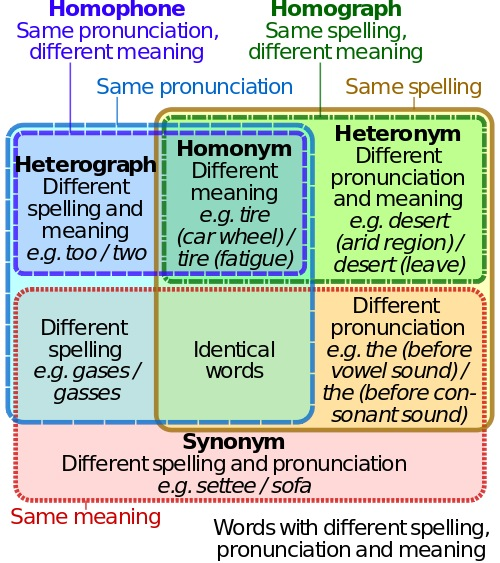
\includegraphics[width=0.5\textwidth]{500px-Homograph_homophone_venn_diagram.jpg}
\captionfonts
\caption[Word Categorization Venn Diagram]{A word categorization Venn Diagram that shows the different terms for variations in word spelling, pronunciation, and meaning. }
\label{fig:vocab:wordCategorizationDiagram}
\end{figure}

\subsection{Homographs}
\label{section:Homographs}


Homographs are orthographic words that are spelled identically. Typically, homographs are also pronounced differently, which makes them homographic heterophones(~\ref{fig:vocab:wordCategorizationDiagram}). For example, there are two homographs for the word ``does, because it has two different pronunciations: the ``multiple female deer'' does (doze), and the ``third-person singular present indicative form of `do' '' does (duhz). If the words are spelled identically AND pronounced identically, then then are homographic homophones, which are commonly known as homonyms.


\subsection{Heterographs}
\label{section:Heterographs}

Heterographs are orthographic words that are spelled differently. Typically, words are only called heterographs if they are also pronounced differently, making them heterographic homophones. Most words in the English language are heterographic heterophones; that is, spelled and pronounced uniquely. Because this is the default state of a word set, we rarely describe such words in terms of homo\slash hetero phones\slash graphs.  As such, the only time a word set is likely to be described as heterographic is if it is also a homophone. For example, the banes of every grammarian, ``there'', ``their'', and ``they're'', are heterographic homophones. Alternatively, ``to'', ``too'', and ``two'' are also heterographic homophones.  

\subsection{Homophones}
\label{section:Homophones}

Homophones are orthographic words that are pronounced identically, but typically spelled differently. If a homophone set is also homographic (that is, spelled identically as well as pronounced identically), then we refer to them as homonyms. As such, the only time the words in a set are likely to be labelled ``homophones'' is if they are also heterographic.

\subsection{Homonyms}
\label{section:Homonyms}

Homonyms are orthographic words that are pronounced and spelled identically, but defined differently. For example, depending on context, the word ``left'' can mean left (the opposite of right), or left (the past tense of leave). Homonyms can also be referred to as homographic homophones.


\section{Phonetics and Phonology}
\label{vocab:phoneticsAndPhonology}
To discover oronyms for a phrase, we must first to translate the root orthographic phrase to a representation that allows us to unambiguously measure pronunciation.   Phonology and phonetics are branches of linguistics that deal with pronunciation.

\subsection{Phonetics}
\label{vocab:phonetics}
Phonetics is a branch of \emph{descriptive} linguistics, and refers to the study of the actual, uttered sound of human speech. It deals with describing the physical phenomena of how these sounds are produced from the vocal tract, how they are transmitted once spoken, and how they are recieved by audiences. The building blocks of phonetics are \emph{phones}, which represent atomic sounds.

\subsection{Phonology (aka phonemics)}
\label{vocab:phonology}
Phonology is a branch of \emph{theoretical} linguistics, and as such, is primarily concered with the abstract grammatical characterization of sounds.  It describes the way that sounds function within a language to give meaning to words.  The basis of phonological analysis is the grouping of sounds (\emph{phones}) into distinct units within a languages.  These distinct units are called \emph{phonemes}.  

These phonemes may contain different phones, depending on the accent of the speaker.  For example, native speakers of General American English only generally recognize one `L' sound phoneme. However, there are two different ways that that phoneme manifests itself: the `l' in ``male", and the `l' in late. This difference is not noticable to a native speaker of American English, because that particular accent will parse any `L' phone as the same `L' phoneme. It would, however, be recognizable to someone whose accent categorizes those phones into two separate phonemes.

\subsection{Phonetics Vs Phonology}
\label{vocab:phoneticsVsPhonemics}

Though the terms are sometimes used interchangably, the words `phonemic' and `phonetic' (and their corresponding sound building blocks, `phone' and `phoneme')  indicate different stages of sound parsing.  \emph{Phonemes} are idealized sounds; \emph{phones} are the actual sounds that come out of a person's mouth.  Figure ~\ref{fig:knightsPhoneticPhonemic} provides a final, illustrative metaphor of the difference.
%\begin{center}
\begin{figure}[b]
\centering
        \begin{subfigure}[b]{0.4\textwidth}
                \centering
                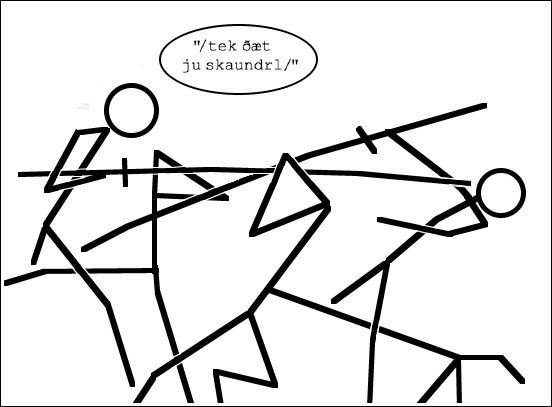
\includegraphics[width=\textwidth]{knights_phonemic.jpg}
                \captionfonts
                \caption[Phonemic Knights]{Phonology\cite{cartoonPhonemic} }
                \label{fig:cartoonPhonemic}
        \end{subfigure}
        \quad
        \begin{subfigure}[b]{0.4\textwidth}
                \centering
                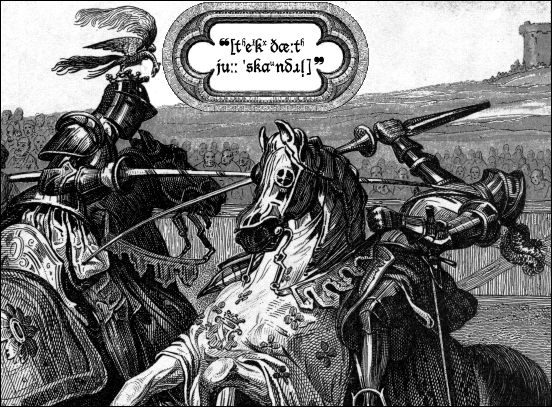
\includegraphics[width=\textwidth]{knights_phonetic.jpg}
                \captionfonts
                \caption[Phonetic Knights]{Phonetics\cite{cartoonPhonetic} }
                \label{fig:cartoonPhonetic}
        \end{subfigure}
\caption{The difference between phonetics and phonology}\label{fig:knightsPhoneticPhonemic}
\end{figure}
%\end{center}    

\FloatBarrier

\section{Phonemic/Phonetic Alphabets}
\label{section:phonemicAlphabets}
\begin{wrapfigure}{r}{0.5\textwidth}
\begin{center}
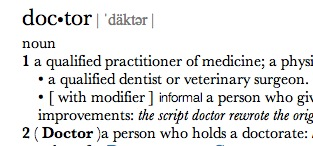
\includegraphics[width=70mm]{doctorDictIPAScreenshot.jpg}
\captionfonts
\caption[Dictionary IPA screenshot]{ The characters to the right of the large bold word ``doctor" are IPA symbols. }
\label{fig:doctorDictIPAScreenshot}
\end{center}
\end{wrapfigure}

As we stated in section~\ref{vocab:phonology}, phonemes are the atomic building blocks of words. In a phonemic alphabet, every meaningful sound has its own ``letter''.  The way that we interact with phonemes in a concrete, textual way is by using phonetic alphabets and phonetic dictionaries.  

The most common phonetic alphabet is the IPA (International Phonetic Alphabet). It contains representations of every sound in every known language globally, and allows for cross-cultural pronunciation guidelines.  As shown in figure~\ref{fig:doctorDictIPAScreenshot}, IPA representations of orthographic words are found in traditional dictionaries to aid pronunciation. 

\subsection{SAMPA}
\label{section:sampaAlphabet}

SAMPA (Speech Assessment Methods Phonetic Alphabet) is a computer-readable phonetic alphabet, based upon the symbols found in the more-standard-but-not-easily-computer-readable  IPA (International Phonetic Alphabet).  
It uses ``letters" consisting of 1-2 ASCII characters to represent each phoneme. The ASCII sequences corresponding to each of the SAMPA letters are designed so that any SAMPA sequence is deterministically parsible.

We chose to use SAMPA instead of IPA because its ASCII-compliance makes it easy to integrate into other systems.

See the table in appendix ~\ref{appendix:table:sampaTable} for a full table of each SAMPA phoneme, its description, and its sub-parts.

For some brief examples, the SAMPA spelling of the name `Jenee Hughes' is \emph{dZEni hjuz}.  
`Dr Zoe Wood'  becomes \emph{dAkt@\char18r zoui wUd}.  
`Dr John Clements' becomes \emph{dAkt@\char18r dZAn klEm@nts}. 
`Dr Franz Kurfess' becomes \emph{dAk@\char18r fr\{nz k3\char18rfEs}.



\chapter{Introduction}
\label{intro}

Human brains are built to come to single conclusions about things that have more than one interpretation.  The way that you come to this end conclusion is dependent upon your experiences, cutural immersion, and language familiarity \cite{smith_music_2003}. When attempting to write English phrases that will be read aloud and heard by people with other linguistic biases than you, it's important to make your prose as deterministically understandable as possible. The first step towards this is understanding and identifying how many ways a particular textual phrase be misheard, and why.


\section{You and me...and Leslie?}
\label{sect:youAndMeAndLeslie}

In the song \textit{``Groovin' (on a Sunday Afternoon)''}, by the Young Rascals, there's a part in the bridge that many people hear as \textit{``Life would be ecstasy, you an' me an' Leslie''}. In fact, the line is \textit{``Life would be ecstasy, you and me endlessly''}. The confusion lies with the last three syllables of the phrase. The pronunciation of each version, if spoken normally, is as follows:



%\begin{table}
\begin{center}
    \begin{tabular}{|l|c|c|}
        \hline
        \textbf{Orthographic:} & and       Les-   lie & end-       less-       ly \\ 
        \hline
        \textbf{SAMPA:}      & @nd   ``lEs     li   & ``End      l@s       li   \\
        \hline
    \end{tabular}
\label{table:groovinAlphaSAMPA}
\end{center}
%\end{table}


In the song, the singer is doing what many singers are taught to do, to make it easier to sustain the singing of words that end with difficult-to-sing consonants: the unsingable consonant is displaced onto the front of the next word. In this case, the consonant ``d'' is not singable, so he displaces it onto the next syllable, when he can: ``and ME'' becomes ``an dME'', and ``end LESS'' becomes ``en dLESS''. 

Basically, singers are *born* to ignore syllable boundries. So, our singer can effectively think of the sung phrase as:

\begin{center}
YOU an dME en dLESS lee
\end{center}

This does not cause confusion for listeners, because they are used to hearing it. This does mean, however, that lyric placement does not provide an accurate barometer to a listener of where a word actually ends.

In addition, the singer is singing fudging his vowels, like singers are taught to do, so ``and'' and ``end'' sound almost indistinguishable. So, really, what listeners are hearing is this:

\begin{center}
YOU en dME en dLESS lee
\end{center}

 Now, the listener's brain has to take this syllabic gobbledy-gook, and parse it into something useful. They've currently got this mess to deal with (represented in SAMPA syllables):

\begin{center}
{\large \textit{\textbf{ju }}}{\large \textit{En }}{\large \textit{\textbf{dmi 
}}}{\large \textit{En }}{\large \textit{\textbf{dl@s }}}{\large \textit{li}}
\end{center}

 They parse the first part just fine, because the emphases match:

\begin{center}
{\large \textbf{you }}{\large and }{\large \textbf{me }}{\large \textit{En }}{\large \textit{\textbf{dl@s 
}}}{\large \textit{li}}
\end{center}

But no one says endLESSly. People say ENDlessly. So, the listeners don't recognize it. They have to work with what they have. They already turned one ``En d'' into an ``and'', so they do it again:

\begin{center}
{\large \textbf{you }}{\large and }{\large \textbf{me }}{\large and }{\large \textit{\textbf{l@s 
}}}{\large \textit{li}}
\end{center}

Now, they're just left with LESS lee. And that fits Leslie, a proper noun that fits in context and in emphasis placement. So, the final heard lyric is:

\begin{center}
{\large \textbf{you }}{\large and }{\large \textbf{me }}{\large and }{\large \textbf{Les- 
}}{\large lie}
\end{center}

The misunderstanding can be traced back to improper emphasis placement. The songwriter probably didn't even think of that, and now he's stuck: a one-hit-wonder with a misunderstood song. We bet that in interview after interview, someone asks him who Leslie is. It's probably very frustrating --- especially since he could have just moved the word an eight note later, and it would have been understood perfectly.

That's the sort of situation this program is going to help avoid.



\section{ Why it breaks down }
\label{sect:whyItBreaksDown}

There are two points at which the author's intendeded phrasing can be muddled : First, when the author's orthographic text becomes an orator's spoken (phonetic) interpretation, and second, when the orator's phonetic interpretation is translated phonetically by an audience into a perceived orthographic phrase. Both of these interpretations must be made succesfully in order for the author's intended meaning to be conveyed.


The phrase ``iced ink" undisputedly succeeds in the first translation, but fails on the second.  Iced ink can only be pronouced one way, but it can be heard multiple ways--the most notable of which is ``I stink", not ``iced ink".

The phrase ``a nice cold hour" can fail on both parts.  First, the orator could have accidentally-capitalized the word Nice in their head, and made it sound like Nice, the city in France.  An audience would likely hear this as ``niece", and would be confused, at best.  Even if the orator pronouces the phrase as the author intended, the audience could hear multiple orthographic phrases in the same phonetic sequence: ``a nice cold hour", ``an ice cold hour", or even ``a nigh scold our".

A third, more rare and nefarious type of audience misunderstanding can be caused by parse-tree misdirection, where an audience member is absolutely sure they're hearing one phrase, only to get lost halfway through the lyric because they though they were interpreting a phonetic sequence in a way that resulted in an orthographic dead end. This happens due to the relative frequency of the possible lyrics heard.

 For example, when asked to sing along with the Adele song, Rolling in the Deep, people who were starting to sing enthusiastically dropped out around the line ``reaching a fever pitch"\cite{frontPorchBandAdeleCover}.  Let us consider the phrase ``fever pitch".  This phrase has no exact oronyms, but it does have a potential dead end-- a listener could hear the first syllable of the phrase as the word ``fee", which has a frequency of 7265.  That's more than double the frequency of the word ``fever", which is 3095.  

Looking at the oronym parse tree for the phrase ``fever pitch" in figure ~\ref{fig:feverPitchOronymTree}, we can see that the branch for ``fever" ends in a much smaller radius than the branch on the left for the word ``fee".  As you can see by the relative size of the end spheres of the branches, the word ``fee" even outweighs the last word in the other branch as well (which is ``pitch" with a frequency of 5104). Since the human brain is pre-disposed to parse more-familiar words, having that heavily-weighted dead-end branch is likely the cause of the casual listener not being able to memorize the lyrics.
\begin{wrapfigure}{r}{0.5\textwidth}[h]
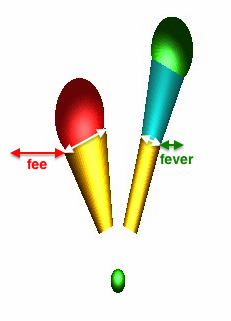
\includegraphics[width=.5\textwidth]{feverPitchTreeAnnotated.jpg}
\captionfonts
\caption[Annotated Oronym Parse tree  generated for the phrase ``fever pitch"]{ Annotated Oronym Parse tree generated for the phrase ``fever pitch" }
\label{fig:feverPitchOronymTree}
\end{wrapfigure}





%%%%\include{relatedWork}
%%%%%\chapter{Background}
\label{background}

\textcolor{Red}{I think I decimated this section when I wrote the Preliminary Vocab section.  Is there something else that should go here?}


\chapter{Implementation}
\label{implementation}
We present a computer program which takes in textual phrases in English, determines all oronyms for that phrase and then visualizes them with associated information to indicate the likelihood of interpretation.
To accomplish this, the program has three major functional parts: a custom phonetic dictionary, a command-line oronym generator, and a OpenGL oronym-parse-tree visualization generator.

\section{Customized Phonetic Dictionary} 
\label{section:Implementation:customizedPhoneticDictionary}

In order to discover oronyms for each phrase, we first needed to determine how each phrase is pronounced.  Pronunciation can vary depending on the speakers accent, so it was important for us to (1) chose an accent that we could easily replicate and (2) find a dictionary that supported that accent.  

We decided to utilize a General American accent, due to its ubiquity in media and news sources. The General American accent, also known as the ``Standard American English" dialect, is not spoken by the majority of people in America, but is used as an ``average accent".  It most closely resembles the Midwestern accent using in the area in Figure ~\ref{fig:generalAmericanMap} and more commonly recognized as ``the newscaster accent". Newscasters learn this accent for national TV, because it is the ``least-accented" of the American accents.  

\begin{center}
\begin{figure}
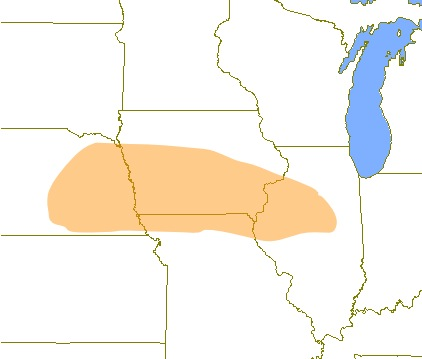
\includegraphics[width=60mm]{General_American.jpg}
\captionfonts
\caption[Geographic Origin of General American]{This is the geographic area whose accent most closely resembles the General American Accent \cite{generalAmericanAccentMap} }
\label{fig:generalAmericanMap}
\end{figure}
\end{center}

\subsection{Dictionary Options}
\label{subsection:dictionaryOptions}

We considered using three different phonetic dictionaries: the CMU dictionary, LC-STAR dictionary and UNISYN dictionary\cite{lcStarWebsite} \cite{cmuDictWebsite}  \cite{unisynLexiconWebsite}.  We started out by looking at the LC-STAR dictionary, but quickly decided that it wasn’t going to be as useful to us, because the LC-Star project is relatively focused on Speech-to-Speech or Text-to-Speech tech. In addition, the dictionary is not well-maintained.  

The CMU dictionary showed promise, but had a few shortcomings.  It had a very simple way of encoding words:  first the word, then the identifier number in parens (if needed), then a space, then a one-to-two char code for each sound in the word, with the numbers 0, 1, 2 appended to indicate emphasis (if needed), separated by spaces.  An example of a CMU dictionary entry can be seen in Figure ~\ref{fig:CMUdictAbbreviate}.

\begin{figure}
\begin{center}
\begin{verbatim}
ABBREVIATE  AH0 B R IY1 V IY0 EY2 T
\end{verbatim}
\captionfonts
\caption[CMU dictionary entry example]{Here is the CMU dictionary entry for the word ``abbreviate" }
\label{fig:CMUdictAbbreviate}
\end{center}
\end{figure}

The problem that arose with this format, was that there was no explicit definition of where to hyphenate the word when splitting it up.  This causes problems for words in song lyrics, where each note has its own syllable underneath it, and each syllable might have many different sounds. 
The benefits of the CMU dictionary over some other dictionaries were that (1) it was actively maintained, (2) it included proper nouns, which are often found in lyrics, but not in dictionaries, and (3) it was ridiculously easy to read.

The downsides were that (1) it included no part of speech data or hyphenation data, and (2) it used non-standard symbols for its phonetic alphabet.  
With the downsides and benefits in mind, the CMU dictionary could not be used in isolation, especially if we someday want to attempt generation of original lyrics (which part of speech data would be vital for).  

The UNISYN dictionary is used primarily to phonetically translate words into multiple accents.  It has its own formated dictionary, with a bunch of wildcards in it.  They also provide some semi-functioning perl scripts that allow you to specify a dialect you’d like to use (For example, a Californian would say “cooking” differently than someone from the Deep South, and both would say it differently than someone from London.  However, they are all speaking English.  The UNISYN dictionary facilitates this translation).  

It had all the information we needed, and then some.  However, it was case-insensitve, meaning that it didn't make it easy to differenciate pronunciations for some words. For example, the word ``nice" is pronounced differently from the city ``Nice", but they were both stored as ``nice" in the orthography of UNISYN.  The CMU dictionary did keep track of capitalization.  The obvious conclusion, then, was to grab the capitalizations from the CMU dictionary and put them in the UNISYN dictionary, aligning them by pronunciation and part of speech. 

However, we ran into a setback, mentioned in the very first article we found references to both dictionaries in:  the dictionaries were inconsistent\cite{polyakova_fusion_2007}.  They didn’t always put stresses in the same place, nor did they always have the same pronunciation.  Because of this, it was difficult to match words, especially words that were homographic heteronyms (same writing, different sounds, like ``Do you know what a buck \emph{does} to \emph{does}?").  Because of this, we decided to use the UNISYN dictionary exclusively.

\subsection{Custom dictionary fields}
\label{subsection:customDictionaryFields}

Here is the format for the fields in an entry in our custom phonetic dictionary, after we were done with fixing the UNISYN output:
\begin{center}
\textcolor{Aquamarine}{$<$\textbf{ortho}$>$} :
\textcolor{BurntOrange}{$<$\textbf{uniqueID}$>$} :
\textcolor{RoyalBlue}{$<$\textbf{partOfSpeech}$>$} :
\textcolor{Red}{$<$\textbf{SAMPAspelling}$>$} :
\textcolor{Rhodamine}{$<$\textbf{SAMPAnoEmph}$>$} :
\textcolor{Periwinkle}{$<$\textbf{extendedOrtho}$>$} :
\textcolor{Blue}{$<$\textbf{freq}$>$}
\end{center}

\begin{figure}
Example:
\begin{center}
{\tt 
\textcolor{Aquamarine}{transfer} :
\textcolor{BurntOrange}{2} :
\textcolor{RoyalBlue}{VB/VBP} :
\textcolor{Red}{tr\{ns"f3`r} :
\textcolor{Rhodamine}{tr\{nsf3`r} :
\textcolor{Periwinkle}{\{trans==fer\}} :
\textcolor{Blue}{7184}
}
\captionfonts
\caption[Custom dictionary entry example]{Here is an example an entry in our custom phonetic dictionary, using the word ``transfer" }
\label{fig:customDictionaryEntryExample}
\end{center}
\end{figure}

\textcolor{Aquamarine}{$<$\textbf{ortho}$>$} is the regular spelling of the word

\textcolor{BurntOrange}{$<$\textbf{uniqueID}$>$} is a number (and optional string) used to differentiate homographs.

\textcolor{RoyalBlue}{$<$\textbf{partOfSpeech}$>$} is used to identify the specific part of speech

\textcolor{Red}{$<$\textbf{SAMPAspelling}$>$} is the breakdown of the word, phonetically. It uses the SAMPA alphabet, and separators to show where breaks in the word are, and how they’re emphasized. If a separator is ' \$ ', the following phones (until the next separator) are not emphasized.  If it's ' \% ', then they are the secondary emphasis.  If it's ' `` ', then they are the primary emphasis.

\textcolor{Rhodamine}{$<$\textbf{SAMPAnoEmph}$>$} is the same as \emph{<SAMPASpelling>}, but with all emphasis characters stripped out.  We chose to add this field so that we could more-easily look up phonetic sequence matches. 

\textcolor{Periwinkle}{$<$\textbf{extendedOrtho}$>$} allows for stemming analysis of words, for possible use in future work.

\textcolor{Blue}{$<$\textbf{freq}$>$} is the frequency at which the word occurs in language, according to UNISYN. The frequency count is ``taken from a composite of a number of on-line sources of word-frequency. It includes frequencies from the British National Corpus and Maptask, and frequencies derived from Time articles and on-line texts such as Gutenberg. They were weighted to give more importance to sources of spoken speech, and also to increase the numeric frequency of smaller corpuses"\cite{fitt_documentation_2000}.


An example of a entry in our custom phonetic dictionary can be seen in \textbf{Figure ~\ref{fig:customDictionaryEntryExample} }.
\subsection{Transferring the dictionary to a sqlite database}
\label{subsection:transferringTheDictionaryToASqliteDatabase}

Because there are several hundred thousand entries in our phonetic dictionary, it was necessary to have a database, rather than store them all in-program in a multi-dimensional array.  We decided to use a SQLite database for this purpose.  

To turn the colon-delimited dictionary file into a SQLite database, we decided to use a program called the “SQLite Database Browser”, an open source, public domain, freeware visual tool to create, design, and edit SQLite3.x database files.  We specifically used version 2.0b1 of the program, which was built with version 3.6.18 of the SQLite engine\cite{sqliteDatabaseBrowser}.

\section{Oronym Generation}
\label{oronymGeneration}

\subsection{Step 1: Find all phonemic variations of an orthographic phrase}
\label{subsection:stepOneFindAllSAMPAphrase}

First, our program takes an orthographic phrase to find oronyms for.

\begin{figure}[h]
\begin{center}
\begin{tabular}{|c|}
\hline
`a nice cold hour' \\
\hline
\end{tabular}
\label{fig:oronymGeneration:orthoPhraseInput}
\end{center}
\end{figure}

We then tokenize this phrase into its component words, using whitespaces as a delimiter. 
\begin{figure}[h]
\begin{center}
\begin{tabular}{|c|}
\hline
`a', `nice', `cold', `hour' \\
\hline
\end{tabular}
\label{fig:oronymGeneration:tokenizedInputOrthoPhraseWords}
\end{center}
\end{figure}


For each word in the phrase, we query our phonetic dictionary for all possible SAMPA pronunciations.

\begin{figure}[h]
\begin{center}
\begin{tabular}{|c|}

\hline
`a' \rightarrow  \tt{e}, \tt{@}, \tt{A} \\

`nice' \rightarrow   \tt{naIs}, \tt{nis} \\

`cold' \rightarrow \tt{kould} \\

`hour' \rightarrow \tt{aU\char18 r} \\
\hline
\end{tabular}
\captionfonts
\caption[queryDBwithOrthoWordForSampa example]{ In this and all subsequent diagrams, a `string in quotes' indicates an orthographic word or phrase, and a \texttt{monospaced string} indicates that it is a SAMPA word or phrase.  }
\label{fig:oronymGeneration:queryDBwithOrthoWordForSampa}
\end{center}
\end{figure}

Now that we have the pronunciation of each of the words in the form of SAMPA strings, we can list all the possible phonetic permutations of the original phrase.

\begin{figure}[h]
\begin{center}
\begin{tabular}{|c|}

\hline
e naIs kould aU\char18 r \\

@ naIs kould aU\char18 r \\

A naIs kould aU\char18 r  \\

e nis kould aU\char18 r \\

@ nis kould aU\char18 r \\

A nis kould aU\char18 r \\
\hline
\end{tabular}
\captionfonts
\caption{}
\label{fig:oronymGeneration:orthoWordPhoneticPermutations}
\end{center}
\end{figure}


The pseudocode for this process can be reviewed in figure ~\ref{fig:psuedoCode:findAllPhoneSeqsForOrthoPhrase}.

\setlength\LTleft{-2in}
\begin{figure}
\begin{verbatim}
findAllPhoneSeqsForOrthoPhrase( orthoPhrase ) {
  allFullPhrasePhoneSeqs = empty list of list of phones
  orthoWords = split orthoPhrase on spaces
  
  origNumFullPhrases = 0
  for( orthoWord in orthoWords with index i ) {
    nextWordSampaPhoneSeqs = possible phone seqs following orthoWord
    
    if ( orthoWord is the first word in orthoPhrase ) {
      for( phoneSubSeq in nextWordSampaPhoneSeqs ) {
        append phoneSubSeq to allFullPhrasePhoneSeqs[i]
      }
    } else {
      origNumFullPhrases = allFullPhrasePhoneSeqs.size()
      if there’s more than one vector <phone> in nextWordSampaPhoneSeqs
        then we need to create duplicates of all existing allFullPhrasePhoneSeqs
    }
    
    for( m = 0 to allPhrasePhoneSeqs.size() ) {
      phraseToAppendIndex = m / origNumFullPhrases
      phoneSeqToAppend = nextWordSampaPhoneSeqs[phraseToAppendIndex]
      append phoneSeqToAppend to allFullPhrasePhoneSeqs[m]
    }
  }

  return allFullPhrasePhoneSeqs
}
\end{verbatim}
\captionfonts
\caption[Pseudocode for findAllPhoneSeqsForOrthoPhrase]{ Algorithm to get all phonetic sequences for an orthographic phrase. }
\label{fig:psuedoCode:findAllPhoneSeqsForOrthoPhrase}
\end{figure}
%\setlength\LTleft{2in}



\subsection{Step 2: Finding all Orthographic phrases for a Phonemic Sequence}
\label{subsection:stepTwoFindOrthoforSAMPA}

Then, for each phonemic phrase, we want to figure out all valid orthogrpahic interpretations.  For this, we have to go back to our phonetic dictionary.

The ideal way to think about searching for words in a phonetic sequence is by picturing the phoenetic sequence in a tree form.  For example, if I had a phonetic tree with the entire dictionary in it, each phonetic tree node would have at least 45 child nodes: one for each phone.  A node might also have ``word" nodes, if the phones along the path to that node construct a valid orthographic word:

When there are multiple orthographic interpretations at a single phonetic node, the most likely interpretation can be determined by checking the frequency of use for each word.  For example, the sequence ``n aI s" is much more likely to be ``nice" than ``gneiss".  Figure ~\ref{fig:wordTree} shows a visual representation of traversing an entire dictionary's phonetic tree for nodes along the paths for the SAMPA sequences `aIs' and `nice'.

\begin{figure}[h]
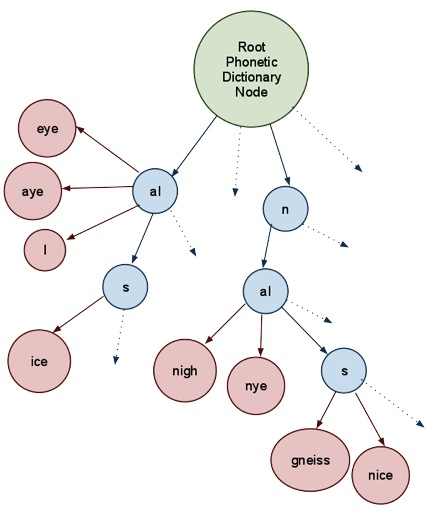
\includegraphics[width=90mm]{wordTree.jpg}
\captionfonts
\caption{}
\label{fig:wordTree}
\end{figure}

We can use this dictionary tree method to discover valid orthographic interpretations for each phonetic sequence.  Using the dictionary tree method above, we can orthographically interpret each phonetic transcription of our root orthographic phrase, as shown in figure ~\ref{fig:aNiceColdHourPhoneToOrthoGraph}:



\begin{figure}[h]
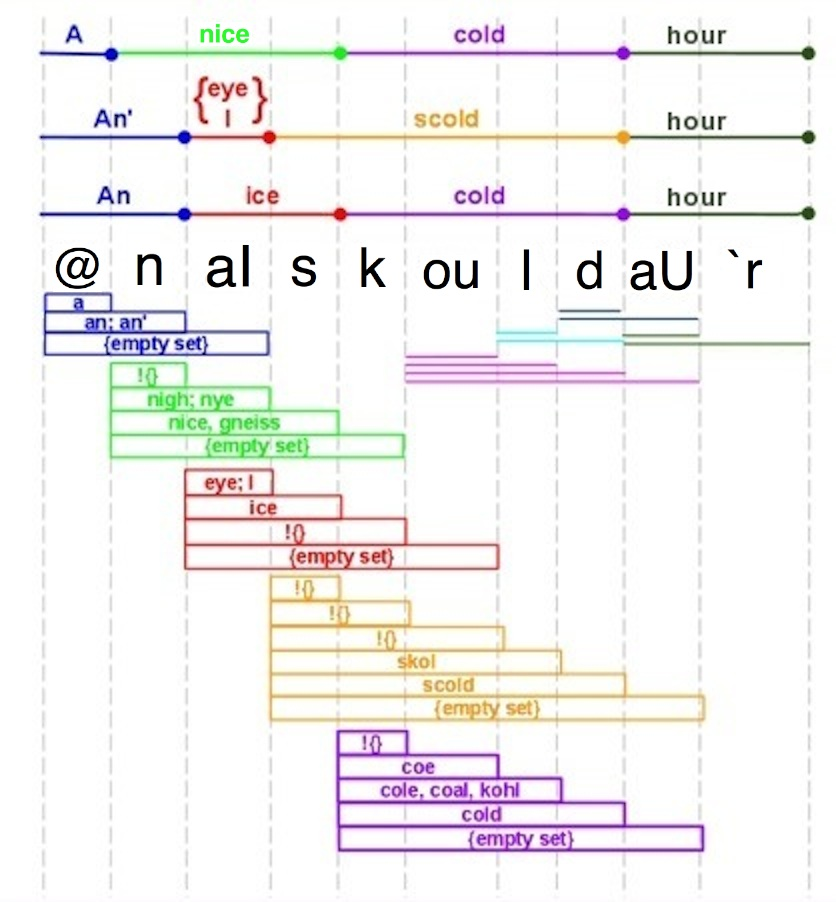
\includegraphics{aNiceColdHourPhoneToOrthoBreakdown.jpg}
\captionfonts
\caption{}
\label{fig:aNiceColdHourPhoneToOrthoGraph}
\end{figure}

Once we have grabbed all the orthographic interpretations for each phonetic sequence, we combine them all into a orthographic oronym phrase list. This process may leave us with some redundant oronyms, so we de-duplicate that list.

This process gives us a list of all unique and valid oronyms for the original root phrase.

In the case of ``a nice cold hour", this returns 290 oronyms, as seen in the first column of figure ~\ref{table:aNiceColdHourOronymWithFreqsTable}.



The pseudocode for this process can be reviewed in figure ~\ref{fig:psuedoCode:discoverOronymsForPhrase}
\setlength\LTleft{-2in}
\begin{figure}
\begin{verbatim}
discoverOronymsForPhrase( origOrthoPhrase, includeDeadends ) {
   orthoMisheardAsPhrases = empty list
   allPhoneSeqsOfOrigPhrase = origOrthoPhrase.findAllPhoneSeqs()
   
   for( curPhoneSeqWithEmph in allPhoneSeqsOfOrigPhrase ) {
      // Remove emphasis marking for easier lookups
      curPhoneSeq = curPhoneSeqWithEmph.stripEmphasis()

      altOrthoPhrases = findOrthoStrsForPhoneSeq( curPhoneSeq )
      
      for( altOrthoPhrase in altOrthoPhrases ) {
         // Ensure it contains valid ortho text in all cases, and if
         // includeDeadends=false, contains no deadEndDelims so we only add
         // fully valid strings
         if ( ( includeDeadends == true &&
                altOrthoPhrase != deadEndDelim1 &&
                altOrthoPhrase != deadEndDelim2 ) ||
              ( altOrthoPhrase.contains( deadEndDelim1 ) == false &&
                altOrthoPhrase.contains( deadEndDelim2 ) == false ) ) {
            append altOrthoPhrase to orthoMisheardAsPhrases
         }
      }
   }
   
   orthoMisheardAsPhrases.removeDuplicates()

   return orthoMisheardAsPhrases
}
\end{verbatim}
\captionfonts
\caption[Pseudocode for discoverOronymsForPhrase]{ Algorithm to get all oronyms for an orthographic phrase. }
\label{fig:psuedoCode:discoverOronymsForPhrase}
\end{figure}
\setlength\LTleft{2in}




\subsection{Word Frequency Evaluation}
\label{subsection:wordFrequencyEvaluation}

Next, we want to evaluate all our oronyms based on how common each oronym's component words are.  For example, ``a nice cold hour" is much more likely to be heard ``a gneiss cold hour", even though both are phonetically identical.

To do this, we tokenize each oronym phrase into its component words, once again using non-newline whitespaces as a delimiter. 

Then, we query our phonetic dictionary with each word for the word's frequency value.  We store each word's value separately. When we have retrieved the frequencies for all the words in a phrase, we then add all the frequencies up to give a combined-frequency of the entire phrase.

You can see these frequency counts for the phrase ``a nice cold hour" in figure ~\ref{table:aNiceColdHourOronymWithFreqsTable}.




\section{Visual Representation}
\label{section:implementation:visualRepresentation}

We go about building the visual representation of the oronym parse tree in much the same way that we build the textual list of oronyms, with one important difference: our oronym parse trees may contain oronym fragments.   To deal with these we've got to keep track of all our abandoned sub-phrases.

Our algorithm for doing this is recursive, called from a parent function that draws the tree's `seed' sphere. This parent function is documented in figure ~\ref{fig:psuedoCode:buildAndDrawFullTree}


We start in the parent function by getting all the oronyms of our orthographic phrase, using the process in sections  ~\ref{subsection:stepOneFindAllSAMPAphrase} ~\ref{subsection:stepTwoFindOrthoforSAMPA}.  However, instead of ignoring any incomplete orthographic interpretation of a phonetic sequence, as we do in section~\ref{subsection:stepTwoFindOrthoforSAMPA}, we add them to the list of oronyms, keeping track of them by appending `xxx' or `fff' to the end of the incomplete  oronym string.  Then, we tokenize our phrases by whitespace, and look up the frequency of each word, keeping track of only the maximum and minumum values.  We will later scale our branches' radiuses using these values.

Once we have all the partial and complete oronyms and the max and min word frequency values for them, we pass them into our recursive function, along with the radius of the seed sphere.  That radius will be the beginning radius of each first-level branch.  

Inside our recursive function, we pull the first word out of every orthographic phrases we were passed, and create a set of unique first words.  

We then go through this set of unique first words iteratively.

For each word, we look up frequency in the phonetic dictionary.  Then, we use the max and min frequencies that we found in our parent function, plus constants for max and min radius size, to scale that frequency into a usable radius size. 

Then, we check the contents of the word. 

If the word is ``xxx" or ``fff", then it's not a word at all--just an indication of the dead end of a partial oronym.  In this case, we draw a red sphere with the radius of the branch's ancestor, using the parameter past into our recursive function for `lastRadius'.  

If the word is ``\_\_\_SUCCESS!\_\_\_", that is also not a real word. It indicates that a full oronym has been successfully found, and is terminating at that point. This time, we draw a green sphere using the `lastRadius' parameter for size.

If the word is neither of these, then it must be a real word.  We then draw a cylinder ``branch" representing that word. The cylinder's bottom radius is equal to \emph{lastRadius}, and the top radius is equal to the scaled radius that we got from the word's frequency.  

After we draw the cylinder, we then go through the full list of phrases, and compile a list of all phrases that start with the word we just drew the cylinder for.  Then, we remove the first word from each of those phrases, deduplicating the resulting list of ``tail" phrases.

Then, we change our material color (so that different levels of branches will be different colors), and make a recursive call to our current function, passing as parameters the scaled radius and the list of tail phrase.

After this recursive call, we change our color material back to whatever it was before the call, and then continue on to the next unique first word in our set.


Once we have looped through all our unique first words, we know we're done drawing that set of branches, and we return.  

This gives us the oronym parse tree seen in figure ~\ref{fig:treeEmptyTillIsSad}.  As shown in figure ~\ref{fig:treeEmptyTillIsSadAnnotated} (the annotated version of figure ~\ref{fig:treeEmptyTillIsSad}) each branch on the tree represents a single orthographic word.


\begin{figure}
\begin{verbatim}
buildAndDrawFullTree( orthoPhrase ) {
   fullPhrases = orthoPhrase.discoverOronyms()
   (maxWordFreq, minWordFreq) = fullPhrases.getMaxAndMin()
   
   // Draw the tree's seed.
   glPushMatrix()
   {
      glTranslated(0.0, -1.0 * DEFAULT_BRANCH_LEN, 0.0)
      materials(GreenShiny)
      drawSphere(DEFAULT_RADIUS)
      materials(allMaterials.at( mat % allMaterials.size() ) )
      
      drawBranchesAtFork ( fullPhrases, DEFAULT_RADIUS )
   }
   glPopMatrix()
}
\end{verbatim}
\captionfonts
\caption[Code for buildAndDrawFullTree]{ Given an orthographic phrase, this function prepares to draw the tree }
\label{fig:psuedoCode:buildAndDrawFullTree}
\end{figure}


\begin{figure}
\begin{adjustwidth}{-1in}{}
\begin{verbatim}
drawBranchesAtFork( fullPhrases, lastRadius) {
   if( fullPhrases.size() == 0 ) {
      return
   }
   
   // Use a set to ensure no duplicates.
   firstWords = empty set
   
   for( phrase in fullPhrases ) {
      if( phrase.size() > 0 ) {
         firstWords.insert( phrase.firstWord() )
      }
   }
   
   // Calculate positioning variables for the spread of branches for firstWords.
   for ( curFirstWord in firstWords ) {
      firstWordFreq = curFirstWord.frequency()
      newAdditiveRadius = firstWordFreq.scaleToRadius()

      glPushMatrix()
      {
         // Translate and rotate into place
         if( curFirstWord == deadEndDelim1 || curFirstWord == deadEndDelim2 ) {
            // Draw a red sphere at the end of the last branch
         } else if ( curFirstWord == successDelim ) {
            // Draw a green sphere at the end of the last branch
         } else {
            // Draw a branch
            drawBranch( radiansToDegrees(tiltAngle), curXOffset, curYOffset,
                        newAdditiveRadius, lastRadius )
            
            // Find all phrases in fullPhrases that start with that firstWord
            tailsVect = fullPhrases.findAllWithPrefix(curFirstWord)
            
            // Change the colors for each branch level

            // Pass those phrases to drawBranchesAtFork
            drawBranchesAtFork( tailsVect, newAdditiveRadius, curXOffset, curYOffset )
            
            // Change the colors back to ensure consistency for each branch level
         }
      }
      glPopMatrix()
   }
}
\end{verbatim}
\end{adjustwidth}
\captionfonts
\caption[Code for drawBranchesAtFork]{ This is the function that facilitates the in-time drawing of the tree as we parse though our oronyms possibilities }
\label{fig:psuedoCode:drawBranchesAtFork}
\end{figure}

At the end of this process, we have generated a tree like the one in figure ~\ref{fig:treeEmptyTillIsSad}.  Each branch represents a word, as can be seen in figure ~\ref{fig:treeEmptyTillIsSadAnnotated}.


\begin{figure}
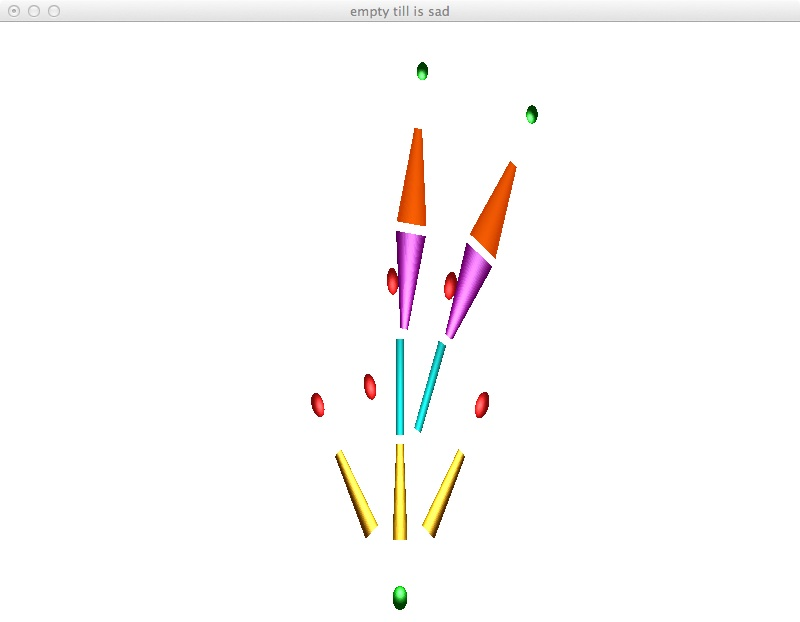
\includegraphics[width=150mm]{emptyTillIsSad.jpg}
\captionfonts
\caption[Oronym Parse Tree]{ This is the parse tree for the phrase ``empty till is sad" }
\label{fig:treeEmptyTillIsSad}
\end{figure}

\begin{figure}
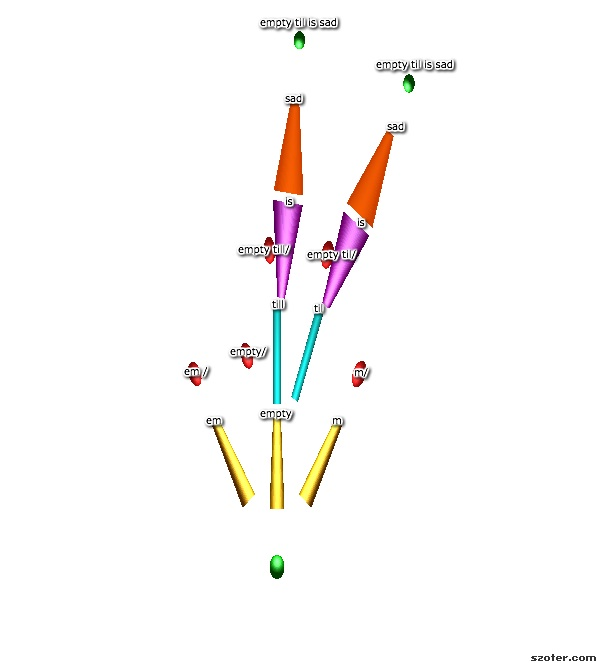
\includegraphics[width=150mm]{emptyTillIsSadAnnotated.jpg}
\captionfonts
\caption[Annotated Oronym Parse Tree]{ This is the annotated parse tree for the phrase ``empty till is sad" }
\label{fig:treeEmptyTillIsSadAnnotated}
\end{figure}






\chapter{User Study}
\label{userStudy}

\section{Structure} We created a multi-wave user study to examine the effectiveness of different parts of our program. 

In the first phase, we had \uniqueUsersPhaseOneUserStudy people record over \numResponsesPhaseOneUserStudy different phrases, to see how they pronouced them.  This phase served two purposes: one, to gather recordings for the second phase, and two, to see if our phonemic transcriptions were valid.  

In the second phase, we took \recordingsPhaseTwoUserStudy recordings of oronyms from phase one, and gathered \numTranscriptionsPerRecordingPhaseTwoUserStudy transcriptions for each recording, resulting in a total of \numResponsesPhaseTwoUserStudy transcriptions. These transcriptions were provided by \uniqueUsersPhaseTwoUserStudy unique users ( \uniqueUsersPhaseTwoUserStudyUSA from the United States).  We then compared the transcriptions of the recorded oronym phrases to the calculated oronyms for the original root phrase.

\section{User Sampling Population}
We drew our test subjects from a pool of Amazon Mechanical Turk workers (hired for \$ 0.02 to \$ 0.10 per task) and, for part of phase 1, volunteers from Reddit.com \cite{redditAssistance} \cite{redditRecordThis}. 

Amazon Mechanical Turk is an online crowdsourcing service where requesters can hire workers to complete Human Intelligence Tasks, or HITs.  The efficacy of using Mechanical Turk for user studies has been widely studied in academia, and specifically proven in the linguistic community \cite{sprouse_validation_2011}.


\section{Methodology}

\subsection{First Phase: Recitation}
\label{subsection:firstWaveUserStudy}
In this wave of the user study, we used a combination of \uniqueUsersPhaseOneUserStudy Mechanical Turk workers (hired for \$ 0.10 per task) to record \numResponsesPhaseOneUserStudy different phrases.  These phrases were oronyms of one of two phrases: phrase A, ``a nice cold hour" or phrase B, `` fourth rye to".  To keep track of the phrases, we assigned each phrase an phraseID, built off of the phrase letter, phrase length, and phrase text.    We gave Mechanical Turk workers three minutes to record each phrase and email it to us with the phrase identifier in the subject of the email. The number of recordings per phrase, along with their identifiers, can be seen in table ~\ref{table:phrasesRecorded}.


\begin{center}

%\begin{table}

\begin{longtable}{|c|c|c|}
\caption[Phrases Recorded]{Here are the phrases we recorded, how many times they were recorded, and the identifiers we used for each phrase}
\label{table:phrasesRecorded} 

\hline 
orthoPhrase & numRecordings & phraseID \\
\endfirsthead

\multicolumn{3}{c}%
{{\bfseries \tablename\ \thetable{} -- continued from previous page}} \\
\hline
orthoPhrase & numRecordings & phraseID \\
\endhead


\hline \multicolumn{3}{|r|}{{Continued on next page}} \\ \hline
\endfoot

\hline \hline
\endlastfoot

\hline
a nice cold our   & 3 & A.17.51    a nice cold our  \\
\hline
an ice cold our   & 2 & A.17.135    an ice cold our  \\
\hline 
a nye scold our   & 2 & A.17.69    a nye scold our  \\
\hline 
ah nye scold our   & 2 & A.18.109    ah nye scold our  \\
\hline 
an eye scold our   & 2 & A.18.125    an eye scold our  \\
\hline 
on aye scold our   & 2 & A.18.267    on aye scold our  \\
\hline 
a nigh scold our   & 2 & A.18.65    a nigh scold our  \\
\hline 
a nye skol dower   & 2 & A.18.71    a nye skol dower  \\
\hline 
an aye skol dower   & 2 & A.19.119    an aye skol dower  \\
\hline 
an eye skol dower   & 2 & A.19.127    an eye skol dower  \\
\hline 
an ice coal dower   & 2 & A.19.133    an ice coal dower  \\
\hline 
eh nice coal dower   & 2 & A.20.159    eh nice coal dower  \\
\hline 
ah nice coal dower   & 2 & A.20.89    ah nice coal dower  \\
\hline 
fourth wry to   & 2 & B.15.19    fourth wry to  \\
\hline 
fourth wry too   & 2 & B.16.20    fourth wry too  \\
\hline 
forth right ooh   & 2 & B.17.1    forth right ooh  \\
\hline 
fourth rite ooh   & 2 & B.17.13    fourth rite ooh  \\
\hline 
forth wright ooh   & 2 & B.18.6    forth wright ooh  \\
\hline 
on i scold our   & 1 & A.16.279    on i scold our  \\
\hline 
an i scold hour   & 1 & A.17.128    an i scold hour  \\
\hline 
an i skol dower   & 1 & A.17.131    an i skol dower  \\
\hline 
an ice-cold our   & 1 & A.17.141    an ice-cold our  \\
\hline 
on i scold hour   & 1 & A.17.278    on i scold hour  \\
\hline 
on i skol dower   & 1 & A.17.281    on i skol dower  \\
\hline 
an aye scold our   & 1 & A.18.117    an aye scold our  \\
\hline 
an ice cold hour   & 1 & A.18.134    an ice cold hour  \\
\hline 
an ice-cold hour   & 1 & A.18.140    an ice-cold hour  \\
\hline 
eh nye scold our   & 1 & A.18.179    eh nye scold our  \\
\hline 
on eye scold our   & 1 & A.18.275    on eye scold our  \\
\hline 
on ice cold hour   & 1 & A.18.284    on ice cold hour  \\
\hline 
on ice-cold hour   & 1 & A.18.290    on ice-cold hour  \\
\hline 
a nye scold hour   & 1 & A.18.68    a nye scold hour  \\
\hline 
ah nice cold our   & 1 & A.18.91    ah nice cold our  \\
\hline 
ah nigh scold our   & 1 & A.19.105    ah nigh scold our  \\
\hline 
ah nye scold hour   & 1 & A.19.108    ah nye scold hour  \\
\hline 
ah nye skol dower   & 1 & A.19.111    ah nye skol dower  \\
\hline 
an aye scold hour   & 1 & A.19.116    an aye scold hour  \\
\hline 
an ice kohl dower   & 1 & A.19.139    an ice kohl dower  \\
\hline 
eh nice cold hour   & 1 & A.19.160    eh nice cold hour  \\
\hline 
eh nigh scold our   & 1 & A.19.175    eh nigh scold our  \\
\hline 
eh nye skol dower   & 1 & A.19.181    eh nye skol dower  \\
\hline 
on aye skol dower   & 1 & A.19.269    on aye skol dower  \\
\hline 
on eye scold hour   & 1 & A.19.274    on eye scold hour  \\
\hline 
on ice coal dower   & 1 & A.19.283    on ice coal dower  \\
\hline 
on ice kohl dower   & 1 & A.19.289    on ice kohl dower  \\
\hline 
a nice coal dower   & 1 & A.19.49    a nice coal dower  \\
\hline 
a nigh scold hour   & 1 & A.19.64    a nigh scold hour  \\
\hline 
ah nice cold hour   & 1 & A.19.90    ah nice cold hour  \\
\hline 
eh nice cole dower   & 1 & A.20.163    eh nice cole dower  \\
\hline 
eh nigh scold hour   & 1 & A.20.174    eh nigh scold hour  \\
\hline 
eh nigh skol dower   & 1 & A.20.177    eh nigh skol dower  \\
\hline 
ah nice cole dower   & 1 & A.20.93    ah nice cole dower  \\
\hline 
ah nice kohl dower   & 1 & A.20.95    ah nice kohl dower  \\
\hline 
forth wry two   & 1 & B.15.10    forth wry two  \\
\hline 
forth rye two   & 1 & B.15.5    forth rye two  \\
\hline 
forth write ooh   & 1 & B.17.7    forth write ooh  \\
\hline 
fourth right ooh   & 1 & B.18.12    fourth right ooh  \\
\hline 
fourth wright ooh   & 1 & B.19.17    fourth wright ooh  \\
\hline

\end{longtable}

%\end{table}
\end{center}

We then transcribed the phonetics of each of the recording in SAMPA by ear.  In a stunning example of a use case for our project, we discovered that we had unintentionally included some phrases for recordings were not deterministically phonetically parsible, meaning that our oronyms had multiple pronunciations, not all of which mapped back to the original phrase.  For example, the orthographic word ``a" can be interpreted as the phoneme `A', and that `A' phoneme can be combined with the subsequent `n' phoneme from the word ``nice" to create the SAMPA sequence `An'.  That being said, this fit with our model, and we found no unexpected anomalies when comparing our transcriptions to the expected SAMPA spellings of each phrase.




\subsection{Recording Sample Pool}
\label{subsection:recordingSamplePool}
We had originally intended to use all the phase one recordings in phase two, but eventually had to discard all but \recordingsPhaseTwoUserStudy of the recordings for various reasons, the most common being that the recording was too loud and we wanted to spare our user's ears, or the person recording left excessive amounts of space between words that overly-segmented the phrase.  The recordings for the ``fourth rye to" oronyms were all unusable for phase two, because our users tended to insert exclamation points any time they said ``ooh" or ``too", overloading their microphones or over-segmenting the phrase.

All \recordingsPhaseTwoUserStudy recordings we used were oronyms for the phrase ``a nice cold hour", and were recorded by one man with remarkably smooth diction from the midwest, which made him the best approximation we could get for a General American accent.

\subsection{Second Wave: Transcription}
\label{subsection:secondWaveUserStudy}

We hired \uniqueUsersPhaseTwoUserStudy unique Mechanical Turk workers to transcribe our oronym recordings for \$ 0.02 to \$ 0.03 per transcription.  Each of the \recordingsPhaseTwoUserStudy recordings was transcribed \numTranscriptionsPerRecordingPhaseTwoUserStudy times, resulting in a total of \numResponsesPhaseTwoUserStudy transcriptions. These transcriptions were provided by \uniqueUsersPhaseTwoUserStudy unique users ( \uniqueUsersPhaseTwoUserStudyUSA from the United States). In addition to transcribing the recording, in each task, the worker was asked what country they were from. We did this to help differentiate native American English speakers from non-native speakers.

\begin{figure}
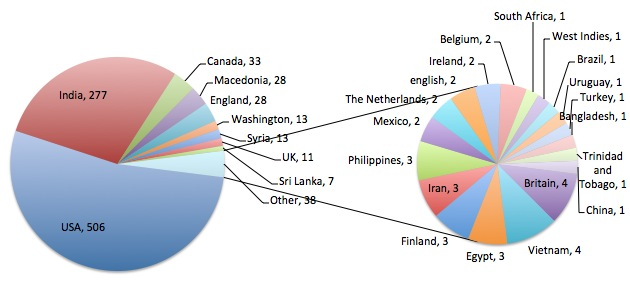
\includegraphics[width=150mm]{responsesPerCountry.jpg}
\captionfonts
\caption[Responses Per Country]{ Our user study primarily polled people from the United States and India, as can be seen by the number of responses originating from each country. }
\label{fig:responsesPerCountry}
\end{figure}

\begin{table}
\begin{center}

\begin{tabular}{|c|c|c|}
\hline 
Response By Country   &   Num Responses   \\ \hline
USA   &   489   \\ \hline
India   &   239   \\ \hline
England   &   37   \\ \hline
Canada   &   35   \\ \hline
UK   &   7   \\ \hline
Macedonia   &   14   \\ \hline
Egypt   &   4   \\ \hline
Belgium   &   3   \\ \hline
The Netherlands   &   3   \\ \hline
Mexico   &   3   \\ \hline
Finland   &   3   \\ \hline
Ireland   &   2   \\ \hline
Sri Lanka   &   7   \\ \hline
Bangladesh   &   1   \\ \hline
China   &   1   \\ \hline
Trinidad and Tobago   &   1   \\ \hline
Uruguay   &   1   \\ \hline
USA/Canada   &   1   \\ \hline
\end{tabular}

\captionfonts
\caption[Countries and responses]{ Here's a table with the number of responses per country}
\label{table:countryTally}
\end{center}
\end{table}



\chapter{Results}
\label{results}

\section{Phase One Results}
\label{results:userStudyPhaseOne}

In this phase, we recorded \uniqueUsersPhaseOneUserStudy users reciting any of the \numOronymsPhaseOneUserStudy  oronyms of the phrase ``an ice cold hour'', or any of the \numForthRightOohOronymPhrases oronyms for the phrase ``fourth rye to''.  Out of \numResponsesPhaseOneUserStudy recordings, only the recordings of the oronyms of ``fourth rye to" were found to diverge from our excepted phonetic patterns, likely due to poor microphone quality not being able to pick up the aspriated \emph{`f'} sound at the beginning of the phrase\cite{elko_electronic_2007}. All other oronyms were found to be within reasonable tolerance levels, with \recordingsPhaseTwoUserStudy recordings from one particular speaker found to be a close enough match to the general American accent to use his recordings in phase two.


\section{Phase Two Results}
\label{results:userStudyPhaseTwo}


We gathered \numTotalTranscriptionsPhaseTwo transcriptions for our \recordingsPhaseTwoUserStudy recorded phrases, with each recording garnering \numTranscriptionsPerRecordingPhaseTwoUserStudy transcriptions each.  Worldwide, the top four most-frequently transcribed phrases made up for 70\% of total transcriptions.  The top transcribed phrase worldwide was ``an ice cold hour'', with \phaseTwoUserStudyTimesTranscribedAnIceColdHour transcriptions, followed by  ``a nice cold hour'', with \phaseTwoUserStudyTimesTranscribedANiceColdHour transcriptions.  Following that, ``a nice gold hour'' had \phaseTwoUserStudyTimesTranscribedANiceGoldHour transcriptions, and ``in ice cold hour'' had \phaseTwoUserStudyTimesTranscribedInIceColdHour transcriptions. The breakdown of these top four can be seen in figure ~\ref{fig:mostCommonTranscriptionsPieChartGlobal} and table ~\ref{table:fullFreqVsActual}. 

All of the worldwide top transcribed phrases were predicted by our oronym-generator, except for ``a nice gold hour''.  This is a known limitation of our project, though, because we chose to focus on exact phonetic matches.  The cold/gold mishearing is a product of phoneme voiced/voiceless pair swapping, which we cover in-depth in section ~\ref{section:phonemeSwapping}. It is outside the current scope of our project. 


\begin{figure}
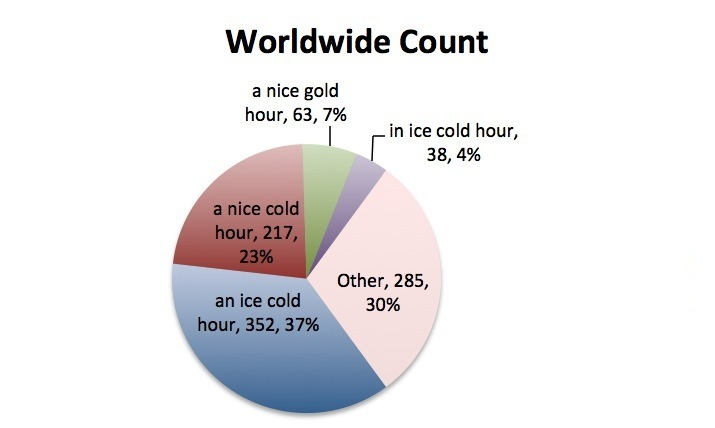
\includegraphics[width=150mm]{PieChart_WorldwideCount_noBar.jpg}
\captionfonts
\caption[Most Common Transcriptions Globally]{ Our top two transcriptions were ``a nice cold hour'' and ``an ice cold hour'' }
\label{fig:mostCommonTranscriptionsPieChartGlobal}
\end{figure}


\begin{table}
\begin{center}
\begin{tabular}{ | l | l | l | c | }
\hline 
predicted freq & phrase transcribed & total answers \\
\hline 
931028 &  an ice cold hour &  \phaseTwoUserStudyTimesTranscribedAnIceColdHour \\
\hline
7851662&   a nice cold hour &  \phaseTwoUserStudyTimesTranscribedANiceColdHour  \\
\hline
0  & a nice gold hour &  \phaseTwoUserStudyTimesTranscribedANiceGoldHour \\
\hline
5503158&   in ice cold hour &  \phaseTwoUserStudyTimesTranscribedInIceColdHour \\
\hline
0 &  an ice gold hour &  \phaseTwoUserStudyTimesTranscribedAnIceGoldHour \\
\hline
859307 &  an eye scold hour &  \phaseTwoUserStudyTimesTranscribedAnEyeScoldHour \\
\hline 
\end{tabular}
\captionfonts
\caption[Phrase word frequency sum vs times transcribed]{ In this table, we list all oronyms that were transcribed more than five times. Out of this list, all but the two containing the word ``gold" were predicted by our oronym algorithm.  However, we expected that any voiced/voiceless phoneme substitutions, like ``cold''/``gold'' would be missed by our algorithm. }
\label{table:fullFreqVsActual}
\end{center}
\end{table}


%\begin{figure}
%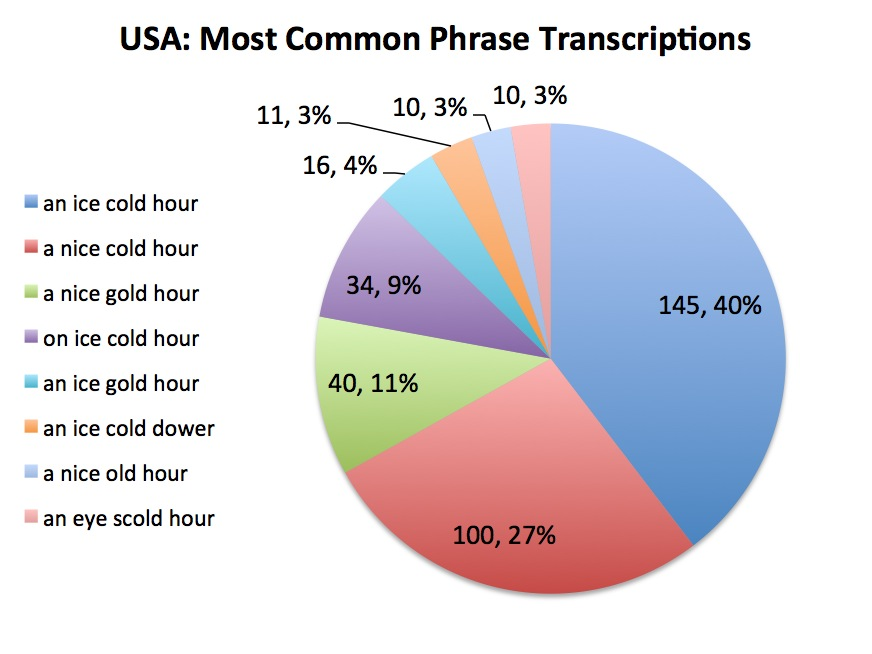
\includegraphics[width=150mm]{mostCommonTranscriptionsPieChartUSA.jpg}
%\captionfonts
%\caption[Most Common Transcriptions from American respondents]{ Though the breakdown is a bit different than the global transcription breakdown, you can still see the clear trend of ``a nice cold hour" and ``an ice cold hour" being the most common.  There is a slightly larger gap between these two phrase, we hypothesize, because the American transcribers are familiar with what words normally are in proximity to others. }
%\label{fig:mostCommonTranscriptionsPieChartUSA}
%\end{figure}



\subsection{Transcribed oronyms' observed frequency vs expected frequency}
\label{results:transcriptionExpectedVsObservedFreq}

Though the most commonly transcribed phrases were predicted by our method of oronym generation, figure ~\ref{fig:results:aNiceColdHourObserved} shows an unexpected distribution of the number of times each phrase was transcribed versus the frequency metric that we calculated. We hypothesized that a simple summation of the UNISYN-provided word frequencies for each word in a phrase would produce a meaningful indicator of whether a phrase's likelyhood to be heard.  

\begin{figure}
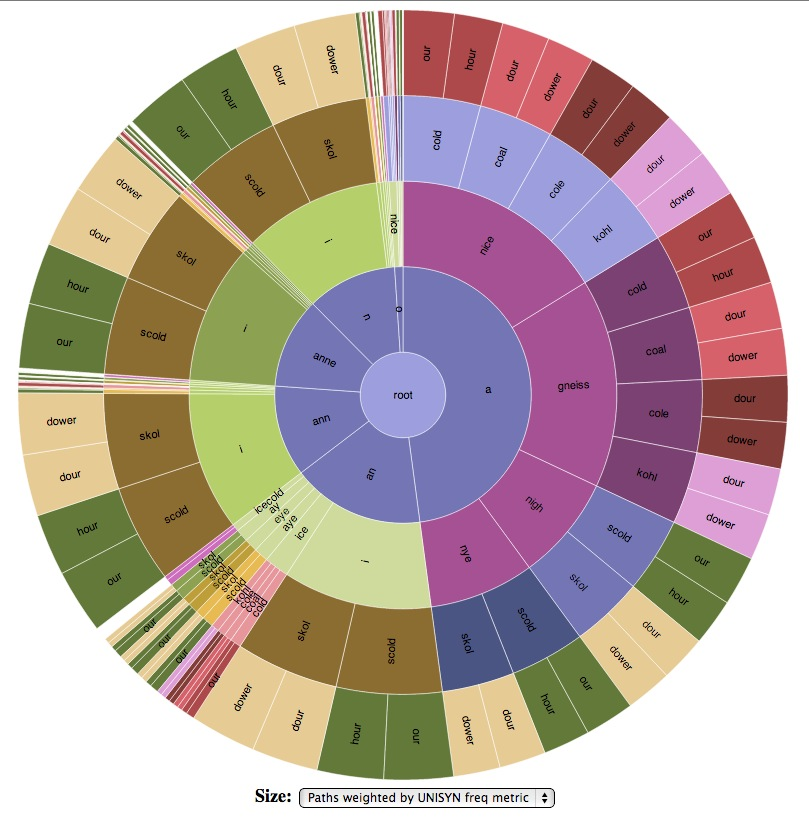
\includegraphics[width=150mm]{aNiceColdHour_UNISYN_FreqMetric_withUnpredictedSliver.jpg}
\captionfonts
\caption[Sunburst Chart for A Nice Cold Hour using UNISYN metrics for comparison to observed frequency sunburst]{Sunburst Chart for A Nice Cold Hour using UNISYN metrics for comparison to observed frequency sunburst}
\label{fig:results:aNiceColdHourUNISYNwithUnpredicted}
\end{figure}

\begin{figure}
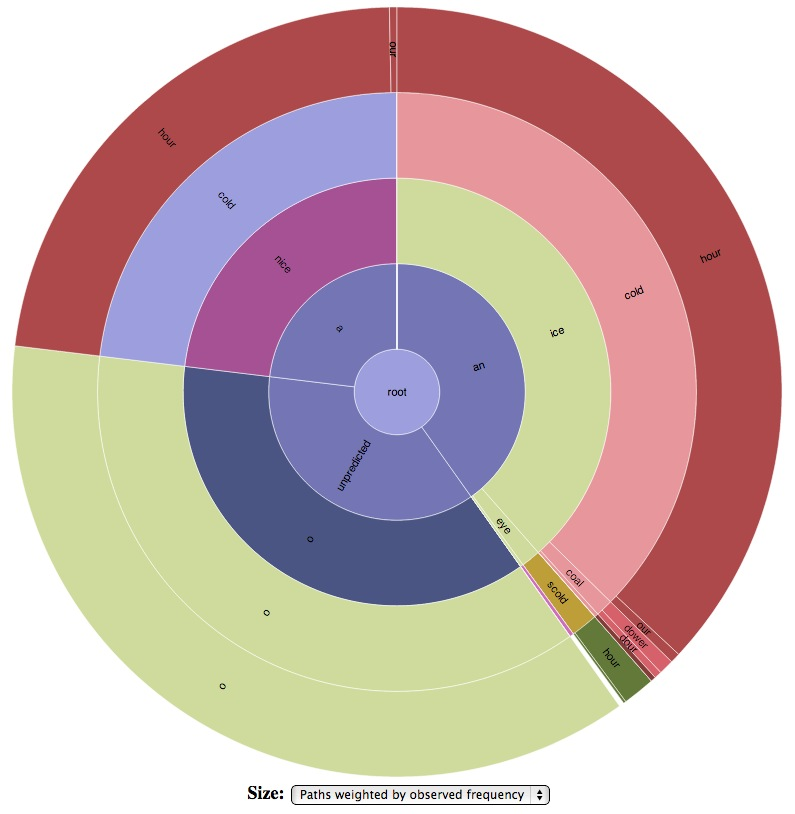
\includegraphics[width=150mm]{aNiceColdHour_Observed.jpg}
\captionfonts
\caption[Sunburst Chart for A Nice Cold Hour using observed frequencies]{Sunburst Chart for A Nice Cold Hour using observed frequencies}
\label{fig:results:aNiceColdHourObserved}
\end{figure}


Unfortunately, that proved not to be the case.  In figure ~\ref{fig:results:aNiceColdHourUNISYNwithUnpredicted}, we see the sunburst diagram for the expected distribution of transcribed phrases based upon the UNISYN frequency metric that we calculated.  In figure ~\ref{fig:results:aNiceColdHourObserved}, we see the sunburst diagram for the transcriptions we observed, with a special slice representing all the transcriptions we did not predict. The unpredicted slice is nearly as large as the slice for ``an ice cold hour'', which was observed the most often out of all expected transcriptions. 


\subsection{Statistical measurement of expected versus observed transcription frequency}
\label{results:statisticsINYOURFACE}


A statistical analysis of the observed dataset versus the expected dataset, using a one-proportion z test, further proves that the calculated UNISYN frequency values were not a good predictor of observed transcription.   Using the top two observed transcriptions as our sample population, we take a look at the phrases \phraseOne and \phraseTwo.  The phrase \phraseOne has a calculated UNISYN freq metric of \unisynFreqForPhraseOne, and had \USATranscriptionsOfPhraseOne actual transcriptions observed among people living in the United States. The phrase \phraseTwo has a calculated UNISYN freq metric of \unisynFreqForPhraseTwo, and had \USATranscriptionsOfPhraseTwo actual transcriptions observed among people living in the United States. Therefore, the expected population is \unisynCombinedFreq, and the observed population is \USACombinedTranscriptions.  

Given those population, the expected population proportion for \phraseOne would be \unisynFreqForPhraseOne  $\div$ \unisynCombinedFreq, or \expectedProportionOfPhraseOneOccurances.  

In our user study, we found that \USATranscriptionsOfPhraseOne people transcribed \phraseOne, and \USATranscriptionsOfPhraseTwo people transcribed \phraseTwo, for a ratio of 0.65 to 1, where \phraseOne accounts for 39.56\% ( p = \observedProportionOfPhraseOneOccurances ) of the combined count. 

Given the observed population proportion of \observedProportionOfPhraseOneOccurances and the expected population proportion \expectedProportionOfPhraseOneOccurances, we did a one-proportion z test with an $\alpha$ of \alphaSigFigs.  The z value returned was \UNISYNzVal, meaning that the observed population proportion was \UNISYNzVal standard deviations away from the expected population proportion.  When we used this z value to compute a p value, we got a value so low that we were unable find a calculator with enough decimal places to show it without rounding it to zero.

In short, the per-occurance frequency metric predictions derived from UNISYN don't even remotely match the observed data.


The below is here mostly for my edification: (I'll delete it when my edits are all done.)

Givens for Phrase (1) (\phraseOne) :

Calculated metric: \unisynFreqForPhraseOne

Actual count: x = \USATranscriptionsOfPhraseOne


Givens for Phrase (2) (\phraseTwo) :

Calculated metric: \unisynFreqForPhraseTwo

Actual count: x = \USATranscriptionsOfPhraseTwo

$\alpha$ = significance Level = \alphaSigFigs

Calculated sum: \unisynFreqForPhraseOne + \unisynFreqForPhraseTwo =  \unisynCombinedFreq

Actual sum: \USATranscriptionsOfPhraseOne + \USATranscriptionsOfPhraseTwo = \USACombinedTranscriptions

p = population proportion of \phraseOne occurrences

p = \unisynFreqForPhraseOne   $\div$  \unisynCombinedFreq  = \pvalue 

$H_{o}$ :  p = \pvalue 
$H_{a}$ :  p $\neq$ \pvalue 

Actual: 
\USATranscriptionsOfPhraseOne  $\div$ \USACombinedTranscriptions  = 

1-proportion z-test

z = \UNISYNzVal std deviations away from expected.

If pvalue < $\alpha$, reject $H_{o}$

pvalue $\approx$ 0 < \alphaSigFigs

So, reject $H_{o}$


\subsection{Observations on Transcription Count per Recording for each transcribed phrase}
\label{results:transcriptionCountPerRecording}

The Transcription Count by Recording graphs show how many occurances of a certain transcription were produced from each recording. Each graph represents one transcription, and has bars for each recording, where each bar shows how many times the transcription was observed for that particular recording. The graph also compares the observed incidences of those transcriptions with the expected UNISYN frequency metric. The X axis lists the transcribed phrase.  The right Y axis corresponds to the smaller, multi-colored bars. Each bar represents the number of times that a transcribed phrase was observed for that particular recording. 
The left X axis corresponds to the large blue bar behind the smaller bars. The blue bar represents the calculated UNISYN frequency metric for the transcription.


When you compare the bars from the two y axes, some interesting patterns appear. 

\subsubsection{An ice cold hour}
\label{results:transcriptionCountPerRecording:an_ice_cold_hour}

When looking at figure ~\ref{fig:results:transcriptionCountPerRecordingAnIceColdHour}, we notice that all but 12 out of the 362 transcriptions of ``an ice cold hour'' come from recordings of phrases that similarly begin with ``an''. This suggests the existence of some un-measured value related to pronunciation that makes the theoretically identical phonetic sequences of ``an ice cold hour'' and ``a nice cold hour'' be heard as functionally different. Also, note that in figure ~\ref{fig:results:transcriptionCountPerRecordingAnIceColdHour}, the blue bar representing the UNISYN frequency prediction for the transcribed phrase underpredicts the number of transcriptions from recordings that begin with ``an'', while doing a fairly good job of predicting transcription incidence for recordings that begin with ``a''.


\begin{figure}
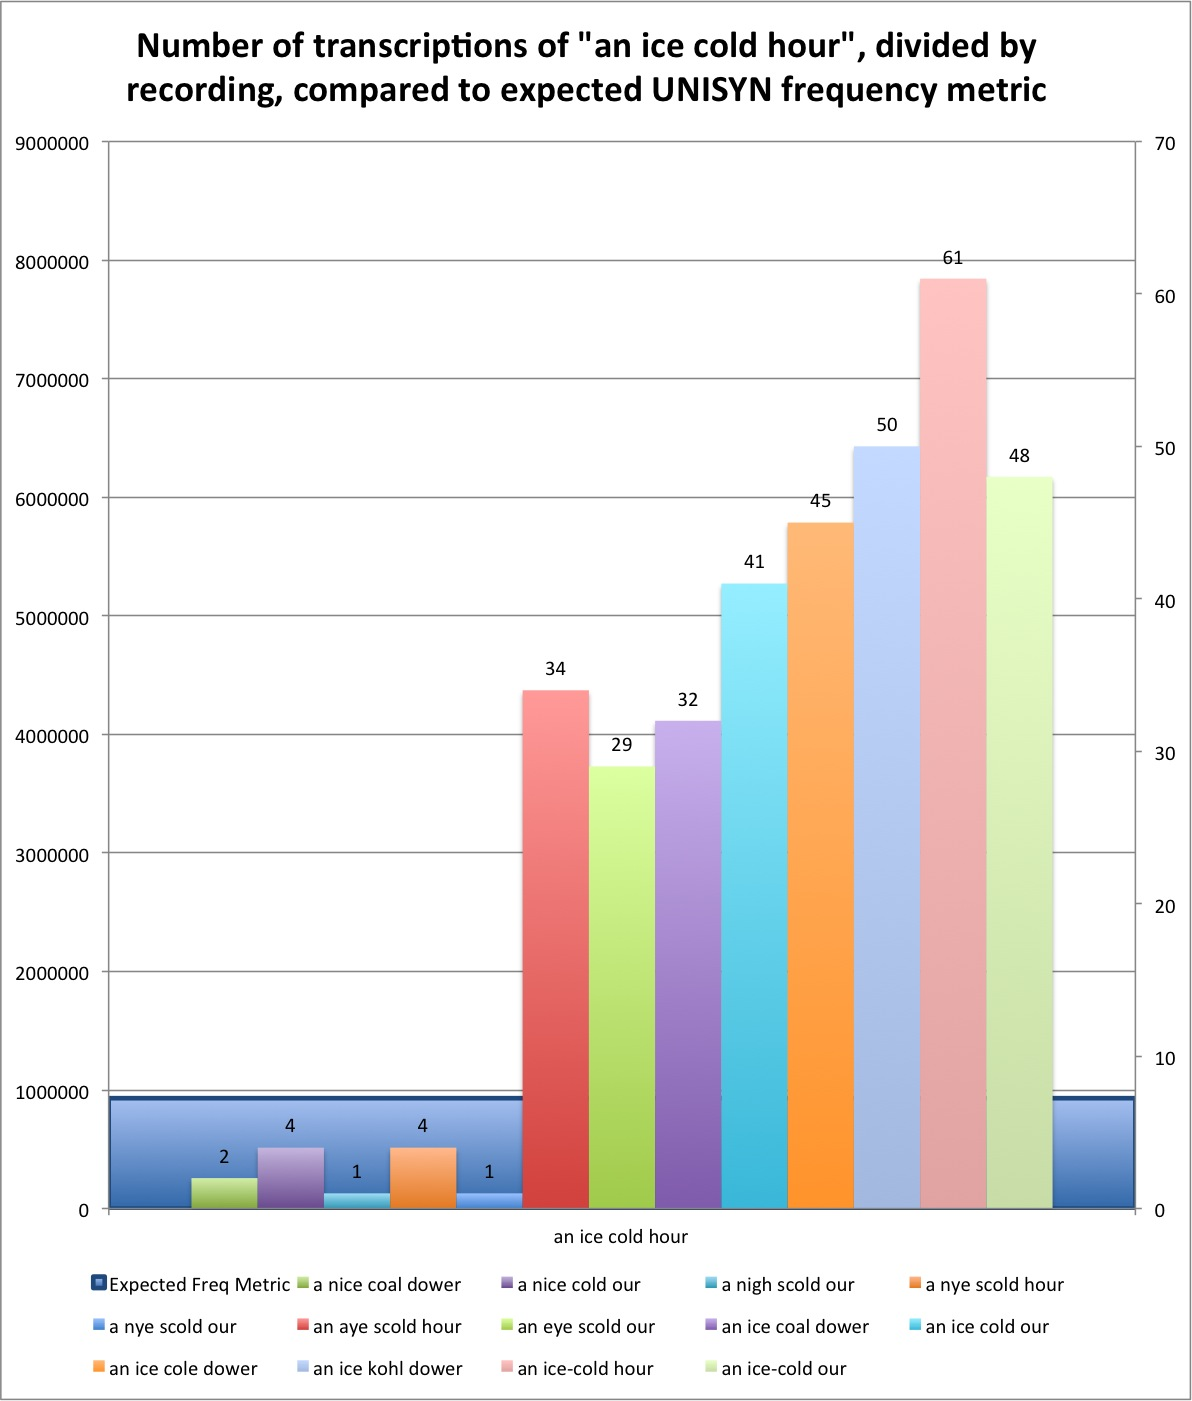
\includegraphics[width=\textwidth]{TranscriptionCountPerRecording_an_IceColdHour.jpg}
\captionfonts
\caption[Transcription Count Per Recording for the transcribed phrase ``an ice cold hour'']{ This graph represents all transcriptions of the phrase ``an ice cold hour'', divided into columns based on what recording were transcribed as ``an ice cold hour''. The large blue bar in the background shows the predicted frequency metric for the phrase in question.}
\label{fig:results:transcriptionCountPerRecordingAnIceColdHour}
\end{figure}

\subsubsection{A nice cold hour}
\label{results:transcriptionCountPerRecording:a_nice_cold_hour}

In figure ~\ref{fig:results:transcriptionCountPerRecordingANiceColdHour}, we see that, while most of the transcriptions of ``a nice cold hour'' came from recordings of phrases that begin with 'a', a not-inconsiderable number came from the recordings for the phrases ``an ice cold our'' and ``an ice-cold our''. When taken in regards to the conclusions we drew from figure ~\ref{fig:results:transcriptionCountPerRecordingAnIceColdHour} in section ~\ref{results:transcriptionCountPerRecording:an_ice_cold_hour}, we can conclude that, while listeners appear not to be able to hear an `a' as an `an', listeners can, under certain circumstances, hear an `an' as an `a'.  The blue prediction bar shows that the expected incidence over all recordings was much higher than the observed incidence, and only came close to being correct for the recorded phrases ``a nice cold hour'' and ``a nice coal dower''.

\begin{figure}
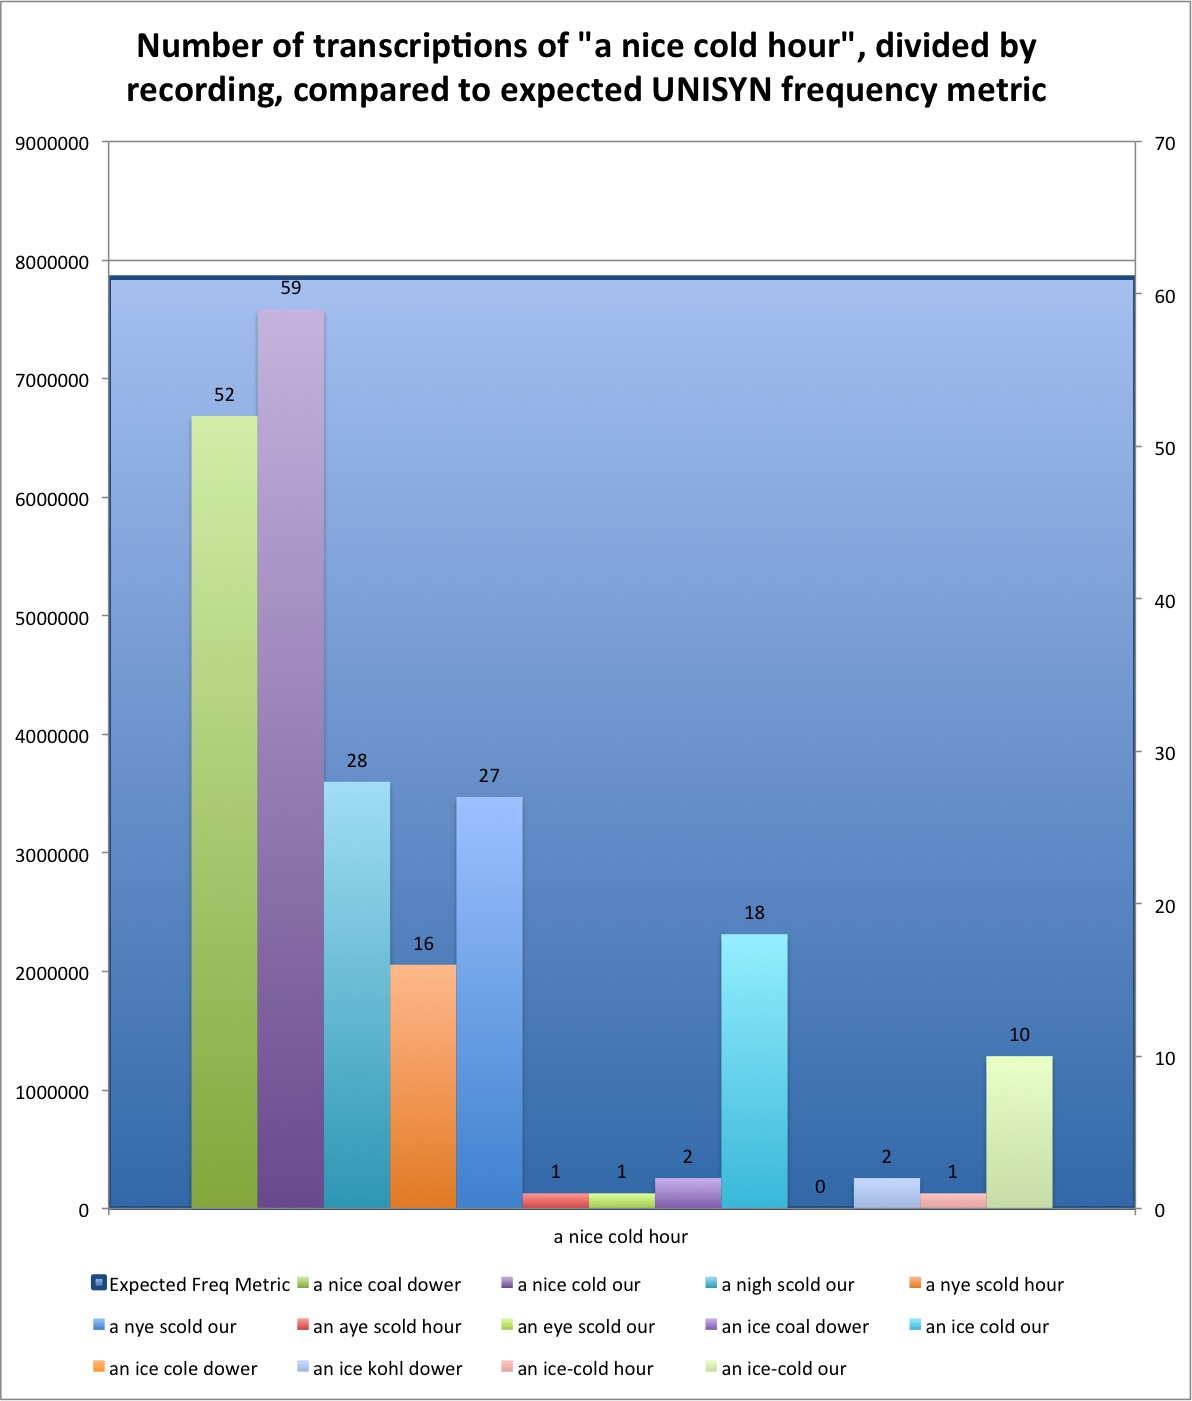
\includegraphics[width=\textwidth]{TranscriptionCountPerRecording_a_NiceColdHour.jpg}
\captionfonts
\caption[Transcription Count Per Recording for the transcribed phrase ``a nice cold hour'']{ This graph represents all transcriptions of the phrase ``a nice cold hour'', divided into columns based on what recording were transcribed as ``a nice cold hour''. The large blue bar in the background shows the predicted frequency metric for the phrase in question.}
\label{fig:results:transcriptionCountPerRecordingANiceColdHour}
\end{figure}



\subsubsection{In ice cold hour}
\label{results:transcriptionCountPerRecording:in_ice_cold_hour}

This chart in figure ~\ref{fig:results:transcriptionCountPerRecordingInIceColdHour} is for the third most common transcription, ``in ice cold hour''.  Transcriptions of this phrase are fairly evenly distributed among the recordings, though there is a spike of transcriptions on  ``an ice-cold hour''.  Additionally, similar to earlier observations, the transcriptions occur a lot less frequently than the UNISYN frequency metric bar suggests they should.

\begin{figure}
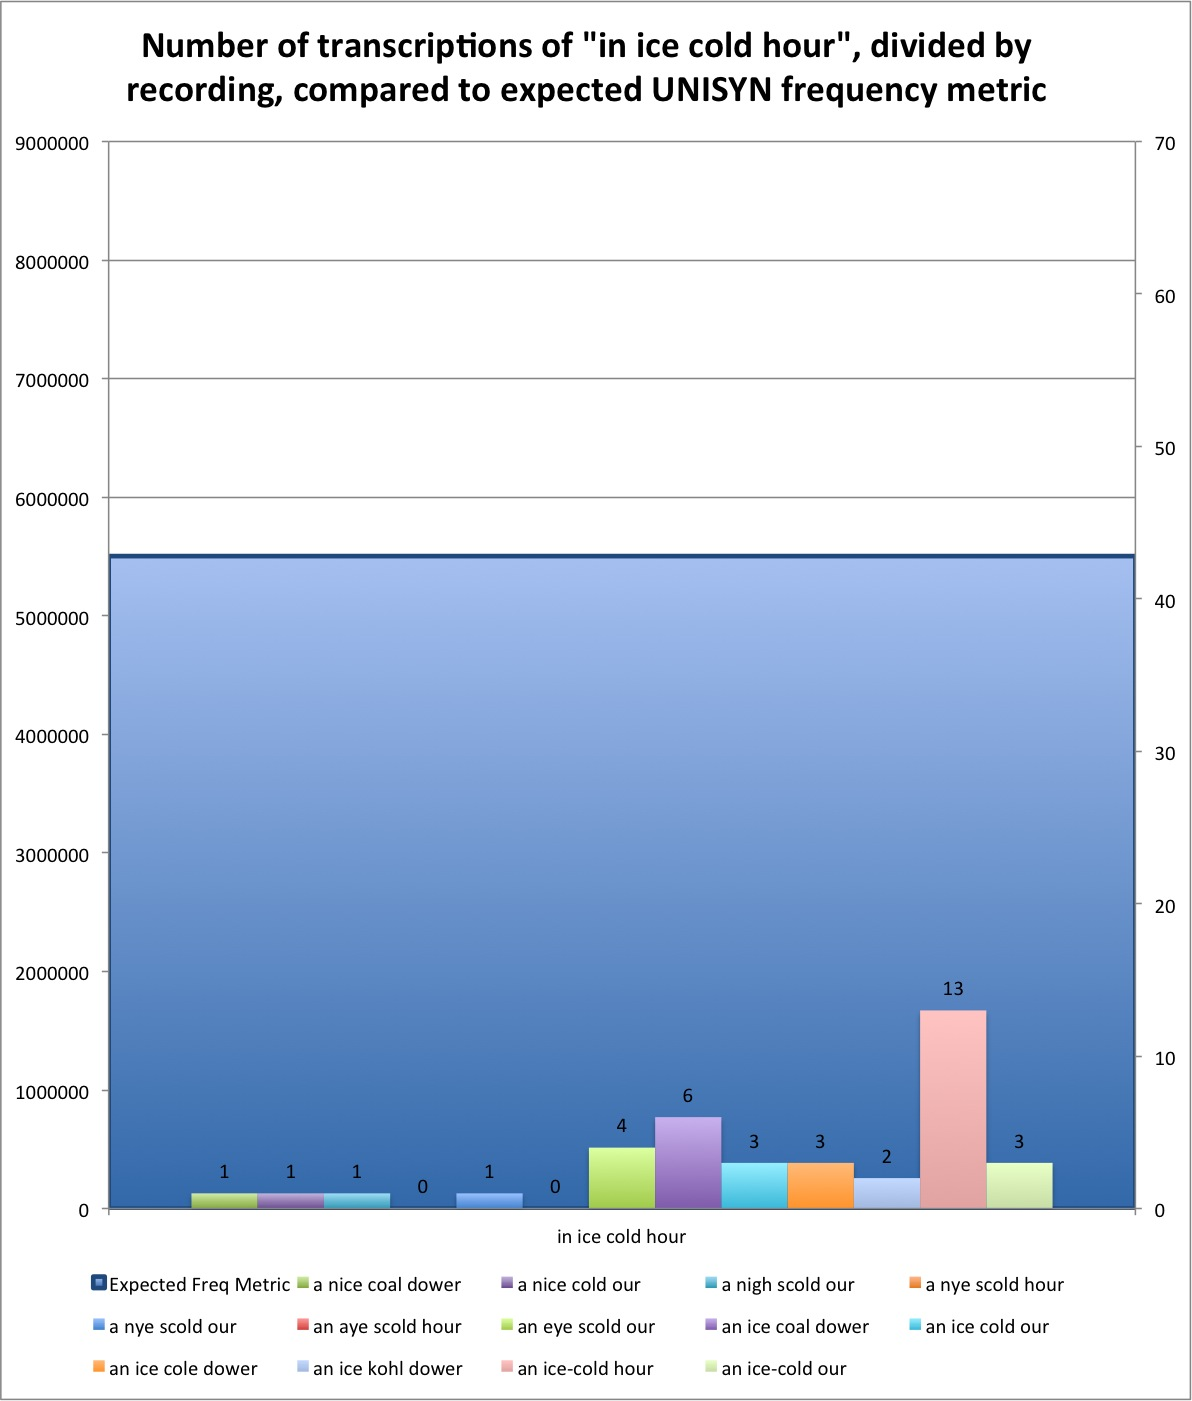
\includegraphics[width=\textwidth]{TranscriptionCountPerRecording_inIceColdHour.jpg}
\captionfonts
\caption[Transcription Count Per Recording for the transcribed phrase ``in ice cold hour'']{ This graph represents all transcriptions of the phrase ``in ice cold hour'', divided into columns based on what recording were transcribed as ``in ice cold hour''. The large blue bar in the background shows the predicted frequency metric for the phrase in question.}
\label{fig:results:transcriptionCountPerRecordingInIceColdHour}
\end{figure}



\subsubsection{A nice gold hour}
\label{results:transcriptionCountPerRecording:a_nice_gold_hour}

The chart in figure ~\ref{fig:results:transcriptionCountPerRecordingANiceGoldHour} for the transcriptions of ``a nice gold hour'' shows that the source recordings of those transcriptions are very specific: only the recordings of ``a nye scold our'', ``a nye scold hour'', and ``a nigh scold our'' produce the 'g'/'c' substitution. In fact, all of our transcriptions that involved the word ``gold'' arose from these recordings. This suggests a relationship between the phonemes \texttt{s k} and \texttt{g}, and warrants further investigation, as suggested later in section ~\ref{section:phonemeSwapping}. As shown by the lack of a background blue bar in this diagram, this transcription was not predicted by our oronym generation algorithm, due to the aforementioned phoneme swapping.

\begin{figure}
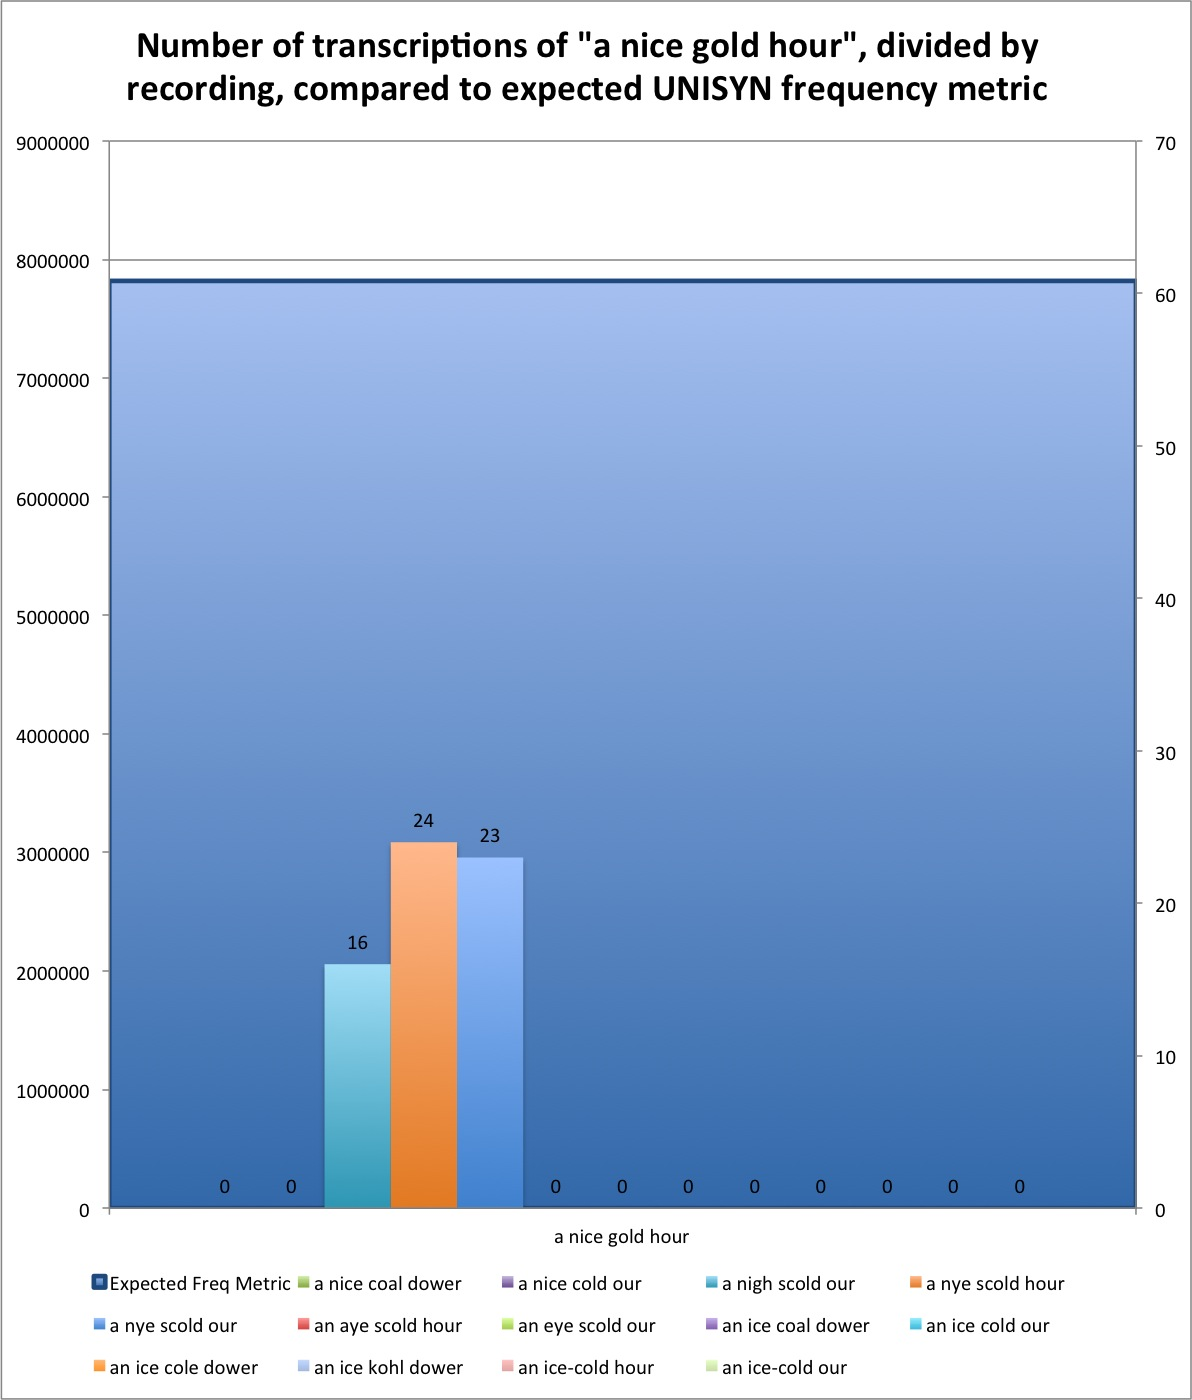
\includegraphics[width=\textwidth]{TranscriptionCountPerRecording_aNiceGoldHour.jpg}
\captionfonts
\caption[Transcription Count Per Recording for the transcribed phrase ``a nice gold hour'']{ This graph represents all transcriptions of the phrase ``a nice gold hour'', divided into columns based on what recording were transcribed as ``a nice gold hour''. The large blue bar in the background shows the predicted frequency metric for the phrase in question.}
\label{fig:results:transcriptionCountPerRecordingANiceGoldHour}
\end{figure}


\subsubsection{An ice cold dower}
\label{results:transcriptionCountPerRecording:an_ice_cold_dower}

Figure ~\ref{fig:results:transcriptionCountPerRecordingANiceColdDower} shows the transcriptions for the phrase ``an ice cold dower''. This phrase features repeated-phoneme auto-deletion or auto-insertion. Repeated-phoneme auto-deletion or -insertion occurs when two identical and adjacent phonemes are blurred into one sound.  This can result in the listener putting two phonemes where only one exists (as in this case), or putting one phoneme where two exist. This phenomenon, while known to us, is outside the scope of the current project, and suggested for future work.  Due to this limit in scope, this transcription was not predicted by our oronym generation algorithm, as shown by the lack of a background blue frequency prediction bar in figure ~\ref{fig:results:transcriptionCountPerRecordingANiceColdDower}.

\begin{figure}
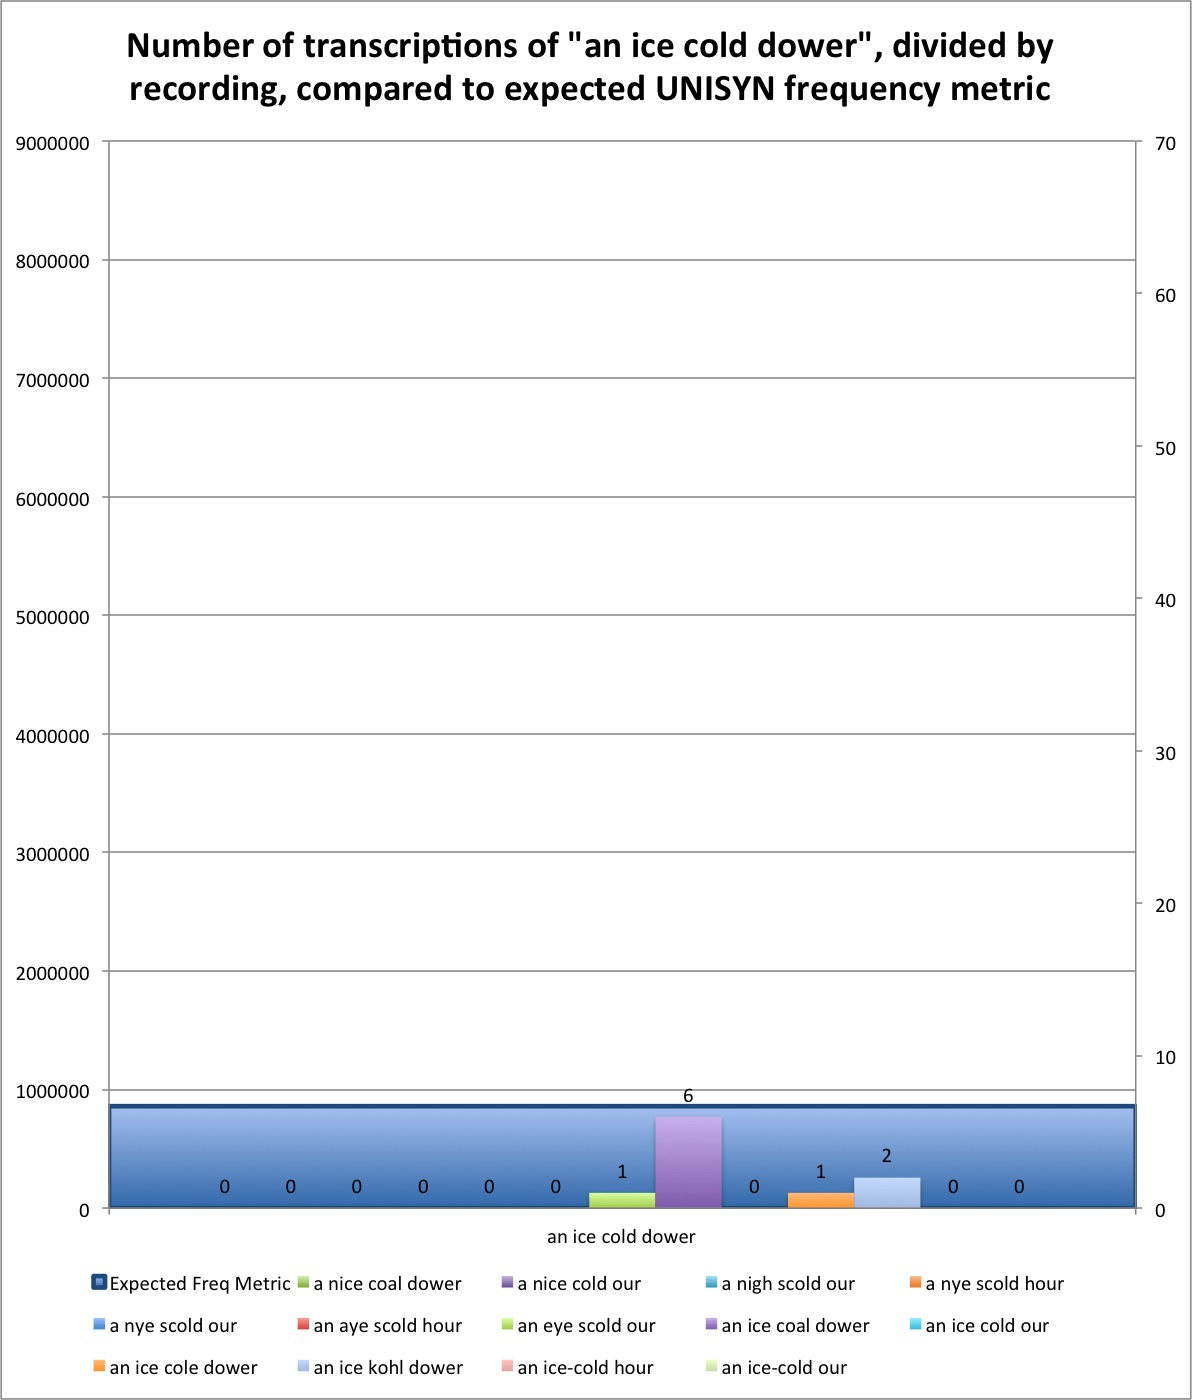
\includegraphics[width=\textwidth]{TranscriptionCountPerRecording_anIceColdDower.jpg}
\captionfonts
\caption[Transcription Count Per Recording for the transcribed phrase ``a nice cold dower'']{ This graph represents all transcriptions of the phrase ``a nice cold dower'', divided into columns based on what recording were transcribed as ``a nice cold dower''. The large blue bar in the background shows the predicted frequency metric for the phrase in question.}
\label{fig:results:transcriptionCountPerRecordingANiceColdDower}
\end{figure}


\subsubsection{An eye scold hour}
\label{results:transcriptionCountPerRecording:an_eye_scold_hour}

The chart for ``an eye scold hour'', shown in figure ~\ref{fig:results:transcriptionCountPerRecordingAnEyeScoldHour}, is primarily interesting in that it appears more or less deterministically interpretable. The only recordings that resulted in this phrase were those for ``an eye scold hour'' or ``an aye scold hour''. We hypothesize that this has something to do with word emphases, and suggest investigating this for future work. Interestingly enough, the predicted frequency value (scaled) was fairly close to the actual occurance for that phrase.


\begin{figure}
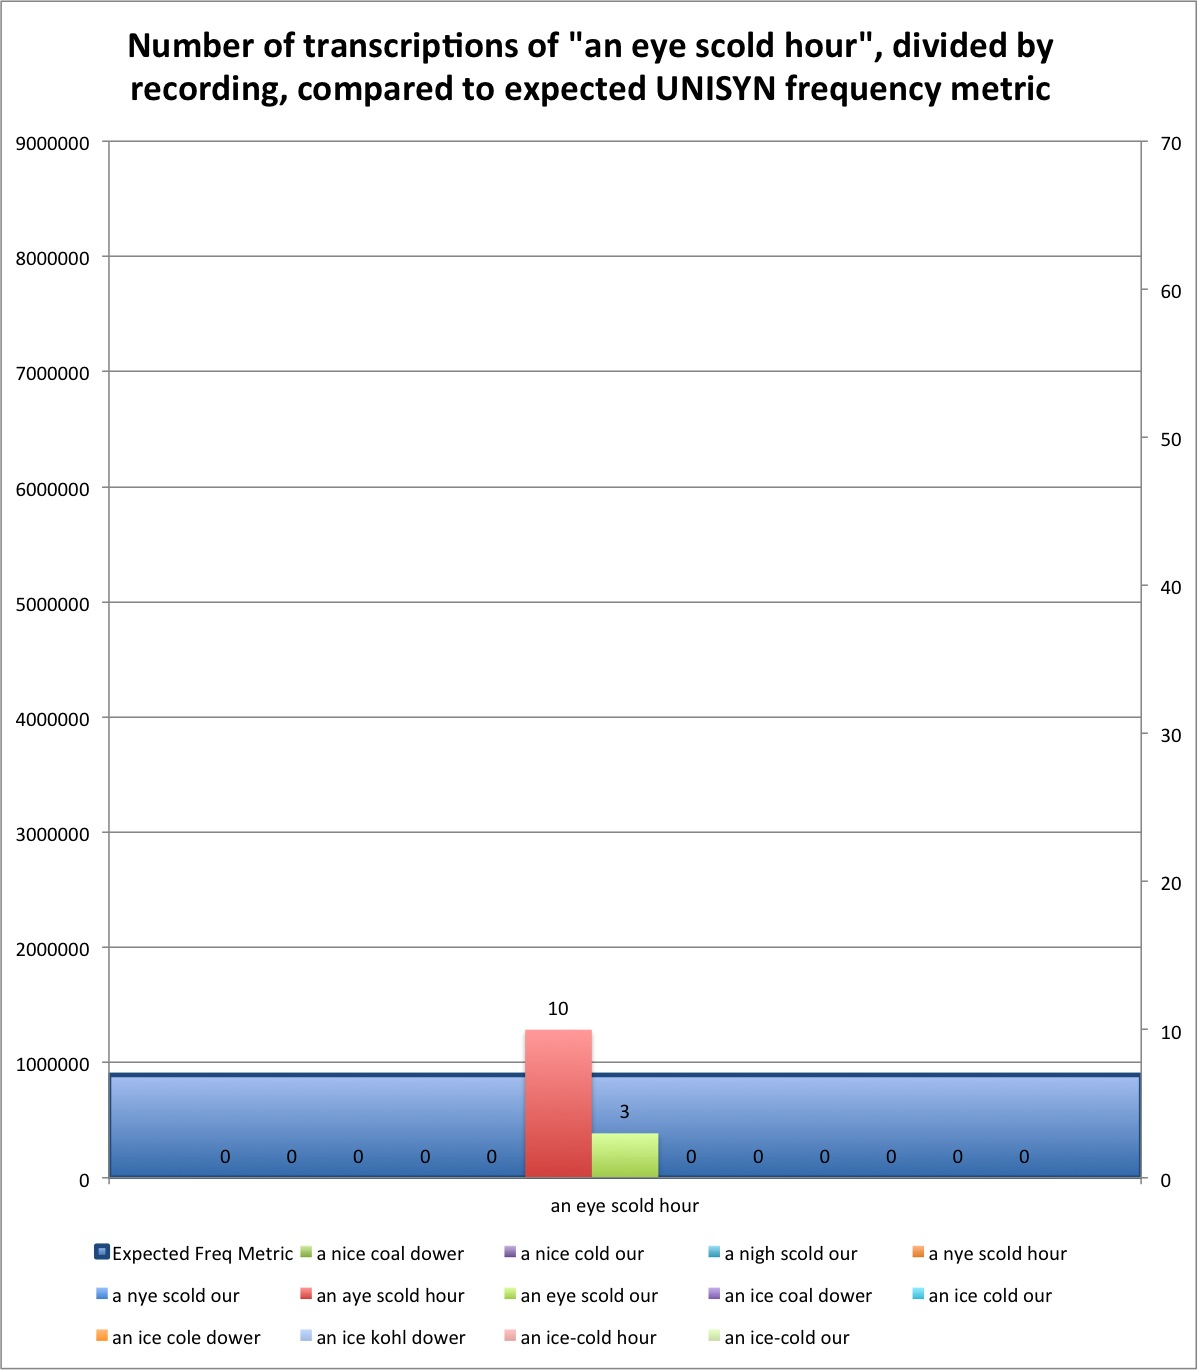
\includegraphics[width=\textwidth]{TranscriptionCountPerRecording_anEyeScoldHour.jpg}
\captionfonts
\caption[Transcription Count Per Recording for the transcribed phrase ``an eye scold hour'']{ This graph represents all transcriptions of the phrase ``an eye scold hour'', divided into columns based on what recording were transcribed as ``an eye scold hour''. The large blue bar in the background shows the predicted frequency metric for the phrase in question.}
\label{fig:results:transcriptionCountPerRecordingAnEyeScoldHour}
\end{figure}

\subsubsection{An ice coal dower}
\label{results:transcriptionCountPerRecording:an_ice_coal_dower}

The chart for ``an ice coal dower'' in figure ~\ref{fig:results:transcriptionCountPerRecordingAnIceCoalDower} is notable in that all its transcriptions came from recordings that began in ``an'' and ended in ``dower'', like the phrase itself does. As in ~\ref{fig:results:transcriptionCountPerRecordingAnEyeScoldHour}, we suggest that the near-deterministic interpretation has something to do with emphases, and suggest investigating this for future work. The UNISYN frequency metric once again predicted higher expected incidences than were actually observed for this transcription.

\begin{figure}
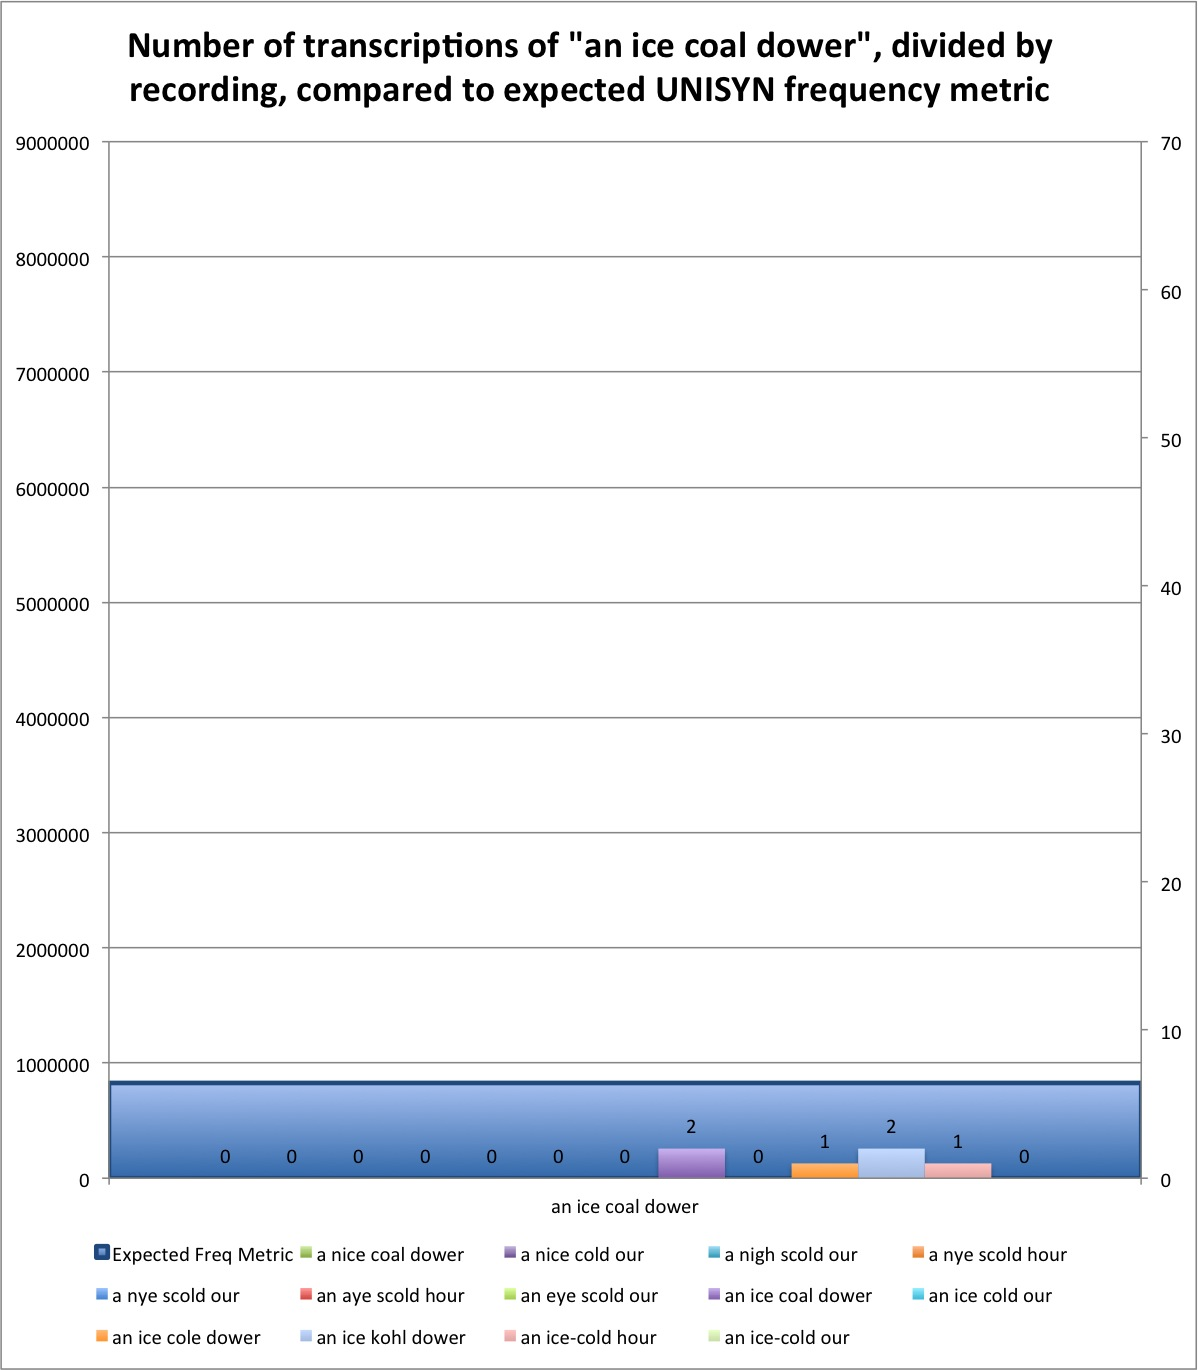
\includegraphics[width=\textwidth]{TranscriptionCountPerRecording_anIceCoalDower.jpg}
\captionfonts
\caption[Transcription Count Per Recording for the transcribed phrase ``an ice coal dower'']{ This graph represents all transcriptions of the phrase ``an ice coal dower'', divided into columns based on what recording were transcribed as ``an ice coal dower''. The large blue bar in the background shows the predicted frequency metric for the phrase in question.}
\label{fig:results:transcriptionCountPerRecordingAnIceCoalDower}
\end{figure}







\subsection{Transcription Breakdown By Country}
\label{results:transcriptionsByCountry}


When comparing transcriptions from countries where English is the dominant language (as shown in figure ~\ref{fig:results:EnglishDominantPieChart}) to those from countries where it is not (as shown in figure ~\ref{fig:results:NonNativePieChart}), we can make some interesting observations.  

\begin{figure}
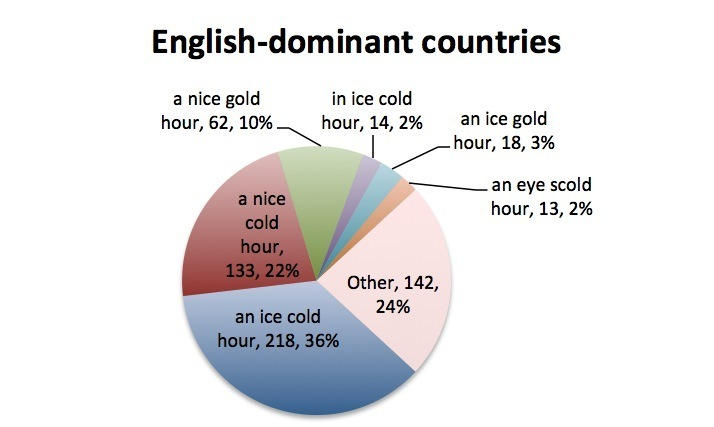
\includegraphics[width=\textwidth]{PieChart-EnglishDominantCountries-nobar.jpg}
\captionfonts
\caption[Pie Chart of transcriptions from countries that are primarily English-speaking]{ Pie Chart of transcriptions from countries that are primarily English-speaking.}
\label{fig:results:EnglishDominantPieChart}
\end{figure}

\begin{figure}
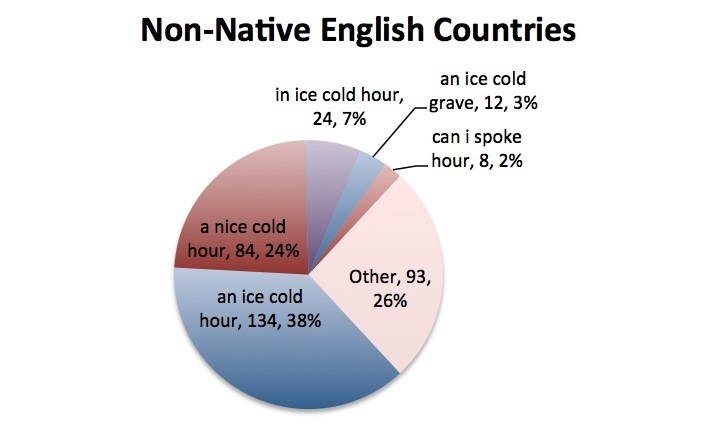
\includegraphics[width=\textwidth]{PieChart-NonNativeEnglishCountries-nobar.jpg}
\captionfonts
\caption[Pie Chart of transcriptions from countries that are Non-native English speakers]{ Pie Chart of transcriptions from countries that are Non-native English speakers.}
\label{fig:results:NonNativePieChart}
\end{figure}

\begin{enumerate}

\item The most common transcription for both is ``an ice cold hour'', with \percentTranscriptionsPerCountryAnIceColdHourEnglishDominant\% native-speaker transcriptions ( \transcriptionsPerCountryAnIceColdHourEnglishDominant) and \percentTranscriptionsPerCountryANiceColdHourNonNative\% non-native ( \transcriptionsPerCountryAnIceColdHourNonNative).

\item The second most common transcription is also the same for both (``a nice cold hour''), but it accounts for a larger percentage of the non-native pie ( \percentTranscriptionsPerCountryANiceColdHourNonNative\% compared to the native \percentTranscriptionsPerCountryANiceColdHourEnglishDominant\% ).

\item The third most common transcription differs for native and non-native speakers. 

Native speakers transcribed ``a nice gold hour'' \transcriptionsPerCountryANiceGoldHourEnglishDominant times, accounting for \percentTranscriptionsPerCountryANiceGoldHourEnglishDominant\% of all native transcriptions. In comparison, only \transcriptionsPerCountryANiceGoldHourNonNative non-native speaker transcribed that phrase, for a measley \percentTranscriptionsPerCountryANiceGoldHourNonNative\% of total non-native transcriptions. 

This brings up an interesting data point---the third most popular transcription for native speakers barely shows up at all for non-native transcribers. There may be something about common phoneme substitution that native speakers pick up on that non-natives do not; specifically, a cold/gold merger.  

 The third most common transcription for non-native speakers is ``in ice cold hour'', which was transcribed \transcriptionsPerCountryInIceColdHourNonNative times, and makes up \percentTranscriptionsPerCountryInIceColdHourNonNative\% of non-native transcriptions.  This phrase was the fifth most common transcription for native speakers, with \transcriptionsPerCountryInIceColdHourEnglishDominant transcriptions making up \percentTranscriptionsPerCountryInIceColdHourEnglishDominant\% of total transcriptions.  

\item The fourth most common transcription for native speakers was ``an ice gold hour'', getting \percentTranscriptionsPerCountryAnIceGoldHourEnglishDominant\% of the total with \transcriptionsPerCountryAnIceGoldHourEnglishDominant transcriptions (by 14 unique transcribers).  This phrase was not transcribed by any non-native speakers. This exhibits the same phone/phoneme substitution that we saw with ``a nice gold hour''.

The fourth most common phrase for non-native speakers, ``an ice cold grave'', was only transcribed by one unique worker, and as such, is not going to be taken into serious consideration. The fifth most common phrase, ``can I spoke hour'', was also only transcribed by one unique worker, and so also cannot be taken into serious consideration.


\end{enumerate}



\chapter{Future Work}
\label{futureWork}

\section{Deficiencies in The Oronyminator}
\label{section:directImprovementsToMisheardMeOronymParseTree}

In some cases, our expected, UNISYN-derived phrase-frequency metric did not accurately line up with the observed transcription frequencies from our user studies.  We believe that there are several possible reasons for this.  

\subsection{Frequency Validity}
\label{subsection:frequencyValidity}
Our frequency source data from UNISYN ended up being less than statisfactory, due to several factors, deliniated below. 

\subsubsection{Corpus Composition deficiencies}
\label{futureWork:frequency:CorpusCompositionDeficiencies}

The lack of quality phonemic frequency data is a known defeciency in our source dictionary, UNISYN. According to the authors of the UNISYN lexicon documentation:
\begin{quote}
It should be noted that the frequency field, as it was obtained from simple word lists, is \emph{not particularly reliable} (emphasis mine).\cite{fitt_documentation_2000}  
\end{quote}
The UNISYN frequency count is based upon a large but not exhaustive corpus of text.  It has some particularly glaring deficiencies in the medical arena.  We find this frustrating, because knowledge about common medical mondegreens could be used to prevent mistakes in patient's treatment plans\cite{medicalMondegreensWhenIUseAWord}. Also, it meant that the word ``colitis'' wasn't in our dictionary, and we therefore couldn't use the example ``the girl with colitis goes by''/``the girl with kaleidescope eyes''. 


\subsubsection{Homograph Differentiation}
\label{futureWork:frequency:HomographDifferentiation}


Additionally, our source frequency data cannot and does not distinguish between words that may be homographs (that is, words that sound different but are spelled the same). This makes our program improperly weight some phrases over others. 

For example, take the words for the animals ``bucks'' and ``does''.  ``Bucks'' has a frequency of 1133, and ``does'' has a frequency of 508386.  For comparison, ``deer'' has a frequency of 1896.  You can see the relative scale of these in figure ~\ref{fig:DoesBucksDeerBubbleGraph}.  It seems highly unlikely that the male and female labels for a species would be as or more common than the actual name of the species, given that we don't see this for sheep (sheep at 13572 , ewe at 186 ,and  ram at 681) or horses (horse at 27559 , mare at 1055 , and stallion at 644 ).  What is much more likely is that ``bucks'' is getting extra hits through its meaning as a slang synonym for dollars (dollars at 8927), and ``does'' is getting most of its frequency count for the 3rd person present tense of the verb ``to do''.  That seems very likely, given that the frequency for the singular ``doe'' is only 1077. 

\begin{figure}
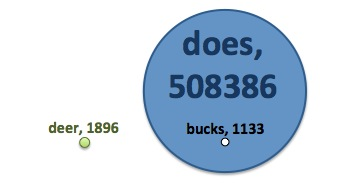
\includegraphics{DoesBucksDeerBubbleGraph.jpg}
\captionfonts
\caption[Bubble Chart comparison of Frequency for deer, does, and bucks]{Bubble Chart comparison of Frequency for deer, does, and bucks }
\label{fig:DoesBucksDeerBubbleGraph}
\end{figure}

Future work on our project would benefit from using a dictionary with some way of distinguishing homographs when counting frequency.


\subsubsection{Frequency Dictionary Tallying Methods}
\label{futureWork:frequency:freqDictTallyMethods}


In the future, we'd also like to use word frequency values from a dictionary that takes a larger, more-diverse dataset into its frequency count, such as the frequency lists from the Corpus of Contemporary American English\cite{freeFreqList}.  The COCA corpus is entirely focused on word frequency, and as such, does not contain any phonetic data.  However, it contains several different ways of determining frequency of words that overcome some of the shortcomings we ran into trying to compare the semantically-identical words `a' and `an'.  `A' is found much for frequently than `an', but both are just as common.  In the UNISYN dictionary, we only have contextless frequency counts.  In the COCA frequency dictionary, they keep two types of counts: one for how many times the word has been found total, and one for how many documents the word has been found in.  This way, even though `a' is found almost seven times as often than `a' overall, we know that they're equally-familiar words, because they are both found in approximately 160k corpus entries\cite{davies_word_2011}.

As a proof of concept, we created a sunburst diagram for ``an ice cold hour'' using COCA by-document frequency values (shown in figure ~\ref{fig:futureWork:COCAsunburst}), to compare it against the sunburst diagram created using UNISYN frequency values(shown in figure ~\ref{fig:futureWork:UNISYNsunburst}).  The COCA-based sunburst, while still inaccurate, at least has a ratio of phrases beginning with ``a'' to ``an'' that is closer to the actual observed ratio (which can be seen back in figure ~\ref{fig:results:aNiceColdHourObserved}).



\begin{figure}
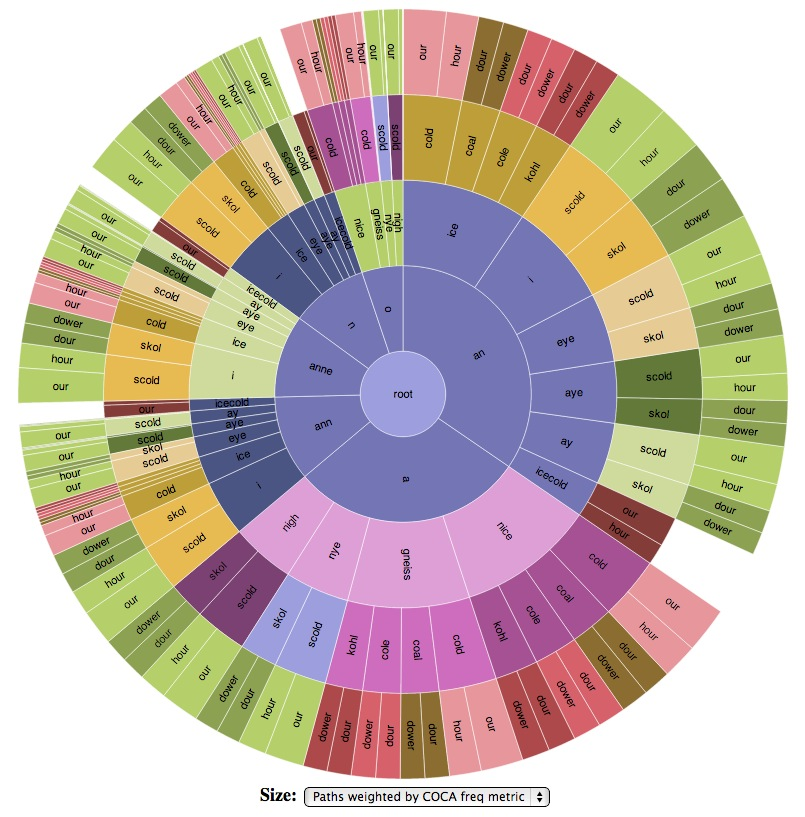
\includegraphics[width=\textwidth]{aNiceColdHour_COCA_FreqMetric.jpg}
\captionfonts
\caption[Sunburst diagram for ``an ice cold hour'' using COCA by-document freq metric]{Sunburst diagram for ``an ice cold hour'' using COCA by-document freq metric }
\label{fig:futureWork:COCAsunburst}
\end{figure}

\begin{figure}
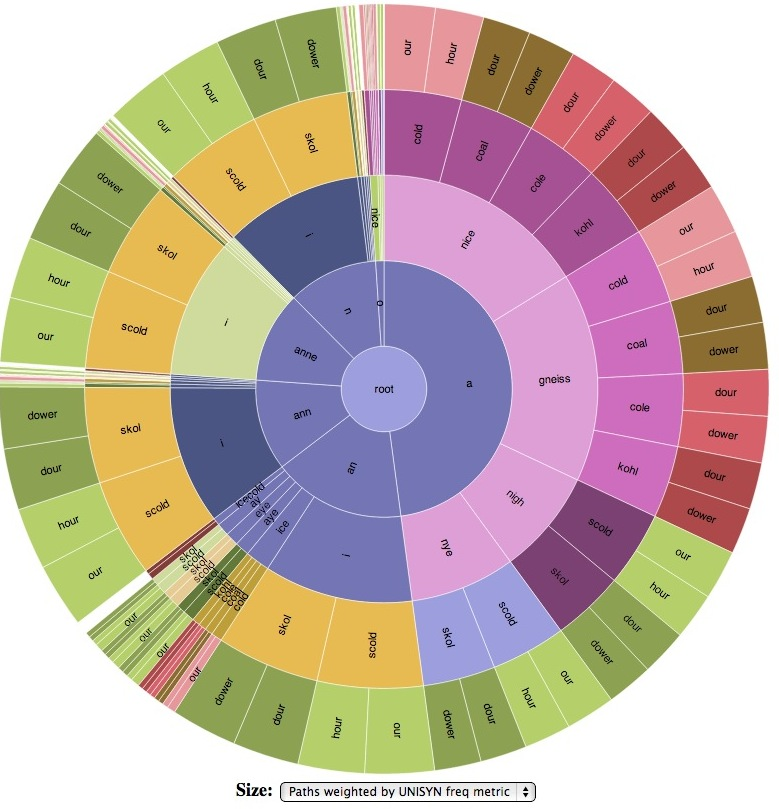
\includegraphics[width=\textwidth]{aNiceColdHour_UNISYN_FreqMetric.jpg}
\captionfonts
\caption[Sunburst diagram for ``an ice cold hour'' using UNISYN freq metric]{Sunburst diagram for ``an ice cold hour'' using UNISYN freq metric }
\label{fig:futureWork:UNISYNsunburst}
\end{figure}

%%%Insert here: statistics! Grab and adapt from 5.2.3 or something like that...


A statistical analysisof the observed dataset frequencies versus a COCA-derived frequency dataset, using a one-proportion z test, further proves that the COCA frequency values are a better match for the observed data than the UNISYN-derived frequencies.  Again using the top two observed transcriptions as our sample population, we take a look at the phrases \phraseOne and \phraseTwo.  The phrase \phraseOne has a calculated COCA freq metric of \cocaFreqForPhraseOne, and had \USATranscriptionsOfPhraseOne actual transcriptions observed among people living in the United States. The \phraseTwo has a calculated COCA freq metric of \cocaFreqForPhraseTwo, and had \USATranscriptionsOfPhraseTwo actual transcriptions observed among people living in the United States. Therefore, the expected population is \cocaCombinedFreq, and the observed population is \USACombinedTranscriptions.  

Given those population, the expected population proportion for \phraseOne would be \cocaFreqForPhraseOne  $\div$ \cocaCombinedFreq, or \expectedProportionOfPhraseOneOccurancesCOCA.  

In our user study, we found that \USATranscriptionsOfPhraseOne people transcribed \phraseOne, and \USATranscriptionsOfPhraseTwo people transcribed \phraseTwo, for a ratio of 0.65 to 1, where \phraseOne accounts for 39.56\% ( p = \observedProportionOfPhraseOneOccurances ) of the combined count. 

Given the observed population proportion of \observedProportionOfPhraseOneOccurances and the expected population proportion \expectedProportionOfPhraseOneOccurancesCOCA, we did a one-proportion z test with an $\alpha$ of \alphaSigFigs.  The z value returned was \COCAzVal, meaning that the observed population proportion was \COCAzVal standard deviations away from the expected population proportion.  When we used this z value to compute a p value, we were left with a pvalue of \pvalueCOCA, which is greater than our $\alpha$ of \alphaSigFigs. Therefore, there is approximately a 0.01\% chance that the observed data could match the COCA predictions, but it's still not incredibly likely. It's significantly more likely than the UNISYN predictions being correct, however.



\subsection{Higher-order frequency data}
\label{subsection:HigherOrderFrequencyData}

Right now, our program only takes into account the frequency of standalone words, without taking their context into consideration.  In the future, we'd like to integrate n-grams into our program. N-grams are a probabilistic model of predicting the next item that will follow in a sequence, based upon frequencies of how often those N items occur in sequence in a corpus of text\cite{ngramSiteFreeLists}.  A word-level 4-gram, for example, would be a series of four words. Here are some 4-gram phrases, along with counts of how often they occur, from the Google Ngram corpus:
\begin{quote}
serve as the informational 41 \\
serve as the infrastructure 500 \\
serve as the initial 5331\\
serve as the initiating 125\\
serve as the initiation 63\\
serve as the initiator 81\\
serve as the injector 56\\
serve as the inlet 41\\
serve as the inner 87\\
serve as the input 1323\\
\end{quote} \cite{allOurNgramsAreBelongToYou}

To give an example of what that might look like, we looked up historical n-gram occurence percentage of n-grams contained in oronyms of our main test phrase ``an ice cold hour''.  As seen in figure ~\ref{fig:futureWork:ThreeGram}, comparing the 3-grams ``a nice cold'' and ``an ice cold'' results in a fairly even split, though the latter phrase is slightly more likely to occur in modern-day settings. When we look at the 2-grams of that 3-gram, we see more interesting trends. In figure ~\ref{fig:futureWork:TwoGramAnice}, we see that ``a nice'' is consistently more frequently found in text than ``an ice'' is. However, when we compare the 2-grams ``ice cold'' and ``nice cold'', as we do in figure ~\ref{fig:futureWork:TwoGramIceCold}, we see that the phrase ``ice cold'' is leaps and bounds more likely to be encountered in everyday language.

\begin{figure}
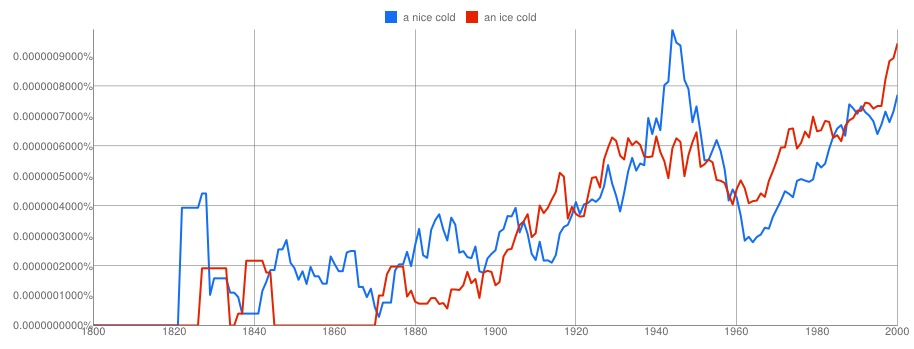
\includegraphics[width=\textwidth]{googleNgram_aNiceColdVSanIceCold.jpg}
\captionfonts
\caption[Historical N-gram data comparing the three-grams ``a nice cold'' and ``an ice cold'']{Historical N-gram data comparing the three-grams ``a nice cold'' and ``an ice cold''}
\label{fig:futureWork:ThreeGram}
\end{figure}


\begin{figure}
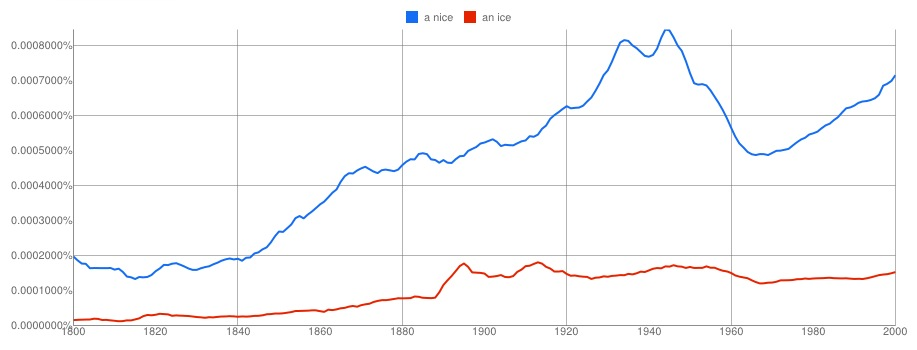
\includegraphics[width=\textwidth]{googleNgram_aNiceVSanIce.jpg}
\captionfonts
\caption[Historical N-gram data comparing the two-grams ``a nice'' and ``an ice'']{Historical N-gram data comparing the two-grams ``a nice'' and ``an ice''}
\label{fig:futureWork:TwoGramAnice}
\end{figure}

\begin{figure}
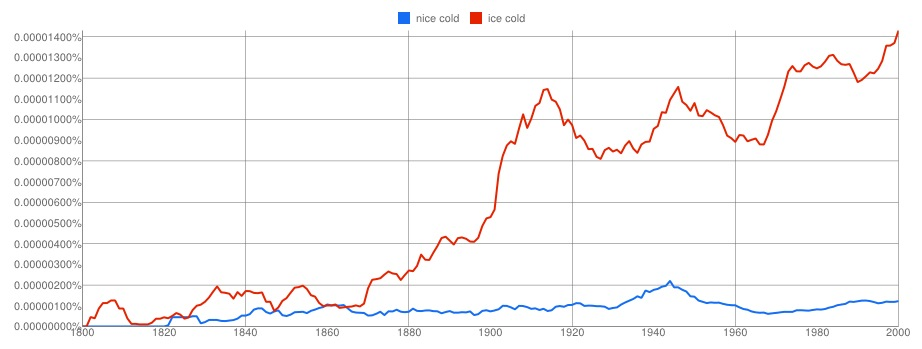
\includegraphics[width=\textwidth]{googleNgram_iceColdVSniceCold.jpg}
\captionfonts
\caption[Historical N-gram data comparing the two-grams ``nice cold'' and ``ice cold'']{Historical N-gram data comparing the two-grams ``nice cold'' and ``ice cold''}
\label{fig:futureWork:TwoGramIceCold}
\end{figure}


Though we are happy with our findings, we believe that we could create even better likelihood metrics with the integration of several different orders of n-grams, and would suggest this for future work.  However, if the final purpose of the oronyminator ends up being in the song lyric domain, everyday-usage syntactical predictability may not be particularly relevant, due to the differences in vocabulary and grammar found in song lyrics versus regular prose.


\section{Phoneme swapping}
\label{section:phonemeSwapping}

Often when speaking, humans substitute easier-to-say phones for more time-intensive phones.  One of the main ways that this substitution occurs is through voiced/voiceless pairs.  To “voice” a phone means to cause the vocal chords to vibrate.  “Voiced” phones are singable, whereas “voiceless” phones are not.  “Voiceless” phones are like a hiss, and simply direct streams of escaping air.  Most consonant phonemes are part of a voice/voiceless pair, such as `t' and `d' (The word ``pretty", when spoken quickly, often uses a `d' sound instead of a `t' sound, because the phoneme for `d' is easier to say). Phones are paired when the only differences between their pronuciation is the voicing, aka, when their manner of articulation (i.e. their manner of directing air during the sound), mouth end position, and mouth start position are the same (To view all phones in the SAMPA alphabet, along with enough information to determine whether they are pairs, see table ~\ref{sampaTable}). In our project, we came across an example of phoneme swapping in the ``cold''/``gold'' transcriptions, which we went over in figure ~\ref{fig:results:transcriptionCountPerRecordingANiceGoldHour} and section ~\ref{results:transcriptionCountPerRecording:a_nice_gold_hour}. For future work, we suggest looking into phoneme swap pairings, and integrating the findings into the existing algorithm. 


\section{Melody Matcher master project}
\label{melodyMatcherMasterProject}
MisheardMe Oronyminator is a part of the greater Melody Matcher suite. Melody Matcher is a semi-automated music composition support program. It analyzes English lyrics along with a melody, and alerts the composer of the locations in the song where the lyrics are not deterministically understandable. Basically, it's grammar- and spell-check for songs. 

\vspace{14pt}
Melody Matcher aims to replicate the human ability to identify lyrics in a song that are easily misheard. 
\vspace{14pt}

\subsection{Target Audience and Goals}
This program is to be used as a compositional aid by anyone who wants to write songs and make them sound good, technically. It should allow the song writer to focus on more subjective criteria of what makes a song ``good'', because it will make the structural rules of lyric composition immediately apparent.

Our hope for this project is that it will be useful to burgeoning songwriters, who have the creative spark to make wonderfully poetic lyrics, but lack the ``ear'' to match their lyrics successfully to music. It should be particularly helpful to songwriters who place a high emphasis on understandability of lyrics (such as parody song writers, or lyricists for musical theater).

Additionally, Melody Matcher will be useful for songwriters for whom English is a second language. While they may be a master lyricist in their native language, writing lyrics in English can be a particular challenge, since so much of lyric-writing is dependent upon knowing the cadence of the language you're writing lyrics in, and since English has no easily-discernible rules for emphasis placement in words.



While MisheardMe Oronyminator only takes into account phonetics and frequencies, Melody Matcher analyzes the intelligibility of song lyrics by investigating several additional root causes:


\begin{itemize} 
\item Lyric/Music emphasis mismatch, due to: 

    \begin{itemize} 
    \item Note intervals
    \item Phrase emphases
    \item Word emphases
    \end{itemize} 

\item Word ``cramming'', due to:

    \begin{itemize} 
    \item Syllable lengths that exceed that of note length
    \item Mouth movement delta time intervals
    \end{itemize} 

\item Word misidentification, due to:

    \begin{itemize} 
    \item Altered pronunciation of words
    \item Phone similarity

        \begin{itemize} 
        \item Voicing (voiced vs. voiceless)
        \item Beginning/end mouth positions
        \item Type (Plosive, Fricative, affricate, nasal, lateral, approximant, semivowel)
        \end{itemize} 
    
    \end{itemize} 
    \end{itemize} 

The fully-implemented Melody Matcher program will eventually take into account all of these causes of unintelligibility. 



\chapter{Conclusion}
\label{conclusion}

In this paper, we have demonstrated  MisheardMe Oronyminator, a computer program which takes in textual phrases in English, determines all oronyms for that phrase and then visualizes them using associated frequency information to indicate the likelihood of interpretation.
We have demonstrated all four major functional parts: our custom phonetic dictionary, our command-line oronym generator, our OpenGL oronym-parse-tree visualization generator, and our Protovis sunburst diagrams.  Our custom phonetic dictionary has some inconsistencies in word frenquency, due to the UNISYN source dictionary's frequency values not being generated from a well-sampled corpus. However, our program has no major structural flaws, and can be succesfully used for phrase with words with frequencies on the same order of magnitude. Our command-line oronym generator successfully generates all oronyms that are exact phonetic matches for an orthographic phrase.  The user studies that we did supported our generated phrases, if not our frequency metrics.  Our oronym visualizations had two goals: one, visually represent the likelihood of each oronym interpretation, visualized by scaling branches or arcs by phrase frequency values; and two, to exhibit orthographic phrases that may not have any exact oronyms, but have many dead-end, partial oronyms that could cause ambiguity. Our visualizations successfully accomplish both of those goals.




% ------------- End main chapters ----------------------

\clearpage

\pagebreak
\appendix

\include{appendices}
\addcontentsline{toc}{chapter}{Appendices}
\label{appendices}

%\appendix
\chapter{Implementation Details}
\label{appendix:table:implDetails}


\setlength\LTleft{-2in}
\begin{figure}
\begin{verbatim}
findAllPhoneSeqsForOrthoPhrase( orthoPhrase ) {
  allFullPhrasePhoneSeqs = empty list of list of phones
  orthoWords = split orthoPhrase on spaces
  
  origNumFullPhrases = 0
  for( orthoWord in orthoWords with index i ) {
    nextWordSampaPhoneSeqs = possible phone seqs following orthoWord
    
    if ( orthoWord is the first word in orthoPhrase ) {
      for( phoneSubSeq in nextWordSampaPhoneSeqs ) {
        append phoneSubSeq to allFullPhrasePhoneSeqs[i]
      }
    } else {
      origNumFullPhrases = allFullPhrasePhoneSeqs.size()
      if there’s more than one vector <phone> in nextWordSampaPhoneSeqs
        then we need to create duplicates of all existing allFullPhrasePhoneSeqs
    }
    
    for( m = 0 to allPhrasePhoneSeqs.size() ) {
      phraseToAppendIndex = m / origNumFullPhrases
      phoneSeqToAppend = nextWordSampaPhoneSeqs[phraseToAppendIndex]
      append phoneSeqToAppend to allFullPhrasePhoneSeqs[m]
    }
  }

  return allFullPhrasePhoneSeqs
}
\end{verbatim}
\captionfonts
\caption[Pseudocode for findAllPhoneSeqsForOrthoPhrase]{ Algorithm to get all phonetic sequences for an orthographic phrase. }
\label{fig:psuedoCode:findAllPhoneSeqsForOrthoPhrase}
\end{figure}
%\setlength\LTleft{2in}




\setlength\LTleft{-2in}
\begin{figure}
\begin{verbatim}
discoverOronymsForPhrase( origOrthoPhrase, includeDeadends ) {
   orthoMisheardAsPhrases = empty list
   allPhoneSeqsOfOrigPhrase = origOrthoPhrase.findAllPhoneSeqs()
   
   for( curPhoneSeqWithEmph in allPhoneSeqsOfOrigPhrase ) {
      // Remove emphasis marking for easier lookups
      curPhoneSeq = curPhoneSeqWithEmph.stripEmphasis()

      altOrthoPhrases = findOrthoStrsForPhoneSeq( curPhoneSeq )
      
      for( altOrthoPhrase in altOrthoPhrases ) {
         // Ensure it contains valid ortho text in all cases, and if
         // includeDeadends=false, contains no deadEndDelims so we only add
         // fully valid strings
         if ( ( includeDeadends == true &&
                altOrthoPhrase != deadEndDelim1 &&
                altOrthoPhrase != deadEndDelim2 ) ||
              ( altOrthoPhrase.contains( deadEndDelim1 ) == false &&
                altOrthoPhrase.contains( deadEndDelim2 ) == false ) ) {
            append altOrthoPhrase to orthoMisheardAsPhrases
         }
      }
   }
   
   orthoMisheardAsPhrases.removeDuplicates()

   return orthoMisheardAsPhrases
}
\end{verbatim}
\captionfonts
\caption[Pseudocode for discoverOronymsForPhrase]{ Algorithm to get all oronyms for an orthographic phrase. }
\label{fig:psuedoCode:discoverOronymsForPhrase}
\end{figure}
\setlength\LTleft{2in}

\begin{figure}
\begin{verbatim}
buildAndDrawFullTree( orthoPhrase ) {
   fullPhrases = orthoPhrase.discoverOronyms()
   (maxWordFreq, minWordFreq) = fullPhrases.getMaxAndMin()
   
   // Draw the tree's seed.
   glPushMatrix()
   {
      glTranslated(0.0, -1.0 * DEFAULT_BRANCH_LEN, 0.0)
      materials(GreenShiny)
      drawSphere(DEFAULT_RADIUS)
      materials(allMaterials.at( mat % allMaterials.size() ) )
      
      drawBranchesAtFork ( fullPhrases, DEFAULT_RADIUS )
   }
   glPopMatrix()
}
\end{verbatim}
\captionfonts
\caption[Code for buildAndDrawFullTree]{ Given an orthographic phrase, this function prepares to draw the tree }
\label{fig:psuedoCode:buildAndDrawFullTree}
\end{figure}


\begin{figure}
\begin{adjustwidth}{-1in}{}
\begin{verbatim}
drawBranchesAtFork( fullPhrases, lastRadius) {
   if( fullPhrases.size() == 0 ) {
      return
   }
   
   // Use a set to ensure no duplicates.
   firstWords = empty set
   
   for( phrase in fullPhrases ) {
      if( phrase.size() > 0 ) {
         firstWords.insert( phrase.firstWord() )
      }
   }
   
   // Calculate positioning variables for the spread of branches for firstWords.
   for ( curFirstWord in firstWords ) {
      firstWordFreq = curFirstWord.frequency()
      newAdditiveRadius = firstWordFreq.scaleToRadius()

      glPushMatrix()
      {
         // Translate and rotate into place
         if( curFirstWord == deadEndDelim1 || curFirstWord == deadEndDelim2 ) {
            // Draw a red sphere at the end of the last branch
         } else if ( curFirstWord == successDelim ) {
            // Draw a green sphere at the end of the last branch
         } else {
            // Draw a branch
            drawBranch( radiansToDegrees(tiltAngle), curXOffset, curYOffset,
                        newAdditiveRadius, lastRadius )
            
            // Find all phrases in fullPhrases that start with that firstWord
            tailsVect = fullPhrases.findAllWithPrefix(curFirstWord)
            
            // Change the colors for each branch level

            // Pass those phrases to drawBranchesAtFork
            drawBranchesAtFork( tailsVect, newAdditiveRadius, curXOffset, curYOffset )
            
            // Change the colors back to ensure consistency for each branch level
         }
      }
      glPopMatrix()
   }
}
\end{verbatim}
\end{adjustwidth}
\captionfonts
\caption[Code for drawBranchesAtFork]{ This is the function that facilitates the in-time drawing of the tree as we parse though our oronyms possibilities }
\label{fig:psuedoCode:drawBranchesAtFork}
\end{figure}


%\appendix
\chapter{Oronym Tables}
\label{appendix:table:oronymTable}

\setlength\LTleft{-1in}


\begin {longtable}{ cc|cccccccc }
\caption[All Oronyms for `A Nice Cold Hour' with frequency values]{All Oronyms for `A Nice Cold Hour' with frequency values}
\label{table:aNiceColdHourOronymWithFreqsTable}

\hline
phrase  &   total freq  &  word1  &  freq1  &  word2  &  freq2  &  word3  &  freq3  &  word4  &  freq4   \\ \hline
\endfirsthead

\multicolumn{10}{c}%
{{\bfseries \tablename\ \thetable{} -- continued from previous page}} \\
\hline
phrase  &   total freq  &  word1  &  freq1  &  word2  &  freq2  &  word3  &  freq3  &  word4  &  freq4   \\ \hline
\endhead

\hline \multicolumn{10}{|r|}{{Continued on next page}} \\ \hline
\endfoot

\hline \hline
\endlastfoot

 on i scold our   &  13185760  &   on   &  2774243  &   i   &  9937877  &   scold   &  217  &   our   &  473423   \\ \hline
 on i scold hour   &  12784150  &   on   &  2774243  &   i   &  9937877  &   scold   &  217  &   hour   &  71813   \\ \hline
 on i skol dour   &  12712244  &   on   &  2774243  &   i   &  9937877  &   skol   &  5  &   dour   &  119   \\ \hline
 on i skol dower   &  12712217  &   on   &  2774243  &   i   &  9937877  &   skol   &  5  &   dower   &  92   \\ \hline
 an i scold our   &  11205686  &   an   &  794169  &   i   &  9937877  &   scold   &  217  &   our   &  473423   \\ \hline
 an i scold hour   &  10804076  &   an   &  794169  &   i   &  9937877  &   scold   &  217  &   hour   &  71813   \\ \hline
 an i skol dour   &  10732170  &   an   &  794169  &   i   &  9937877  &   skol   &  5  &   dour   &  119   \\ \hline
 an i skol dower   &  10732143  &   an   &  794169  &   i   &  9937877  &   skol   &  5  &   dower   &  92   \\ \hline
 'n' i scold our   &  10411517  &   'n'   &  0  &   i   &  9937877  &   scold   &  217  &   our   &  473423   \\ \hline
 'n' i scold hour   &  10009907  &   'n'   &  0  &   i   &  9937877  &   scold   &  217  &   hour   &  71813   \\ \hline
 'n' i skol dour   &  9938001  &   'n'   &  0  &   i   &  9937877  &   skol   &  5  &   dour   &  119   \\ \hline
 'n' i skol dower   &  9937974  &   'n'   &  0  &   i   &  9937877  &   skol   &  5  &   dower   &  92   \\ \hline
 a nice cold our   &  8253272  &   a   &  7536297  &   nice   &  190708  &   cold   &  52844  &   our   &  473423   \\ \hline
 a niece cold our   &  8064257  &   a   &  7536297  &   niece   &  1693  &   cold   &  52844  &   our   &  473423   \\ \hline
 a gneiss cold our   &  8062585  &   a   &  7536297  &   gneiss   &  21  &   cold   &  52844  &   our   &  473423   \\ \hline
 a ne scold our   &  8017040  &   a   &  7536297  &   ne   &  7103  &   scold   &  217  &   our   &  473423   \\ \hline
 a knee scold our   &  8016076  &   a   &  7536297  &   knee   &  6139  &   scold   &  217  &   our   &  473423   \\ \hline
 a nigh scold our   &  8011331  &   a   &  7536297  &   nigh   &  1394  &   scold   &  217  &   our   &  473423   \\ \hline
 a nye scold our   &  8009974  &   a   &  7536297  &   nye   &  37  &   scold   &  217  &   our   &  473423   \\ \hline
 a nice cold hour   &  7851662  &   a   &  7536297  &   nice   &  190708  &   cold   &  52844  &   hour   &  71813   \\ \hline
 a nice coal dour   &  7747572  &   a   &  7536297  &   nice   &  190708  &   coal   &  20448  &   dour   &  119   \\ \hline
 a nice coal dower   &  7747545  &   a   &  7536297  &   nice   &  190708  &   coal   &  20448  &   dower   &  92   \\ \hline
 a nice cole dour   &  7729197  &   a   &  7536297  &   nice   &  190708  &   cole   &  2073  &   dour   &  119   \\ \hline
 a nice cole dower   &  7729170  &   a   &  7536297  &   nice   &  190708  &   cole   &  2073  &   dower   &  92   \\ \hline
 a nice kohl dour   &  7728036  &   a   &  7536297  &   nice   &  190708  &   kohl   &  912  &   dour   &  119   \\ \hline
 a nice kohl dower   &  7728009  &   a   &  7536297  &   nice   &  190708  &   kohl   &  912  &   dower   &  92   \\ \hline
 a niece cold hour   &  7662647  &   a   &  7536297  &   niece   &  1693  &   cold   &  52844  &   hour   &  71813   \\ \hline
 a gneiss cold hour   &  7660975  &   a   &  7536297  &   gneiss   &  21  &   cold   &  52844  &   hour   &  71813   \\ \hline
 a ne scold hour   &  7615430  &   a   &  7536297  &   ne   &  7103  &   scold   &  217  &   hour   &  71813   \\ \hline
 a knee scold hour   &  7614466  &   a   &  7536297  &   knee   &  6139  &   scold   &  217  &   hour   &  71813   \\ \hline
 a nigh scold hour   &  7609721  &   a   &  7536297  &   nigh   &  1394  &   scold   &  217  &   hour   &  71813   \\ \hline
 a nye scold hour   &  7608364  &   a   &  7536297  &   nye   &  37  &   scold   &  217  &   hour   &  71813   \\ \hline
 a niece coal dour   &  7558557  &   a   &  7536297  &   niece   &  1693  &   coal   &  20448  &   dour   &  119   \\ \hline
 a niece coal dower   &  7558530  &   a   &  7536297  &   niece   &  1693  &   coal   &  20448  &   dower   &  92   \\ \hline
 a gneiss coal dour   &  7556885  &   a   &  7536297  &   gneiss   &  21  &   coal   &  20448  &   dour   &  119   \\ \hline
 a gneiss coal dower   &  7556858  &   a   &  7536297  &   gneiss   &  21  &   coal   &  20448  &   dower   &  92   \\ \hline
 a ne skol dour   &  7543524  &   a   &  7536297  &   ne   &  7103  &   skol   &  5  &   dour   &  119   \\ \hline
 a ne skol dower   &  7543497  &   a   &  7536297  &   ne   &  7103  &   skol   &  5  &   dower   &  92   \\ \hline
 a knee skol dour   &  7542560  &   a   &  7536297  &   knee   &  6139  &   skol   &  5  &   dour   &  119   \\ \hline
 a knee skol dower   &  7542533  &   a   &  7536297  &   knee   &  6139  &   skol   &  5  &   dower   &  92   \\ \hline
 a niece cole dour   &  7540182  &   a   &  7536297  &   niece   &  1693  &   cole   &  2073  &   dour   &  119   \\ \hline
 a niece cole dower   &  7540155  &   a   &  7536297  &   niece   &  1693  &   cole   &  2073  &   dower   &  92   \\ \hline
 a niece kohl dour   &  7539021  &   a   &  7536297  &   niece   &  1693  &   kohl   &  912  &   dour   &  119   \\ \hline
 a niece kohl dower   &  7538994  &   a   &  7536297  &   niece   &  1693  &   kohl   &  912  &   dower   &  92   \\ \hline
 a gneiss cole dour   &  7538510  &   a   &  7536297  &   gneiss   &  21  &   cole   &  2073  &   dour   &  119   \\ \hline
 a gneiss cole dower   &  7538483  &   a   &  7536297  &   gneiss   &  21  &   cole   &  2073  &   dower   &  92   \\ \hline
 a nigh skol dour   &  7537815  &   a   &  7536297  &   nigh   &  1394  &   skol   &  5  &   dour   &  119   \\ \hline
 a nigh skol dower   &  7537788  &   a   &  7536297  &   nigh   &  1394  &   skol   &  5  &   dower   &  92   \\ \hline
 a gneiss kohl dour   &  7537349  &   a   &  7536297  &   gneiss   &  21  &   kohl   &  912  &   dour   &  119   \\ \hline
 a gneiss kohl dower   &  7537322  &   a   &  7536297  &   gneiss   &  21  &   kohl   &  912  &   dower   &  92   \\ \hline
 a nye skol dour   &  7536458  &   a   &  7536297  &   nye   &  37  &   skol   &  5  &   dour   &  119   \\ \hline
 a nye skol dower   &  7536431  &   a   &  7536297  &   nye   &  37  &   skol   &  5  &   dower   &  92   \\ \hline
 on aye scold our   &  3378386  &   on   &  2774243  &   aye   &  130503  &   scold   &  217  &   our   &  473423   \\ \hline
 on e scold our   &  3356846  &   on   &  2774243  &   e   &  108963  &   scold   &  217  &   our   &  473423   \\ \hline
 on ice cold our   &  3312712  &   on   &  2774243  &   ice   &  12202  &   cold   &  52844  &   our   &  473423   \\ \hline
 on eye scold our   &  3274633  &   on   &  2774243  &   eye   &  26750  &   scold   &  217  &   our   &  473423   \\ \hline
 on ay scold our   &  3254516  &   on   &  2774243  &   ay   &  6633  &   scold   &  217  &   our   &  473423   \\ \hline
 on ice-cold our   &  3247715  &   on   &  2774243  &   ice-cold   &  49  &   our   &  473423  &     &     \\ \hline
 on aye scold hour   &  2976776  &   on   &  2774243  &   aye   &  130503  &   scold   &  217  &   hour   &  71813   \\ \hline
 on e scold hour   &  2955236  &   on   &  2774243  &   e   &  108963  &   scold   &  217  &   hour   &  71813   \\ \hline
 on ice cold hour   &  2911102  &   on   &  2774243  &   ice   &  12202  &   cold   &  52844  &   hour   &  71813   \\ \hline
 on aye skol dour   &  2904870  &   on   &  2774243  &   aye   &  130503  &   skol   &  5  &   dour   &  119   \\ \hline
 on aye skol dower   &  2904843  &   on   &  2774243  &   aye   &  130503  &   skol   &  5  &   dower   &  92   \\ \hline
 on e skol dour   &  2883330  &   on   &  2774243  &   e   &  108963  &   skol   &  5  &   dour   &  119   \\ \hline
 on e skol dower   &  2883303  &   on   &  2774243  &   e   &  108963  &   skol   &  5  &   dower   &  92   \\ \hline
 on eye scold hour   &  2873023  &   on   &  2774243  &   eye   &  26750  &   scold   &  217  &   hour   &  71813   \\ \hline
 on ay scold hour   &  2852906  &   on   &  2774243  &   ay   &  6633  &   scold   &  217  &   hour   &  71813   \\ \hline
 on ice-cold hour   &  2846105  &   on   &  2774243  &   ice-cold   &  49  &   hour   &  71813  &     &     \\ \hline
 on ice coal dour   &  2807012  &   on   &  2774243  &   ice   &  12202  &   coal   &  20448  &   dour   &  119   \\ \hline
 on ice coal dower   &  2806985  &   on   &  2774243  &   ice   &  12202  &   coal   &  20448  &   dower   &  92   \\ \hline
 on eye skol dour   &  2801117  &   on   &  2774243  &   eye   &  26750  &   skol   &  5  &   dour   &  119   \\ \hline
 on eye skol dower   &  2801090  &   on   &  2774243  &   eye   &  26750  &   skol   &  5  &   dower   &  92   \\ \hline
 on ice cole dour   &  2788637  &   on   &  2774243  &   ice   &  12202  &   cole   &  2073  &   dour   &  119   \\ \hline
 on ice cole dower   &  2788610  &   on   &  2774243  &   ice   &  12202  &   cole   &  2073  &   dower   &  92   \\ \hline
 on ice kohl dour   &  2787476  &   on   &  2774243  &   ice   &  12202  &   kohl   &  912  &   dour   &  119   \\ \hline
 on ice kohl dower   &  2787449  &   on   &  2774243  &   ice   &  12202  &   kohl   &  912  &   dower   &  92   \\ \hline
 on ay skol dour   &  2781000  &   on   &  2774243  &   ay   &  6633  &   skol   &  5  &   dour   &  119   \\ \hline
 on ay skol dower   &  2780973  &   on   &  2774243  &   ay   &  6633  &   skol   &  5  &   dower   &  92   \\ \hline
 an aye scold our   &  1398312  &   an   &  794169  &   aye   &  130503  &   scold   &  217  &   our   &  473423   \\ \hline
 an e scold our   &  1376772  &   an   &  794169  &   e   &  108963  &   scold   &  217  &   our   &  473423   \\ \hline
 an ice cold our   &  1332638  &   an   &  794169  &   ice   &  12202  &   cold   &  52844  &   our   &  473423   \\ \hline
 an eye scold our   &  1294559  &   an   &  794169  &   eye   &  26750  &   scold   &  217  &   our   &  473423   \\ \hline
 an ay scold our   &  1274442  &   an   &  794169  &   ay   &  6633  &   scold   &  217  &   our   &  473423   \\ \hline
 an ice-cold our   &  1267641  &   an   &  794169  &   ice-cold   &  49  &   our   &  473423  &     &     \\ \hline
 an aye scold hour   &  996702  &   an   &  794169  &   aye   &  130503  &   scold   &  217  &   hour   &  71813   \\ \hline
 an e scold hour   &  975162  &   an   &  794169  &   e   &  108963  &   scold   &  217  &   hour   &  71813   \\ \hline
 ah nice cold our   &  946271  &   ah   &  229296  &   nice   &  190708  &   cold   &  52844  &   our   &  473423   \\ \hline
 an ice cold hour   &  931028  &   an   &  794169  &   ice   &  12202  &   cold   &  52844  &   hour   &  71813   \\ \hline
 an aye skol dour   &  924796  &   an   &  794169  &   aye   &  130503  &   skol   &  5  &   dour   &  119   \\ \hline
 an aye skol dower   &  924769  &   an   &  794169  &   aye   &  130503  &   skol   &  5  &   dower   &  92   \\ \hline
 an e skol dour   &  903256  &   an   &  794169  &   e   &  108963  &   skol   &  5  &   dour   &  119   \\ \hline
 an e skol dower   &  903229  &   an   &  794169  &   e   &  108963  &   skol   &  5  &   dower   &  92   \\ \hline
 an eye scold hour   &  892949  &   an   &  794169  &   eye   &  26750  &   scold   &  217  &   hour   &  71813   \\ \hline
 an ay scold hour   &  872832  &   an   &  794169  &   ay   &  6633  &   scold   &  217  &   hour   &  71813   \\ \hline
 an ice-cold hour   &  866031  &   an   &  794169  &   ice-cold   &  49  &   hour   &  71813  &     &     \\ \hline
 an ice coal dour   &  826938  &   an   &  794169  &   ice   &  12202  &   coal   &  20448  &   dour   &  119   \\ \hline
 an ice coal dower   &  826911  &   an   &  794169  &   ice   &  12202  &   coal   &  20448  &   dower   &  92   \\ \hline
 an eye skol dour   &  821043  &   an   &  794169  &   eye   &  26750  &   skol   &  5  &   dour   &  119   \\ \hline
 an eye skol dower   &  821016  &   an   &  794169  &   eye   &  26750  &   skol   &  5  &   dower   &  92   \\ \hline
 an ice cole dour   &  808563  &   an   &  794169  &   ice   &  12202  &   cole   &  2073  &   dour   &  119   \\ \hline
 an ice cole dower   &  808536  &   an   &  794169  &   ice   &  12202  &   cole   &  2073  &   dower   &  92   \\ \hline
 an ice kohl dour   &  807402  &   an   &  794169  &   ice   &  12202  &   kohl   &  912  &   dour   &  119   \\ \hline
 an ice kohl dower   &  807375  &   an   &  794169  &   ice   &  12202  &   kohl   &  912  &   dower   &  92   \\ \hline
 an ay skol dour   &  800926  &   an   &  794169  &   ay   &  6633  &   skol   &  5  &   dour   &  119   \\ \hline
 an ay skol dower   &  800899  &   an   &  794169  &   ay   &  6633  &   skol   &  5  &   dower   &  92   \\ \hline
 eh nice cold our   &  783938  &   eh   &  66963  &   nice   &  190708  &   cold   &  52844  &   our   &  473423   \\ \hline
 ah niece cold our   &  757256  &   ah   &  229296  &   niece   &  1693  &   cold   &  52844  &   our   &  473423   \\ \hline
 ah gneiss cold our   &  755584  &   ah   &  229296  &   gneiss   &  21  &   cold   &  52844  &   our   &  473423   \\ \hline
 et nice cold our   &  723706  &   et   &  6731  &   nice   &  190708  &   cold   &  52844  &   our   &  473423   \\ \hline
 o' nice cold our   &  717438  &   o'   &  463  &   nice   &  190708  &   cold   &  52844  &   our   &  473423   \\ \hline
 ah ne scold our   &  710039  &   ah   &  229296  &   ne   &  7103  &   scold   &  217  &   our   &  473423   \\ \hline
 ah knee scold our   &  709075  &   ah   &  229296  &   knee   &  6139  &   scold   &  217  &   our   &  473423   \\ \hline
 ah nigh scold our   &  704330  &   ah   &  229296  &   nigh   &  1394  &   scold   &  217  &   our   &  473423   \\ \hline
 ah nye scold our   &  702973  &   ah   &  229296  &   nye   &  37  &   scold   &  217  &   our   &  473423   \\ \hline
 'n' aye scold our   &  604143  &   'n'   &  0  &   aye   &  130503  &   scold   &  217  &   our   &  473423   \\ \hline
 eh niece cold our   &  594923  &   eh   &  66963  &   niece   &  1693  &   cold   &  52844  &   our   &  473423   \\ \hline
 eh gneiss cold our   &  593251  &   eh   &  66963  &   gneiss   &  21  &   cold   &  52844  &   our   &  473423   \\ \hline
 'n' e scold our   &  582603  &   'n'   &  0  &   e   &  108963  &   scold   &  217  &   our   &  473423   \\ \hline
 eh ne scold our   &  547706  &   eh   &  66963  &   ne   &  7103  &   scold   &  217  &   our   &  473423   \\ \hline
 eh knee scold our   &  546742  &   eh   &  66963  &   knee   &  6139  &   scold   &  217  &   our   &  473423   \\ \hline
 ah nice cold hour   &  544661  &   ah   &  229296  &   nice   &  190708  &   cold   &  52844  &   hour   &  71813   \\ \hline
 eh nigh scold our   &  541997  &   eh   &  66963  &   nigh   &  1394  &   scold   &  217  &   our   &  473423   \\ \hline
 eh nye scold our   &  540640  &   eh   &  66963  &   nye   &  37  &   scold   &  217  &   our   &  473423   \\ \hline
 'n' ice cold our   &  538469  &   'n'   &  0  &   ice   &  12202  &   cold   &  52844  &   our   &  473423   \\ \hline
 et niece cold our   &  534691  &   et   &  6731  &   niece   &  1693  &   cold   &  52844  &   our   &  473423   \\ \hline
 et gneiss cold our   &  533019  &   et   &  6731  &   gneiss   &  21  &   cold   &  52844  &   our   &  473423   \\ \hline
 o' niece cold our   &  528423  &   o'   &  463  &   niece   &  1693  &   cold   &  52844  &   our   &  473423   \\ \hline
 o' gneiss cold our   &  526751  &   o'   &  463  &   gneiss   &  21  &   cold   &  52844  &   our   &  473423   \\ \hline
 'n' eye scold our   &  500390  &   'n'   &  0  &   eye   &  26750  &   scold   &  217  &   our   &  473423   \\ \hline
 et ne scold our   &  487474  &   et   &  6731  &   ne   &  7103  &   scold   &  217  &   our   &  473423   \\ \hline
 et knee scold our   &  486510  &   et   &  6731  &   knee   &  6139  &   scold   &  217  &   our   &  473423   \\ \hline
 et nigh scold our   &  481765  &   et   &  6731  &   nigh   &  1394  &   scold   &  217  &   our   &  473423   \\ \hline
 o' ne scold our   &  481206  &   o'   &  463  &   ne   &  7103  &   scold   &  217  &   our   &  473423   \\ \hline
 et nye scold our   &  480408  &   et   &  6731  &   nye   &  37  &   scold   &  217  &   our   &  473423   \\ \hline
 'n' ay scold our   &  480273  &   'n'   &  0  &   ay   &  6633  &   scold   &  217  &   our   &  473423   \\ \hline
 o' knee scold our   &  480242  &   o'   &  463  &   knee   &  6139  &   scold   &  217  &   our   &  473423   \\ \hline
 o' nigh scold our   &  475497  &   o'   &  463  &   nigh   &  1394  &   scold   &  217  &   our   &  473423   \\ \hline
 o' nye scold our   &  474140  &   o'   &  463  &   nye   &  37  &   scold   &  217  &   our   &  473423   \\ \hline
 'n' ice-cold our   &  473472  &   'n'   &  0  &   ice-cold   &  49  &   our   &  473423  &     &     \\ \hline
 ah nice coal dour   &  440571  &   ah   &  229296  &   nice   &  190708  &   coal   &  20448  &   dour   &  119   \\ \hline
 ah nice coal dower   &  440544  &   ah   &  229296  &   nice   &  190708  &   coal   &  20448  &   dower   &  92   \\ \hline
 ah nice cole dour   &  422196  &   ah   &  229296  &   nice   &  190708  &   cole   &  2073  &   dour   &  119   \\ \hline
 ah nice cole dower   &  422169  &   ah   &  229296  &   nice   &  190708  &   cole   &  2073  &   dower   &  92   \\ \hline
 ah nice kohl dour   &  421035  &   ah   &  229296  &   nice   &  190708  &   kohl   &  912  &   dour   &  119   \\ \hline
 ah nice kohl dower   &  421008  &   ah   &  229296  &   nice   &  190708  &   kohl   &  912  &   dower   &  92   \\ \hline
 eh nice cold hour   &  382328  &   eh   &  66963  &   nice   &  190708  &   cold   &  52844  &   hour   &  71813   \\ \hline
 ah niece cold hour   &  355646  &   ah   &  229296  &   niece   &  1693  &   cold   &  52844  &   hour   &  71813   \\ \hline
 ah gneiss cold hour   &  353974  &   ah   &  229296  &   gneiss   &  21  &   cold   &  52844  &   hour   &  71813   \\ \hline
 et nice cold hour   &  322096  &   et   &  6731  &   nice   &  190708  &   cold   &  52844  &   hour   &  71813   \\ \hline
 o' nice cold hour   &  315828  &   o'   &  463  &   nice   &  190708  &   cold   &  52844  &   hour   &  71813   \\ \hline
 ah ne scold hour   &  308429  &   ah   &  229296  &   ne   &  7103  &   scold   &  217  &   hour   &  71813   \\ \hline
 ah knee scold hour   &  307465  &   ah   &  229296  &   knee   &  6139  &   scold   &  217  &   hour   &  71813   \\ \hline
 ah nigh scold hour   &  302720  &   ah   &  229296  &   nigh   &  1394  &   scold   &  217  &   hour   &  71813   \\ \hline
 ah nye scold hour   &  301363  &   ah   &  229296  &   nye   &  37  &   scold   &  217  &   hour   &  71813   \\ \hline
 eh nice coal dour   &  278238  &   eh   &  66963  &   nice   &  190708  &   coal   &  20448  &   dour   &  119   \\ \hline
 eh nice coal dower   &  278211  &   eh   &  66963  &   nice   &  190708  &   coal   &  20448  &   dower   &  92   \\ \hline
 eh nice cole dour   &  259863  &   eh   &  66963  &   nice   &  190708  &   cole   &  2073  &   dour   &  119   \\ \hline
 eh nice cole dower   &  259836  &   eh   &  66963  &   nice   &  190708  &   cole   &  2073  &   dower   &  92   \\ \hline
 eh nice kohl dour   &  258702  &   eh   &  66963  &   nice   &  190708  &   kohl   &  912  &   dour   &  119   \\ \hline
 eh nice kohl dower   &  258675  &   eh   &  66963  &   nice   &  190708  &   kohl   &  912  &   dower   &  92   \\ \hline
 ah niece coal dour   &  251556  &   ah   &  229296  &   niece   &  1693  &   coal   &  20448  &   dour   &  119   \\ \hline
 ah niece coal dower   &  251529  &   ah   &  229296  &   niece   &  1693  &   coal   &  20448  &   dower   &  92   \\ \hline
 ah gneiss coal dour   &  249884  &   ah   &  229296  &   gneiss   &  21  &   coal   &  20448  &   dour   &  119   \\ \hline
 ah gneiss coal dower   &  249857  &   ah   &  229296  &   gneiss   &  21  &   coal   &  20448  &   dower   &  92   \\ \hline
 ah ne skol dour   &  236523  &   ah   &  229296  &   ne   &  7103  &   skol   &  5  &   dour   &  119   \\ \hline
 ah ne skol dower   &  236496  &   ah   &  229296  &   ne   &  7103  &   skol   &  5  &   dower   &  92   \\ \hline
 ah knee skol dour   &  235559  &   ah   &  229296  &   knee   &  6139  &   skol   &  5  &   dour   &  119   \\ \hline
 ah knee skol dower   &  235532  &   ah   &  229296  &   knee   &  6139  &   skol   &  5  &   dower   &  92   \\ \hline
 ah niece cole dour   &  233181  &   ah   &  229296  &   niece   &  1693  &   cole   &  2073  &   dour   &  119   \\ \hline
 ah niece cole dower   &  233154  &   ah   &  229296  &   niece   &  1693  &   cole   &  2073  &   dower   &  92   \\ \hline
 ah niece kohl dour   &  232020  &   ah   &  229296  &   niece   &  1693  &   kohl   &  912  &   dour   &  119   \\ \hline
 ah niece kohl dower   &  231993  &   ah   &  229296  &   niece   &  1693  &   kohl   &  912  &   dower   &  92   \\ \hline
 ah gneiss cole dour   &  231509  &   ah   &  229296  &   gneiss   &  21  &   cole   &  2073  &   dour   &  119   \\ \hline
 ah gneiss cole dower   &  231482  &   ah   &  229296  &   gneiss   &  21  &   cole   &  2073  &   dower   &  92   \\ \hline
 ah nigh skol dour   &  230814  &   ah   &  229296  &   nigh   &  1394  &   skol   &  5  &   dour   &  119   \\ \hline
 ah nigh skol dower   &  230787  &   ah   &  229296  &   nigh   &  1394  &   skol   &  5  &   dower   &  92   \\ \hline
 ah gneiss kohl dour   &  230348  &   ah   &  229296  &   gneiss   &  21  &   kohl   &  912  &   dour   &  119   \\ \hline
 ah gneiss kohl dower   &  230321  &   ah   &  229296  &   gneiss   &  21  &   kohl   &  912  &   dower   &  92   \\ \hline
 ah nye skol dour   &  229457  &   ah   &  229296  &   nye   &  37  &   skol   &  5  &   dour   &  119   \\ \hline
 ah nye skol dower   &  229430  &   ah   &  229296  &   nye   &  37  &   skol   &  5  &   dower   &  92   \\ \hline
 et nice coal dour   &  218006  &   et   &  6731  &   nice   &  190708  &   coal   &  20448  &   dour   &  119   \\ \hline
 et nice coal dower   &  217979  &   et   &  6731  &   nice   &  190708  &   coal   &  20448  &   dower   &  92   \\ \hline
 o' nice coal dour   &  211738  &   o'   &  463  &   nice   &  190708  &   coal   &  20448  &   dour   &  119   \\ \hline
 o' nice coal dower   &  211711  &   o'   &  463  &   nice   &  190708  &   coal   &  20448  &   dower   &  92   \\ \hline
 'n' aye scold hour   &  202533  &   'n'   &  0  &   aye   &  130503  &   scold   &  217  &   hour   &  71813   \\ \hline
 et nice cole dour   &  199631  &   et   &  6731  &   nice   &  190708  &   cole   &  2073  &   dour   &  119   \\ \hline
 et nice cole dower   &  199604  &   et   &  6731  &   nice   &  190708  &   cole   &  2073  &   dower   &  92   \\ \hline
 et nice kohl dour   &  198470  &   et   &  6731  &   nice   &  190708  &   kohl   &  912  &   dour   &  119   \\ \hline
 et nice kohl dower   &  198443  &   et   &  6731  &   nice   &  190708  &   kohl   &  912  &   dower   &  92   \\ \hline
 o' nice cole dour   &  193363  &   o'   &  463  &   nice   &  190708  &   cole   &  2073  &   dour   &  119   \\ \hline
 o' nice cole dower   &  193336  &   o'   &  463  &   nice   &  190708  &   cole   &  2073  &   dower   &  92   \\ \hline
 eh niece cold hour   &  193313  &   eh   &  66963  &   niece   &  1693  &   cold   &  52844  &   hour   &  71813   \\ \hline
 o' nice kohl dour   &  192202  &   o'   &  463  &   nice   &  190708  &   kohl   &  912  &   dour   &  119   \\ \hline
 o' nice kohl dower   &  192175  &   o'   &  463  &   nice   &  190708  &   kohl   &  912  &   dower   &  92   \\ \hline
 eh gneiss cold hour   &  191641  &   eh   &  66963  &   gneiss   &  21  &   cold   &  52844  &   hour   &  71813   \\ \hline
 'n' e scold hour   &  180993  &   'n'   &  0  &   e   &  108963  &   scold   &  217  &   hour   &  71813   \\ \hline
 eh ne scold hour   &  146096  &   eh   &  66963  &   ne   &  7103  &   scold   &  217  &   hour   &  71813   \\ \hline
 eh knee scold hour   &  145132  &   eh   &  66963  &   knee   &  6139  &   scold   &  217  &   hour   &  71813   \\ \hline
 eh nigh scold hour   &  140387  &   eh   &  66963  &   nigh   &  1394  &   scold   &  217  &   hour   &  71813   \\ \hline
 eh nye scold hour   &  139030  &   eh   &  66963  &   nye   &  37  &   scold   &  217  &   hour   &  71813   \\ \hline
 'n' ice cold hour   &  136859  &   'n'   &  0  &   ice   &  12202  &   cold   &  52844  &   hour   &  71813   \\ \hline
 et niece cold hour   &  133081  &   et   &  6731  &   niece   &  1693  &   cold   &  52844  &   hour   &  71813   \\ \hline
 et gneiss cold hour   &  131409  &   et   &  6731  &   gneiss   &  21  &   cold   &  52844  &   hour   &  71813   \\ \hline
 'n' aye skol dour   &  130627  &   'n'   &  0  &   aye   &  130503  &   skol   &  5  &   dour   &  119   \\ \hline
 'n' aye skol dower   &  130600  &   'n'   &  0  &   aye   &  130503  &   skol   &  5  &   dower   &  92   \\ \hline
 o' niece cold hour   &  126813  &   o'   &  463  &   niece   &  1693  &   cold   &  52844  &   hour   &  71813   \\ \hline
 o' gneiss cold hour   &  125141  &   o'   &  463  &   gneiss   &  21  &   cold   &  52844  &   hour   &  71813   \\ \hline
 'n' e skol dour   &  109087  &   'n'   &  0  &   e   &  108963  &   skol   &  5  &   dour   &  119   \\ \hline
 'n' e skol dower   &  109060  &   'n'   &  0  &   e   &  108963  &   skol   &  5  &   dower   &  92   \\ \hline
 'n' eye scold hour   &  98780  &   'n'   &  0  &   eye   &  26750  &   scold   &  217  &   hour   &  71813   \\ \hline
 eh niece coal dour   &  89223  &   eh   &  66963  &   niece   &  1693  &   coal   &  20448  &   dour   &  119   \\ \hline
 eh niece coal dower   &  89196  &   eh   &  66963  &   niece   &  1693  &   coal   &  20448  &   dower   &  92   \\ \hline
 eh gneiss coal dour   &  87551  &   eh   &  66963  &   gneiss   &  21  &   coal   &  20448  &   dour   &  119   \\ \hline
 eh gneiss coal dower   &  87524  &   eh   &  66963  &   gneiss   &  21  &   coal   &  20448  &   dower   &  92   \\ \hline
 et ne scold hour   &  85864  &   et   &  6731  &   ne   &  7103  &   scold   &  217  &   hour   &  71813   \\ \hline
 et knee scold hour   &  84900  &   et   &  6731  &   knee   &  6139  &   scold   &  217  &   hour   &  71813   \\ \hline
 et nigh scold hour   &  80155  &   et   &  6731  &   nigh   &  1394  &   scold   &  217  &   hour   &  71813   \\ \hline
 o' ne scold hour   &  79596  &   o'   &  463  &   ne   &  7103  &   scold   &  217  &   hour   &  71813   \\ \hline
 et nye scold hour   &  78798  &   et   &  6731  &   nye   &  37  &   scold   &  217  &   hour   &  71813   \\ \hline
 'n' ay scold hour   &  78663  &   'n'   &  0  &   ay   &  6633  &   scold   &  217  &   hour   &  71813   \\ \hline
 o' knee scold hour   &  78632  &   o'   &  463  &   knee   &  6139  &   scold   &  217  &   hour   &  71813   \\ \hline
 eh ne skol dour   &  74190  &   eh   &  66963  &   ne   &  7103  &   skol   &  5  &   dour   &  119   \\ \hline
 eh ne skol dower   &  74163  &   eh   &  66963  &   ne   &  7103  &   skol   &  5  &   dower   &  92   \\ \hline
 o' nigh scold hour   &  73887  &   o'   &  463  &   nigh   &  1394  &   scold   &  217  &   hour   &  71813   \\ \hline
 eh knee skol dour   &  73226  &   eh   &  66963  &   knee   &  6139  &   skol   &  5  &   dour   &  119   \\ \hline
 eh knee skol dower   &  73199  &   eh   &  66963  &   knee   &  6139  &   skol   &  5  &   dower   &  92   \\ \hline
 o' nye scold hour   &  72530  &   o'   &  463  &   nye   &  37  &   scold   &  217  &   hour   &  71813   \\ \hline
 'n' ice-cold hour   &  71862  &   'n'   &  0  &   ice-cold   &  49  &   hour   &  71813  &     &     \\ \hline
 eh niece cole dour   &  70848  &   eh   &  66963  &   niece   &  1693  &   cole   &  2073  &   dour   &  119   \\ \hline
 eh niece cole dower   &  70821  &   eh   &  66963  &   niece   &  1693  &   cole   &  2073  &   dower   &  92   \\ \hline
 eh niece kohl dour   &  69687  &   eh   &  66963  &   niece   &  1693  &   kohl   &  912  &   dour   &  119   \\ \hline
 eh niece kohl dower   &  69660  &   eh   &  66963  &   niece   &  1693  &   kohl   &  912  &   dower   &  92   \\ \hline
 eh gneiss cole dour   &  69176  &   eh   &  66963  &   gneiss   &  21  &   cole   &  2073  &   dour   &  119   \\ \hline
 eh gneiss cole dower   &  69149  &   eh   &  66963  &   gneiss   &  21  &   cole   &  2073  &   dower   &  92   \\ \hline
 eh nigh skol dour   &  68481  &   eh   &  66963  &   nigh   &  1394  &   skol   &  5  &   dour   &  119   \\ \hline
 eh nigh skol dower   &  68454  &   eh   &  66963  &   nigh   &  1394  &   skol   &  5  &   dower   &  92   \\ \hline
 eh gneiss kohl dour   &  68015  &   eh   &  66963  &   gneiss   &  21  &   kohl   &  912  &   dour   &  119   \\ \hline
 eh gneiss kohl dower   &  67988  &   eh   &  66963  &   gneiss   &  21  &   kohl   &  912  &   dower   &  92   \\ \hline
 eh nye skol dour   &  67124  &   eh   &  66963  &   nye   &  37  &   skol   &  5  &   dour   &  119   \\ \hline
 eh nye skol dower   &  67097  &   eh   &  66963  &   nye   &  37  &   skol   &  5  &   dower   &  92   \\ \hline
 'n' ice coal dour   &  32769  &   'n'   &  0  &   ice   &  12202  &   coal   &  20448  &   dour   &  119   \\ \hline
 'n' ice coal dower   &  32742  &   'n'   &  0  &   ice   &  12202  &   coal   &  20448  &   dower   &  92   \\ \hline
 et niece coal dour   &  28991  &   et   &  6731  &   niece   &  1693  &   coal   &  20448  &   dour   &  119   \\ \hline
 et niece coal dower   &  28964  &   et   &  6731  &   niece   &  1693  &   coal   &  20448  &   dower   &  92   \\ \hline
 et gneiss coal dour   &  27319  &   et   &  6731  &   gneiss   &  21  &   coal   &  20448  &   dour   &  119   \\ \hline
 et gneiss coal dower   &  27292  &   et   &  6731  &   gneiss   &  21  &   coal   &  20448  &   dower   &  92   \\ \hline
 'n' eye skol dour   &  26874  &   'n'   &  0  &   eye   &  26750  &   skol   &  5  &   dour   &  119   \\ \hline
 'n' eye skol dower   &  26847  &   'n'   &  0  &   eye   &  26750  &   skol   &  5  &   dower   &  92   \\ \hline
 o' niece coal dour   &  22723  &   o'   &  463  &   niece   &  1693  &   coal   &  20448  &   dour   &  119   \\ \hline
 o' niece coal dower   &  22696  &   o'   &  463  &   niece   &  1693  &   coal   &  20448  &   dower   &  92   \\ \hline
 o' gneiss coal dour   &  21051  &   o'   &  463  &   gneiss   &  21  &   coal   &  20448  &   dour   &  119   \\ \hline
 o' gneiss coal dower   &  21024  &   o'   &  463  &   gneiss   &  21  &   coal   &  20448  &   dower   &  92   \\ \hline
 'n' ice cole dour   &  14394  &   'n'   &  0  &   ice   &  12202  &   cole   &  2073  &   dour   &  119   \\ \hline
 'n' ice cole dower   &  14367  &   'n'   &  0  &   ice   &  12202  &   cole   &  2073  &   dower   &  92   \\ \hline
 et ne skol dour   &  13958  &   et   &  6731  &   ne   &  7103  &   skol   &  5  &   dour   &  119   \\ \hline
 et ne skol dower   &  13931  &   et   &  6731  &   ne   &  7103  &   skol   &  5  &   dower   &  92   \\ \hline
 'n' ice kohl dour   &  13233  &   'n'   &  0  &   ice   &  12202  &   kohl   &  912  &   dour   &  119   \\ \hline
 'n' ice kohl dower   &  13206  &   'n'   &  0  &   ice   &  12202  &   kohl   &  912  &   dower   &  92   \\ \hline
 et knee skol dour   &  12994  &   et   &  6731  &   knee   &  6139  &   skol   &  5  &   dour   &  119   \\ \hline
 et knee skol dower   &  12967  &   et   &  6731  &   knee   &  6139  &   skol   &  5  &   dower   &  92   \\ \hline
 et niece cole dour   &  10616  &   et   &  6731  &   niece   &  1693  &   cole   &  2073  &   dour   &  119   \\ \hline
 et niece cole dower   &  10589  &   et   &  6731  &   niece   &  1693  &   cole   &  2073  &   dower   &  92   \\ \hline
 et niece kohl dour   &  9455  &   et   &  6731  &   niece   &  1693  &   kohl   &  912  &   dour   &  119   \\ \hline
 et niece kohl dower   &  9428  &   et   &  6731  &   niece   &  1693  &   kohl   &  912  &   dower   &  92   \\ \hline
 et gneiss cole dour   &  8944  &   et   &  6731  &   gneiss   &  21  &   cole   &  2073  &   dour   &  119   \\ \hline
 et gneiss cole dower   &  8917  &   et   &  6731  &   gneiss   &  21  &   cole   &  2073  &   dower   &  92   \\ \hline
 et nigh skol dour   &  8249  &   et   &  6731  &   nigh   &  1394  &   skol   &  5  &   dour   &  119   \\ \hline
 et nigh skol dower   &  8222  &   et   &  6731  &   nigh   &  1394  &   skol   &  5  &   dower   &  92   \\ \hline
 et gneiss kohl dour   &  7783  &   et   &  6731  &   gneiss   &  21  &   kohl   &  912  &   dour   &  119   \\ \hline
 et gneiss kohl dower   &  7756  &   et   &  6731  &   gneiss   &  21  &   kohl   &  912  &   dower   &  92   \\ \hline
 o' ne skol dour   &  7690  &   o'   &  463  &   ne   &  7103  &   skol   &  5  &   dour   &  119   \\ \hline
 o' ne skol dower   &  7663  &   o'   &  463  &   ne   &  7103  &   skol   &  5  &   dower   &  92   \\ \hline
 et nye skol dour   &  6892  &   et   &  6731  &   nye   &  37  &   skol   &  5  &   dour   &  119   \\ \hline
 et nye skol dower   &  6865  &   et   &  6731  &   nye   &  37  &   skol   &  5  &   dower   &  92   \\ \hline
 'n' ay skol dour   &  6757  &   'n'   &  0  &   ay   &  6633  &   skol   &  5  &   dour   &  119   \\ \hline
 'n' ay skol dower   &  6730  &   'n'   &  0  &   ay   &  6633  &   skol   &  5  &   dower   &  92   \\ \hline
 o' knee skol dour   &  6726  &   o'   &  463  &   knee   &  6139  &   skol   &  5  &   dour   &  119   \\ \hline
 o' knee skol dower   &  6699  &   o'   &  463  &   knee   &  6139  &   skol   &  5  &   dower   &  92   \\ \hline
 o' niece cole dour   &  4348  &   o'   &  463  &   niece   &  1693  &   cole   &  2073  &   dour   &  119   \\ \hline
 o' niece cole dower   &  4321  &   o'   &  463  &   niece   &  1693  &   cole   &  2073  &   dower   &  92   \\ \hline
 o' niece kohl dour   &  3187  &   o'   &  463  &   niece   &  1693  &   kohl   &  912  &   dour   &  119   \\ \hline
 o' niece kohl dower   &  3160  &   o'   &  463  &   niece   &  1693  &   kohl   &  912  &   dower   &  92   \\ \hline
 o' gneiss cole dour   &  2676  &   o'   &  463  &   gneiss   &  21  &   cole   &  2073  &   dour   &  119   \\ \hline
 o' gneiss cole dower   &  2649  &   o'   &  463  &   gneiss   &  21  &   cole   &  2073  &   dower   &  92   \\ \hline
 o' nigh skol dour   &  1981  &   o'   &  463  &   nigh   &  1394  &   skol   &  5  &   dour   &  119   \\ \hline
 o' nigh skol dower   &  1954  &   o'   &  463  &   nigh   &  1394  &   skol   &  5  &   dower   &  92   \\ \hline
 o' gneiss kohl dour   &  1515  &   o'   &  463  &   gneiss   &  21  &   kohl   &  912  &   dour   &  119   \\ \hline
 o' gneiss kohl dower   &  1488  &   o'   &  463  &   gneiss   &  21  &   kohl   &  912  &   dower   &  92   \\ \hline
 o' nye skol dour   &  624  &   o'   &  463  &   nye   &  37  &   skol   &  5  &   dour   &  119   \\ \hline
o' nye skol dower   &  597  &   o'   &  463  &   nye   &  37  &   skol   &  5  &   dower   &  92   \\ \hline
\end{longtable}

\addcontentsline{lot}{table}{SAMPA Phonetic Alphabet} %didn't work :( TRY AGAIN!
\chapter{SAMPA Phonetic Alphabet}
\label{appendix:table:sampaTable}
\begin{table}
\caption[Table of SAMPA Phoneme Makeup and Length]{Full Table of SAMPA Phoneme Makeup and Length, with examples for each phoneme.}
\end{table}
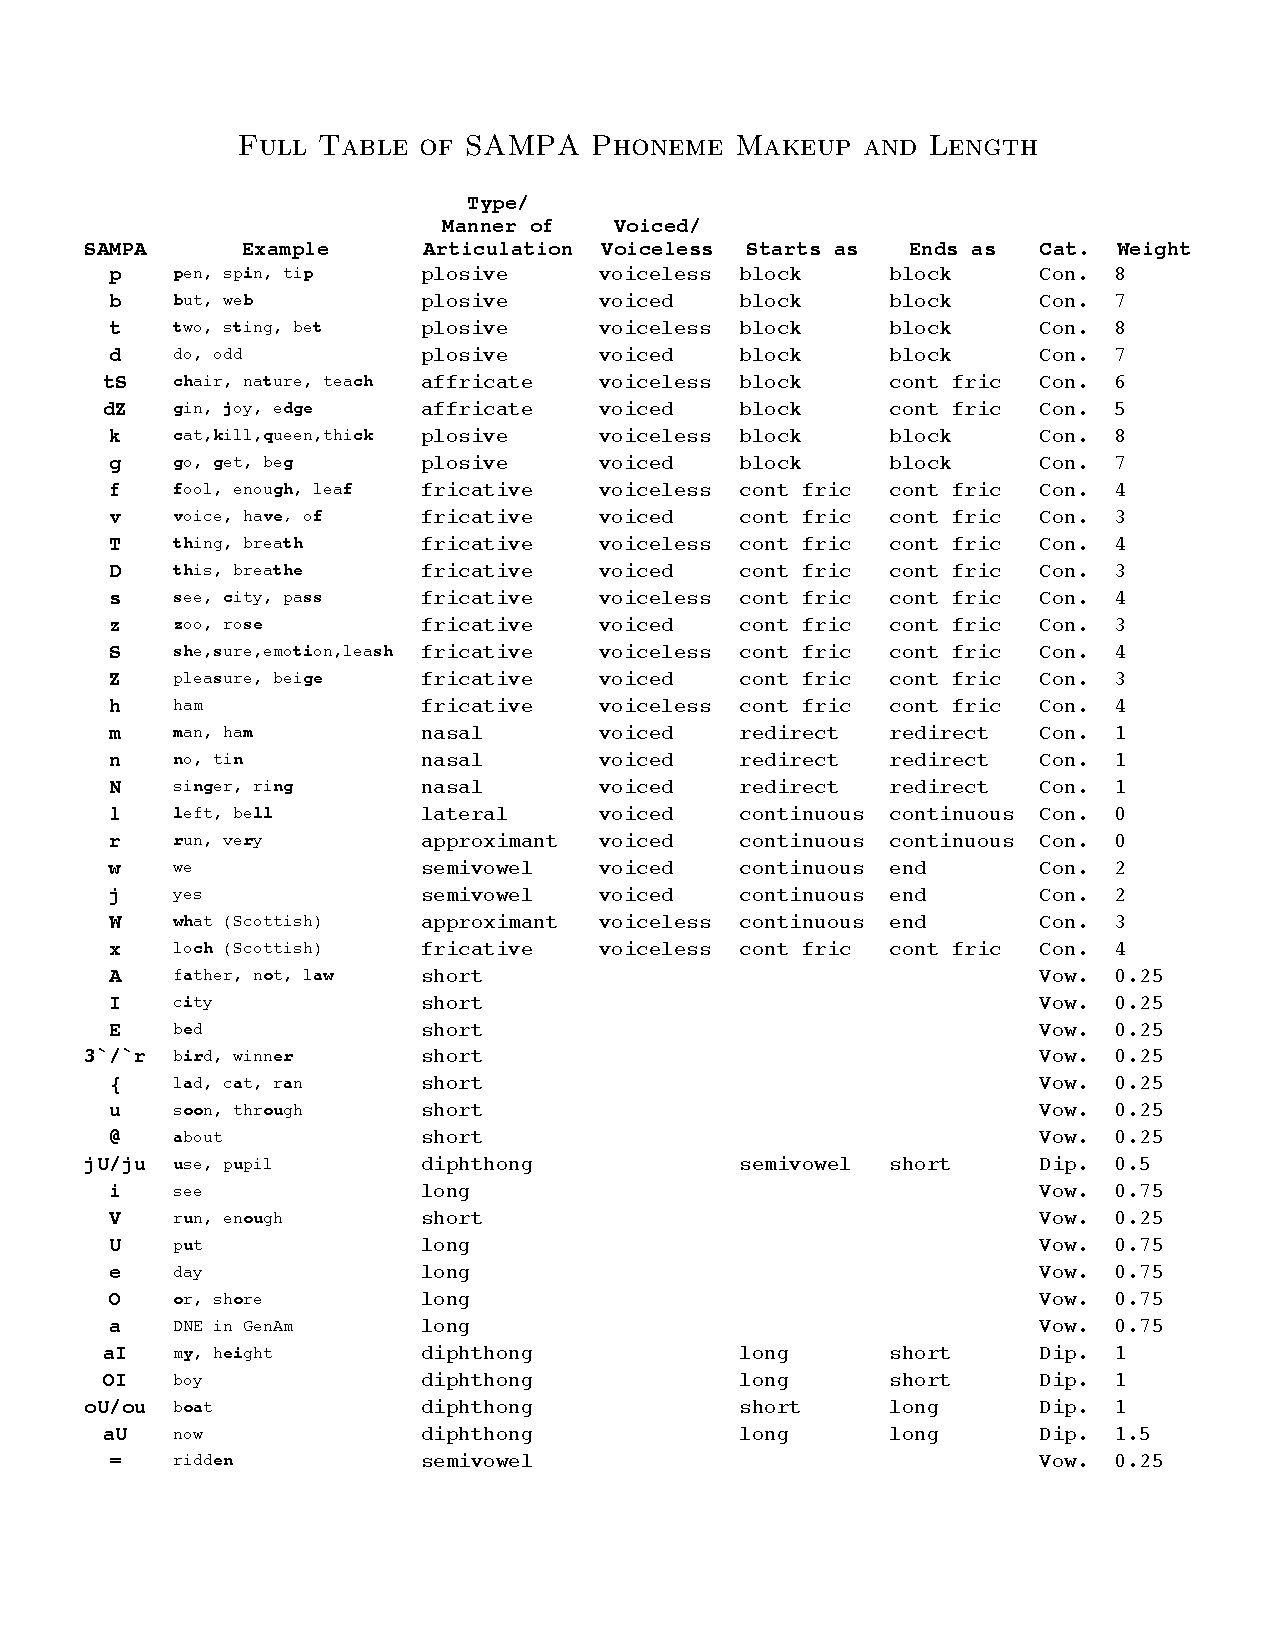
\includepdf[pages={-}]{AppendixSAMPATable.pdf}


\chapter{User Study Details}
\label{appendix:UserStudyDetails}



\label{table:phrasesRecorded}

\begin{center}

%\begin{table}

\begin{longtable}{|c|c|c|}
\caption[Phrases Recorded]{Here are the phrases we recorded, how many times they were recorded, and the identifiers we used for each phrase}
\label{table:phrasesRecorded} 

\hline 
orthoPhrase & numRecordings & phraseID \\
\endfirsthead

\multicolumn{3}{c}%
{{\bfseries \tablename\ \thetable{} -- continued from previous page}} \\
\hline
orthoPhrase & numRecordings & phraseID \\
\endhead


\hline \multicolumn{3}{|r|}{{Continued on next page}} \\ \hline
\endfoot

\hline \hline
\endlastfoot

\hline
a nice cold our   & 3 & A.17.51    a nice cold our  \\
\hline
an ice cold our   & 2 & A.17.135    an ice cold our  \\
\hline 
a nye scold our   & 2 & A.17.69    a nye scold our  \\
\hline 
ah nye scold our   & 2 & A.18.109    ah nye scold our  \\
\hline 
an eye scold our   & 2 & A.18.125    an eye scold our  \\
\hline 
on aye scold our   & 2 & A.18.267    on aye scold our  \\
\hline 
a nigh scold our   & 2 & A.18.65    a nigh scold our  \\
\hline 
a nye skol dower   & 2 & A.18.71    a nye skol dower  \\
\hline 
an aye skol dower   & 2 & A.19.119    an aye skol dower  \\
\hline 
an eye skol dower   & 2 & A.19.127    an eye skol dower  \\
\hline 
an ice coal dower   & 2 & A.19.133    an ice coal dower  \\
\hline 
eh nice coal dower   & 2 & A.20.159    eh nice coal dower  \\
\hline 
ah nice coal dower   & 2 & A.20.89    ah nice coal dower  \\
\hline 
fourth wry to   & 2 & B.15.19    fourth wry to  \\
\hline 
fourth wry too   & 2 & B.16.20    fourth wry too  \\
\hline 
forth right ooh   & 2 & B.17.1    forth right ooh  \\
\hline 
fourth rite ooh   & 2 & B.17.13    fourth rite ooh  \\
\hline 
forth wright ooh   & 2 & B.18.6    forth wright ooh  \\
\hline 
on i scold our   & 1 & A.16.279    on i scold our  \\
\hline 
an i scold hour   & 1 & A.17.128    an i scold hour  \\
\hline 
an i skol dower   & 1 & A.17.131    an i skol dower  \\
\hline 
an ice-cold our   & 1 & A.17.141    an ice-cold our  \\
\hline 
on i scold hour   & 1 & A.17.278    on i scold hour  \\
\hline 
on i skol dower   & 1 & A.17.281    on i skol dower  \\
\hline 
an aye scold our   & 1 & A.18.117    an aye scold our  \\
\hline 
an ice cold hour   & 1 & A.18.134    an ice cold hour  \\
\hline 
an ice-cold hour   & 1 & A.18.140    an ice-cold hour  \\
\hline 
eh nye scold our   & 1 & A.18.179    eh nye scold our  \\
\hline 
on eye scold our   & 1 & A.18.275    on eye scold our  \\
\hline 
on ice cold hour   & 1 & A.18.284    on ice cold hour  \\
\hline 
on ice-cold hour   & 1 & A.18.290    on ice-cold hour  \\
\hline 
a nye scold hour   & 1 & A.18.68    a nye scold hour  \\
\hline 
ah nice cold our   & 1 & A.18.91    ah nice cold our  \\
\hline 
ah nigh scold our   & 1 & A.19.105    ah nigh scold our  \\
\hline 
ah nye scold hour   & 1 & A.19.108    ah nye scold hour  \\
\hline 
ah nye skol dower   & 1 & A.19.111    ah nye skol dower  \\
\hline 
an aye scold hour   & 1 & A.19.116    an aye scold hour  \\
\hline 
an ice kohl dower   & 1 & A.19.139    an ice kohl dower  \\
\hline 
eh nice cold hour   & 1 & A.19.160    eh nice cold hour  \\
\hline 
eh nigh scold our   & 1 & A.19.175    eh nigh scold our  \\
\hline 
eh nye skol dower   & 1 & A.19.181    eh nye skol dower  \\
\hline 
on aye skol dower   & 1 & A.19.269    on aye skol dower  \\
\hline 
on eye scold hour   & 1 & A.19.274    on eye scold hour  \\
\hline 
on ice coal dower   & 1 & A.19.283    on ice coal dower  \\
\hline 
on ice kohl dower   & 1 & A.19.289    on ice kohl dower  \\
\hline 
a nice coal dower   & 1 & A.19.49    a nice coal dower  \\
\hline 
a nigh scold hour   & 1 & A.19.64    a nigh scold hour  \\
\hline 
ah nice cold hour   & 1 & A.19.90    ah nice cold hour  \\
\hline 
eh nice cole dower   & 1 & A.20.163    eh nice cole dower  \\
\hline 
eh nigh scold hour   & 1 & A.20.174    eh nigh scold hour  \\
\hline 
eh nigh skol dower   & 1 & A.20.177    eh nigh skol dower  \\
\hline 
ah nice cole dower   & 1 & A.20.93    ah nice cole dower  \\
\hline 
ah nice kohl dower   & 1 & A.20.95    ah nice kohl dower  \\
\hline 
forth wry two   & 1 & B.15.10    forth wry two  \\
\hline 
forth rye two   & 1 & B.15.5    forth rye two  \\
\hline 
forth write ooh   & 1 & B.17.7    forth write ooh  \\
\hline 
fourth right ooh   & 1 & B.18.12    fourth right ooh  \\
\hline 
fourth wright ooh   & 1 & B.19.17    fourth wright ooh  \\
\hline

\end{longtable}

%\end{table}
\end{center}



\begin{table}
\begin{center}

\begin{tabular}{|c|c|c|}
\hline 
Response By Country   &   Num Responses   \\ \hline
USA   &   506   \\ \hline
India   &   277   \\ \hline
Canada   &   33   \\ \hline
England   &   28   \\ \hline
Macedonia   &   28   \\ \hline
Washington   &   13   \\ \hline
Syria   &   13   \\ \hline
UK   &   11   \\ \hline
Sri Lanka   &   7   \\ \hline
Britain   &   4   \\ \hline
Vietnam   &   4   \\ \hline
Egypt   &   3   \\ \hline
Finland   &   3   \\ \hline
Iran   &   3   \\ \hline
Phillipines   &   3   \\ \hline
The Netherlands   &   2   \\ \hline
Mexico   &   2   \\ \hline
``english''   &   2   \\ \hline
Belgium   &   2   \\ \hline
Ireland   &   2   \\ \hline
Other   &   8   \\ \hline
%South Africa   &   1   \\ \hline
%West Indies   &   1   \\ \hline
%Brazil   &   1   \\ \hline
%Uruguay   &   1   \\ \hline
%Turkey   &   1   \\ \hline
%Bangladesh   &   1   \\ \hline
%Trinidad and Tobago   &   1   \\ \hline
%China   &   1   \\ \hline
\end{tabular}

\captionfonts
\caption[Countries and responses]{ Here's a table with the number of responses per country}
\label{table:countryTally}
\end{center}
\end{table}



%\include{table:phrasesRecorded}

%\label{phaseOneBubbleCharts}
\section{Individual Recording/Transcription Breakdowns}
These are recording-by-recording transcription breakdowns for phase one of our user study. Each bubble charts represent the most common transcriptions for the recorded phrase listed at the top. The size of the bubble and the position along the x axis is indicative of the number of times that phrase was transcribed for this particular recording.  The position along the y axis shows how often this phrase was transcribed over all the recordings.

Note that, for the purposes of clarifying these graphs, we did not chart any anomalous transcriptions--that is, transcriptions with only one occurance in this recording, or transcriptions with less than 5 percent of the recording's transcriptions with no other occurances over the entire set of recordings.  Doing so did not give us useful visual data, because the bubbles stacked and obscured eachother.  A full table of the transcriptions per recorded phrase can be provided upon request.





\def \piechartwidth { 75mm }

\begin{figure}[h]
\begin{center}
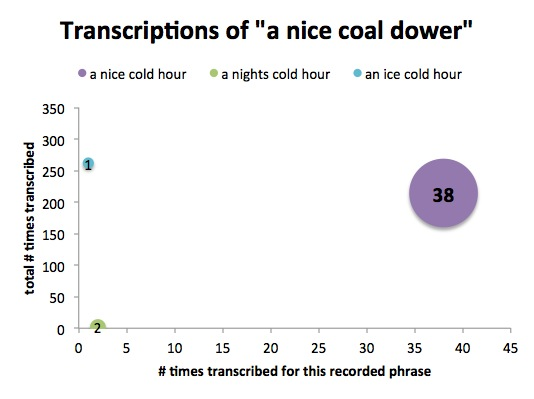
\includegraphics[width=\piechartwidth]{bubbleChartTranscriptionFrequency_aNiceCoalDower.jpg}
\captionfonts
\caption[Most common transcriptions for the recorded phrase "a nice coal dower"]{}
\label{bubbleChart:aNiceCoalDower}
\end{center}
\end{figure}


\begin{figure}[h]
\begin{center}
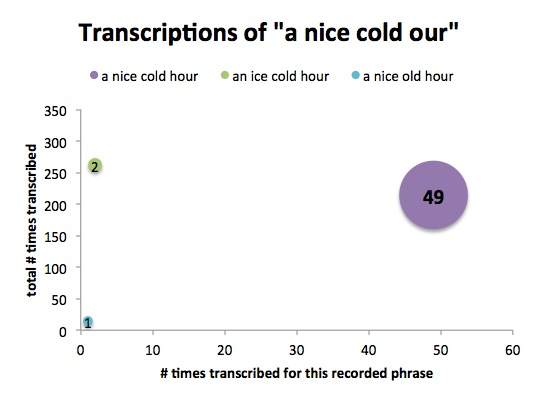
\includegraphics[width=\piechartwidth]{bubbleChartTranscriptionFrequency_aNiceColdOur.jpg}
\captionfonts
\caption[Most common transcriptions for the recorded phrase "aNiceColdOur"]{}
\label{bubbleChart:aNiceColdOur}
\end{center}
\end{figure}



\begin{figure}[h]
\begin{center}
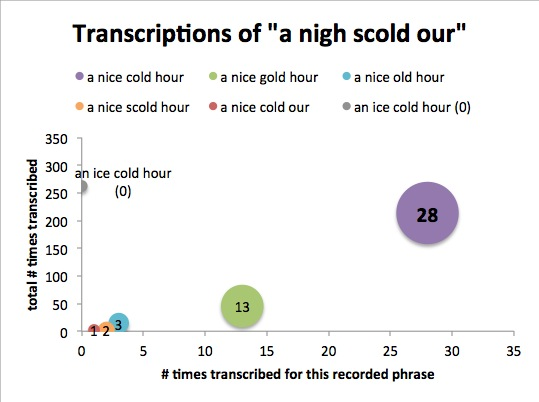
\includegraphics[width=\piechartwidth]{bubbleChartTranscriptionFrequency_aNighScoldOur.jpg}
\captionfonts
\caption[Most common transcriptions for the recorded phrase "aNighScoldOur"]{}
\label{bubbleChart:aNighScoldOur}
\end{center}
\end{figure}

\begin{figure}[h]
\begin{center}
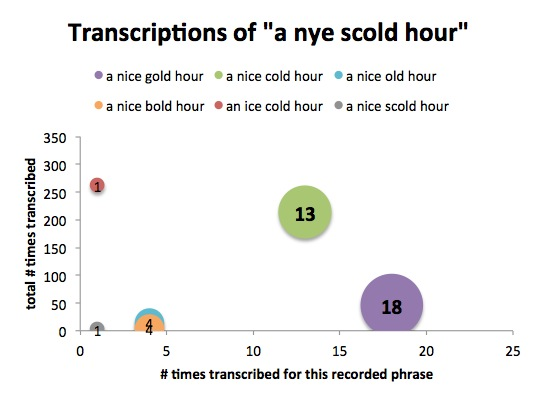
\includegraphics[width=\piechartwidth]{bubbleChartTranscriptionFrequency_aNyeScoldHour.jpg}
\captionfonts
\caption[Most common transcriptions for the recorded phrase "aNyeScoldHour"]{}
\label{bubbleChart:aNyeScoldHour}
\end{center}
\end{figure}

\begin{figure}[h]
\begin{center}
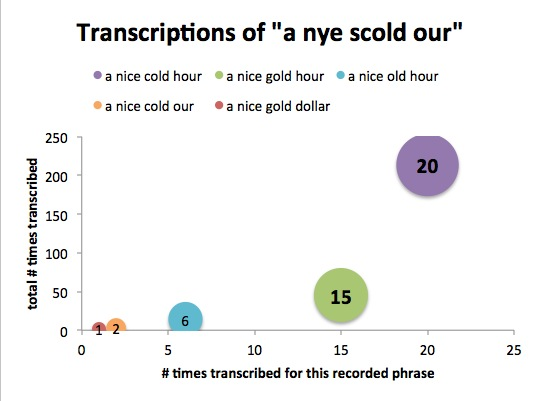
\includegraphics[width=\piechartwidth]{bubbleChartTranscriptionFrequency_aNyeScoldOur.jpg}
\captionfonts
\caption[Most common transcriptions for the recorded phrase "aNyeScoldOur"]{}
\label{bubbleChart:aNyeScoldOur}
\end{center}
\end{figure}

\begin{figure}[h]
\begin{center}
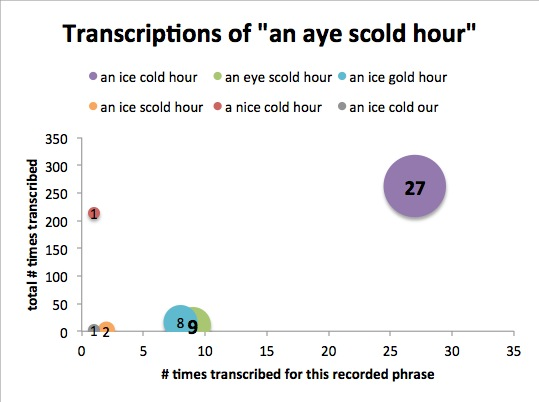
\includegraphics[width=\piechartwidth]{bubbleChartTranscriptionFrequency_anAyeScoldHour.jpg}
\captionfonts
\caption[Most common transcriptions for the recorded phrase "anAyeScoldHour"]{}
\label{bubbleChart:anAyeScoldHour}
\end{center}
\end{figure}

\begin{figure}[h]
\begin{center}
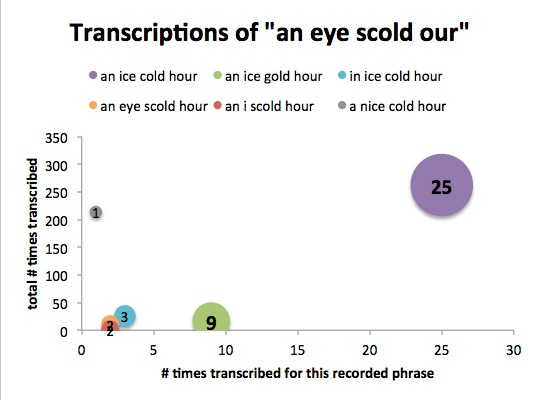
\includegraphics[width=\piechartwidth]{bubbleChartTranscriptionFrequency_anEyeScoldOur.jpg}
\captionfonts
\caption[Most common transcriptions for the recorded phrase "anEyeScoldOur"]{}
\label{bubbleChart:anEyeScoldOur}
\end{center}
\end{figure}

\begin{figure}[h]
\begin{center}
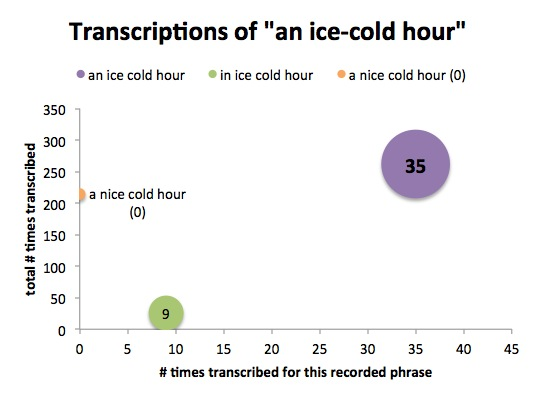
\includegraphics[width=\piechartwidth]{bubbleChartTranscriptionFrequency_anIce-ColdHour.jpg}
\captionfonts
\caption[Most common transcriptions for the recorded phrase "an Ice-Cold Hour"]{}
\label{bubbleChart:anIce-ColdHour}
\end{center}
\end{figure}

\begin{figure}[h]
\begin{center}
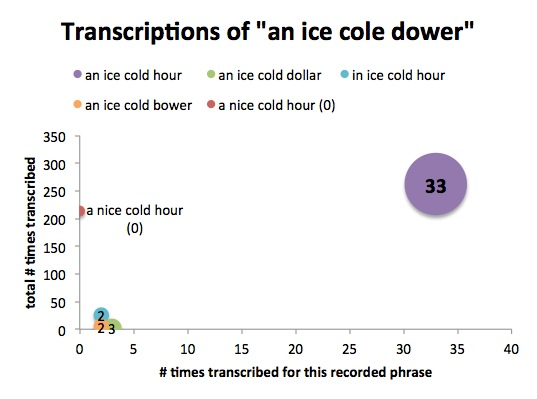
\includegraphics[width=\piechartwidth]{bubbleChartTranscriptionFrequency_anIceColeDower.jpg}
\captionfonts
\caption[Most common transcriptions for the recorded phrase "anIceColeDower"]{}
\label{bubbleChart:anIceColeDower}
\end{center}
\end{figure}

\begin{figure}[h]
\begin{center}
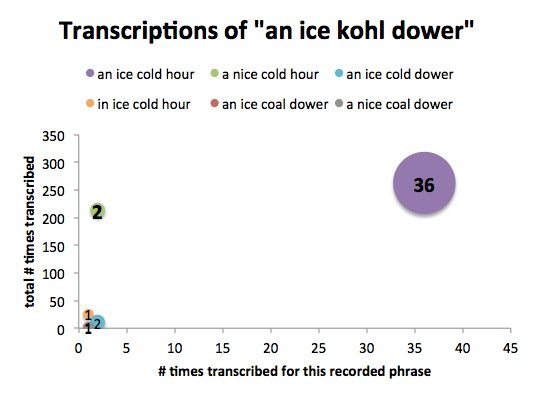
\includegraphics[width=\piechartwidth]{bubbleChartTranscriptionFrequency_anIceKohlDower.jpg}
\captionfonts
\caption[Most common transcriptions for the recorded phrase "anIceKohlDower"]{}
\label{bubbleChart:anIceKohlDower}
\end{center}
\end{figure}

\begin{figure}[h]
\begin{center}
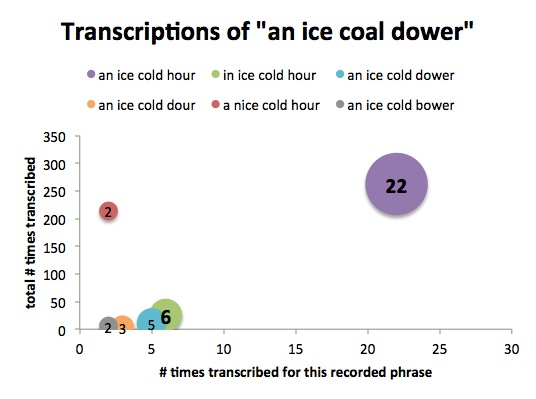
\includegraphics[width=\piechartwidth]{bubbleChartTranscriptionFrequency_an_IceCoalDower.jpg}
\captionfonts
\caption[Most common transcriptions for the recorded phrase "an_IceCoalDower"]{}
\label{bubbleChart:an_IceCoalDower}
\end{center}
\end{figure}

\begin{figure}[h]
\begin{center}
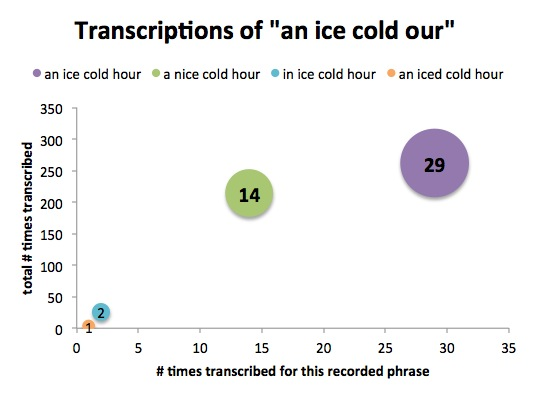
\includegraphics[width=\piechartwidth]{bubbleChartTranscriptionFrequency_an_iceColdOur.jpg}
\captionfonts
\caption[Most common transcriptions for the recorded phrase "a NiceColdOur"]{}
\label{bubbleChart:an_niceColdOur}
\end{center}
\end{figure}

\begin{figure}[h]
\begin{center}
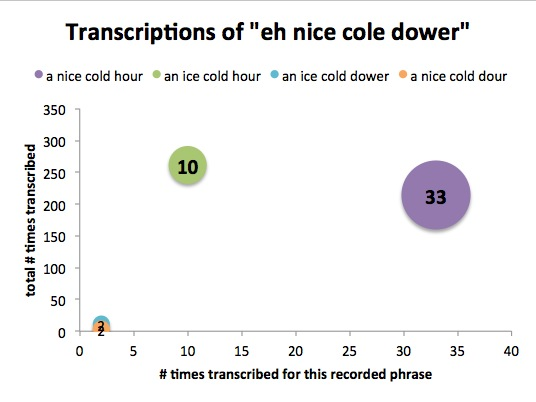
\includegraphics[width=\piechartwidth]{bubbleChartTranscriptionFrequency_ehNiceColeDower.jpg}
\captionfonts
\caption[Most common transcriptions for the recorded phrase "ehNiceColeDower"]{}
\label{bubbleChart:ehNiceColeDower}
\end{center}
\end{figure}


  
\begin{figure}[h]
\begin{center}
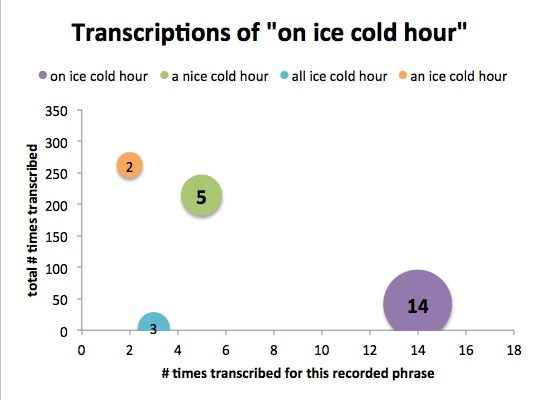
\includegraphics[width=\piechartwidth]{bubbleChartTranscriptionFrequency_onIceColdHour.jpg}
\captionfonts
\caption[Most common transcriptions for the recorded phrase "onIceColdHour"]{This phonetic sequence deterministically parses to the word ``on".  Unsurprisingly, in all recording with the word ``on", it was nearly always heard and trascribed as ``on"}
\label{bubbleChart:onIceColdHour}
\end{center}
\end{figure}

\begin{figure}[h]
\begin{center}
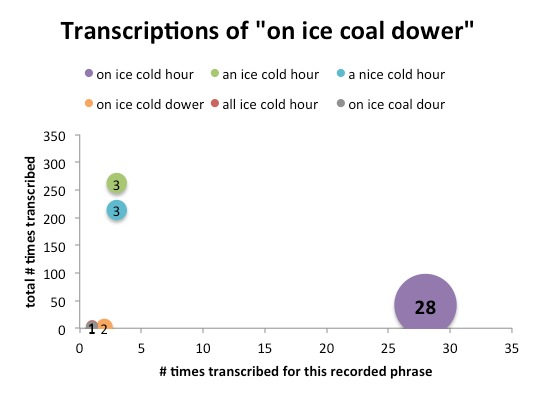
\includegraphics[width=\piechartwidth]{bubbleChartTranscriptionFrequency_onIceCoalDower.jpg}
\captionfonts
\caption[Most common transcriptions for the recorded phrase "onIceCoalDower"]{This phonetic sequence deterministically parses to the word ``on".  Unsurprisingly, in all recording with the word ``on", it was nearly always heard and trascribed as ``on"}
\label{bubbleChart:onIceCoalDower}
\end{center}
\end{figure}
%\setlength\LTleft{-1in}


\begin {longtable}{ cc|cccccccc }
\caption[All Oronyms for `A Nice Cold Hour' with frequency values]{All Oronyms for `A Nice Cold Hour' with frequency values}
\global\label{table:aNiceColdHourOronymWithFreqsTable}

\hline
phrase  &   total freq  &  word1  &  freq1  &  word2  &  freq2  &  word3  &  freq3  &  word4  &  freq4   \\ \hline
\endfirsthead

\multicolumn{10}{c}%
{{\bfseries \tablename\ \thetable{} -- continued from previous page}} \\
\hline
phrase  &   total freq  &  word1  &  freq1  &  word2  &  freq2  &  word3  &  freq3  &  word4  &  freq4   \\ \hline
\endhead

\hline \multicolumn{10}{|r|}{{Continued on next page}} \\ \hline
\endfoot

\hline \hline
\endlastfoot

 on i scold our   &  13185760  &   on   &  2774243  &   i   &  9937877  &   scold   &  217  &   our   &  473423   \\ \hline
 on i scold hour   &  12784150  &   on   &  2774243  &   i   &  9937877  &   scold   &  217  &   hour   &  71813   \\ \hline
 on i skol dour   &  12712244  &   on   &  2774243  &   i   &  9937877  &   skol   &  5  &   dour   &  119   \\ \hline
 on i skol dower   &  12712217  &   on   &  2774243  &   i   &  9937877  &   skol   &  5  &   dower   &  92   \\ \hline
 an i scold our   &  11205686  &   an   &  794169  &   i   &  9937877  &   scold   &  217  &   our   &  473423   \\ \hline
 an i scold hour   &  10804076  &   an   &  794169  &   i   &  9937877  &   scold   &  217  &   hour   &  71813   \\ \hline
 an i skol dour   &  10732170  &   an   &  794169  &   i   &  9937877  &   skol   &  5  &   dour   &  119   \\ \hline
 an i skol dower   &  10732143  &   an   &  794169  &   i   &  9937877  &   skol   &  5  &   dower   &  92   \\ \hline
 'n' i scold our   &  10411517  &   'n'   &  0  &   i   &  9937877  &   scold   &  217  &   our   &  473423   \\ \hline
 'n' i scold hour   &  10009907  &   'n'   &  0  &   i   &  9937877  &   scold   &  217  &   hour   &  71813   \\ \hline
 'n' i skol dour   &  9938001  &   'n'   &  0  &   i   &  9937877  &   skol   &  5  &   dour   &  119   \\ \hline
 'n' i skol dower   &  9937974  &   'n'   &  0  &   i   &  9937877  &   skol   &  5  &   dower   &  92   \\ \hline
 a nice cold our   &  8253272  &   a   &  7536297  &   nice   &  190708  &   cold   &  52844  &   our   &  473423   \\ \hline
 a niece cold our   &  8064257  &   a   &  7536297  &   niece   &  1693  &   cold   &  52844  &   our   &  473423   \\ \hline
 a gneiss cold our   &  8062585  &   a   &  7536297  &   gneiss   &  21  &   cold   &  52844  &   our   &  473423   \\ \hline
 a ne scold our   &  8017040  &   a   &  7536297  &   ne   &  7103  &   scold   &  217  &   our   &  473423   \\ \hline
 a knee scold our   &  8016076  &   a   &  7536297  &   knee   &  6139  &   scold   &  217  &   our   &  473423   \\ \hline
 a nigh scold our   &  8011331  &   a   &  7536297  &   nigh   &  1394  &   scold   &  217  &   our   &  473423   \\ \hline
 a nye scold our   &  8009974  &   a   &  7536297  &   nye   &  37  &   scold   &  217  &   our   &  473423   \\ \hline
 a nice cold hour   &  7851662  &   a   &  7536297  &   nice   &  190708  &   cold   &  52844  &   hour   &  71813   \\ \hline
 a nice coal dour   &  7747572  &   a   &  7536297  &   nice   &  190708  &   coal   &  20448  &   dour   &  119   \\ \hline
 a nice coal dower   &  7747545  &   a   &  7536297  &   nice   &  190708  &   coal   &  20448  &   dower   &  92   \\ \hline
 a nice cole dour   &  7729197  &   a   &  7536297  &   nice   &  190708  &   cole   &  2073  &   dour   &  119   \\ \hline
 a nice cole dower   &  7729170  &   a   &  7536297  &   nice   &  190708  &   cole   &  2073  &   dower   &  92   \\ \hline
 a nice kohl dour   &  7728036  &   a   &  7536297  &   nice   &  190708  &   kohl   &  912  &   dour   &  119   \\ \hline
 a nice kohl dower   &  7728009  &   a   &  7536297  &   nice   &  190708  &   kohl   &  912  &   dower   &  92   \\ \hline
 a niece cold hour   &  7662647  &   a   &  7536297  &   niece   &  1693  &   cold   &  52844  &   hour   &  71813   \\ \hline
 a gneiss cold hour   &  7660975  &   a   &  7536297  &   gneiss   &  21  &   cold   &  52844  &   hour   &  71813   \\ \hline
 a ne scold hour   &  7615430  &   a   &  7536297  &   ne   &  7103  &   scold   &  217  &   hour   &  71813   \\ \hline
 a knee scold hour   &  7614466  &   a   &  7536297  &   knee   &  6139  &   scold   &  217  &   hour   &  71813   \\ \hline
 a nigh scold hour   &  7609721  &   a   &  7536297  &   nigh   &  1394  &   scold   &  217  &   hour   &  71813   \\ \hline
 a nye scold hour   &  7608364  &   a   &  7536297  &   nye   &  37  &   scold   &  217  &   hour   &  71813   \\ \hline
 a niece coal dour   &  7558557  &   a   &  7536297  &   niece   &  1693  &   coal   &  20448  &   dour   &  119   \\ \hline
 a niece coal dower   &  7558530  &   a   &  7536297  &   niece   &  1693  &   coal   &  20448  &   dower   &  92   \\ \hline
 a gneiss coal dour   &  7556885  &   a   &  7536297  &   gneiss   &  21  &   coal   &  20448  &   dour   &  119   \\ \hline
 a gneiss coal dower   &  7556858  &   a   &  7536297  &   gneiss   &  21  &   coal   &  20448  &   dower   &  92   \\ \hline
 a ne skol dour   &  7543524  &   a   &  7536297  &   ne   &  7103  &   skol   &  5  &   dour   &  119   \\ \hline
 a ne skol dower   &  7543497  &   a   &  7536297  &   ne   &  7103  &   skol   &  5  &   dower   &  92   \\ \hline
 a knee skol dour   &  7542560  &   a   &  7536297  &   knee   &  6139  &   skol   &  5  &   dour   &  119   \\ \hline
 a knee skol dower   &  7542533  &   a   &  7536297  &   knee   &  6139  &   skol   &  5  &   dower   &  92   \\ \hline
 a niece cole dour   &  7540182  &   a   &  7536297  &   niece   &  1693  &   cole   &  2073  &   dour   &  119   \\ \hline
 a niece cole dower   &  7540155  &   a   &  7536297  &   niece   &  1693  &   cole   &  2073  &   dower   &  92   \\ \hline
 a niece kohl dour   &  7539021  &   a   &  7536297  &   niece   &  1693  &   kohl   &  912  &   dour   &  119   \\ \hline
 a niece kohl dower   &  7538994  &   a   &  7536297  &   niece   &  1693  &   kohl   &  912  &   dower   &  92   \\ \hline
 a gneiss cole dour   &  7538510  &   a   &  7536297  &   gneiss   &  21  &   cole   &  2073  &   dour   &  119   \\ \hline
 a gneiss cole dower   &  7538483  &   a   &  7536297  &   gneiss   &  21  &   cole   &  2073  &   dower   &  92   \\ \hline
 a nigh skol dour   &  7537815  &   a   &  7536297  &   nigh   &  1394  &   skol   &  5  &   dour   &  119   \\ \hline
 a nigh skol dower   &  7537788  &   a   &  7536297  &   nigh   &  1394  &   skol   &  5  &   dower   &  92   \\ \hline
 a gneiss kohl dour   &  7537349  &   a   &  7536297  &   gneiss   &  21  &   kohl   &  912  &   dour   &  119   \\ \hline
 a gneiss kohl dower   &  7537322  &   a   &  7536297  &   gneiss   &  21  &   kohl   &  912  &   dower   &  92   \\ \hline
 a nye skol dour   &  7536458  &   a   &  7536297  &   nye   &  37  &   skol   &  5  &   dour   &  119   \\ \hline
 a nye skol dower   &  7536431  &   a   &  7536297  &   nye   &  37  &   skol   &  5  &   dower   &  92   \\ \hline
 on aye scold our   &  3378386  &   on   &  2774243  &   aye   &  130503  &   scold   &  217  &   our   &  473423   \\ \hline
 on e scold our   &  3356846  &   on   &  2774243  &   e   &  108963  &   scold   &  217  &   our   &  473423   \\ \hline
 on ice cold our   &  3312712  &   on   &  2774243  &   ice   &  12202  &   cold   &  52844  &   our   &  473423   \\ \hline
 on eye scold our   &  3274633  &   on   &  2774243  &   eye   &  26750  &   scold   &  217  &   our   &  473423   \\ \hline
 on ay scold our   &  3254516  &   on   &  2774243  &   ay   &  6633  &   scold   &  217  &   our   &  473423   \\ \hline
 on ice-cold our   &  3247715  &   on   &  2774243  &   ice-cold   &  49  &   our   &  473423  &     &     \\ \hline
 on aye scold hour   &  2976776  &   on   &  2774243  &   aye   &  130503  &   scold   &  217  &   hour   &  71813   \\ \hline
 on e scold hour   &  2955236  &   on   &  2774243  &   e   &  108963  &   scold   &  217  &   hour   &  71813   \\ \hline
 on ice cold hour   &  2911102  &   on   &  2774243  &   ice   &  12202  &   cold   &  52844  &   hour   &  71813   \\ \hline
 on aye skol dour   &  2904870  &   on   &  2774243  &   aye   &  130503  &   skol   &  5  &   dour   &  119   \\ \hline
 on aye skol dower   &  2904843  &   on   &  2774243  &   aye   &  130503  &   skol   &  5  &   dower   &  92   \\ \hline
 on e skol dour   &  2883330  &   on   &  2774243  &   e   &  108963  &   skol   &  5  &   dour   &  119   \\ \hline
 on e skol dower   &  2883303  &   on   &  2774243  &   e   &  108963  &   skol   &  5  &   dower   &  92   \\ \hline
 on eye scold hour   &  2873023  &   on   &  2774243  &   eye   &  26750  &   scold   &  217  &   hour   &  71813   \\ \hline
 on ay scold hour   &  2852906  &   on   &  2774243  &   ay   &  6633  &   scold   &  217  &   hour   &  71813   \\ \hline
 on ice-cold hour   &  2846105  &   on   &  2774243  &   ice-cold   &  49  &   hour   &  71813  &     &     \\ \hline
 on ice coal dour   &  2807012  &   on   &  2774243  &   ice   &  12202  &   coal   &  20448  &   dour   &  119   \\ \hline
 on ice coal dower   &  2806985  &   on   &  2774243  &   ice   &  12202  &   coal   &  20448  &   dower   &  92   \\ \hline
 on eye skol dour   &  2801117  &   on   &  2774243  &   eye   &  26750  &   skol   &  5  &   dour   &  119   \\ \hline
 on eye skol dower   &  2801090  &   on   &  2774243  &   eye   &  26750  &   skol   &  5  &   dower   &  92   \\ \hline
 on ice cole dour   &  2788637  &   on   &  2774243  &   ice   &  12202  &   cole   &  2073  &   dour   &  119   \\ \hline
 on ice cole dower   &  2788610  &   on   &  2774243  &   ice   &  12202  &   cole   &  2073  &   dower   &  92   \\ \hline
 on ice kohl dour   &  2787476  &   on   &  2774243  &   ice   &  12202  &   kohl   &  912  &   dour   &  119   \\ \hline
 on ice kohl dower   &  2787449  &   on   &  2774243  &   ice   &  12202  &   kohl   &  912  &   dower   &  92   \\ \hline
 on ay skol dour   &  2781000  &   on   &  2774243  &   ay   &  6633  &   skol   &  5  &   dour   &  119   \\ \hline
 on ay skol dower   &  2780973  &   on   &  2774243  &   ay   &  6633  &   skol   &  5  &   dower   &  92   \\ \hline
 an aye scold our   &  1398312  &   an   &  794169  &   aye   &  130503  &   scold   &  217  &   our   &  473423   \\ \hline
 an e scold our   &  1376772  &   an   &  794169  &   e   &  108963  &   scold   &  217  &   our   &  473423   \\ \hline
 an ice cold our   &  1332638  &   an   &  794169  &   ice   &  12202  &   cold   &  52844  &   our   &  473423   \\ \hline
 an eye scold our   &  1294559  &   an   &  794169  &   eye   &  26750  &   scold   &  217  &   our   &  473423   \\ \hline
 an ay scold our   &  1274442  &   an   &  794169  &   ay   &  6633  &   scold   &  217  &   our   &  473423   \\ \hline
 an ice-cold our   &  1267641  &   an   &  794169  &   ice-cold   &  49  &   our   &  473423  &     &     \\ \hline
 an aye scold hour   &  996702  &   an   &  794169  &   aye   &  130503  &   scold   &  217  &   hour   &  71813   \\ \hline
 an e scold hour   &  975162  &   an   &  794169  &   e   &  108963  &   scold   &  217  &   hour   &  71813   \\ \hline
 ah nice cold our   &  946271  &   ah   &  229296  &   nice   &  190708  &   cold   &  52844  &   our   &  473423   \\ \hline
 an ice cold hour   &  931028  &   an   &  794169  &   ice   &  12202  &   cold   &  52844  &   hour   &  71813   \\ \hline
 an aye skol dour   &  924796  &   an   &  794169  &   aye   &  130503  &   skol   &  5  &   dour   &  119   \\ \hline
 an aye skol dower   &  924769  &   an   &  794169  &   aye   &  130503  &   skol   &  5  &   dower   &  92   \\ \hline
 an e skol dour   &  903256  &   an   &  794169  &   e   &  108963  &   skol   &  5  &   dour   &  119   \\ \hline
 an e skol dower   &  903229  &   an   &  794169  &   e   &  108963  &   skol   &  5  &   dower   &  92   \\ \hline
 an eye scold hour   &  892949  &   an   &  794169  &   eye   &  26750  &   scold   &  217  &   hour   &  71813   \\ \hline
 an ay scold hour   &  872832  &   an   &  794169  &   ay   &  6633  &   scold   &  217  &   hour   &  71813   \\ \hline
 an ice-cold hour   &  866031  &   an   &  794169  &   ice-cold   &  49  &   hour   &  71813  &     &     \\ \hline
 an ice coal dour   &  826938  &   an   &  794169  &   ice   &  12202  &   coal   &  20448  &   dour   &  119   \\ \hline
 an ice coal dower   &  826911  &   an   &  794169  &   ice   &  12202  &   coal   &  20448  &   dower   &  92   \\ \hline
 an eye skol dour   &  821043  &   an   &  794169  &   eye   &  26750  &   skol   &  5  &   dour   &  119   \\ \hline
 an eye skol dower   &  821016  &   an   &  794169  &   eye   &  26750  &   skol   &  5  &   dower   &  92   \\ \hline
 an ice cole dour   &  808563  &   an   &  794169  &   ice   &  12202  &   cole   &  2073  &   dour   &  119   \\ \hline
 an ice cole dower   &  808536  &   an   &  794169  &   ice   &  12202  &   cole   &  2073  &   dower   &  92   \\ \hline
 an ice kohl dour   &  807402  &   an   &  794169  &   ice   &  12202  &   kohl   &  912  &   dour   &  119   \\ \hline
 an ice kohl dower   &  807375  &   an   &  794169  &   ice   &  12202  &   kohl   &  912  &   dower   &  92   \\ \hline
 an ay skol dour   &  800926  &   an   &  794169  &   ay   &  6633  &   skol   &  5  &   dour   &  119   \\ \hline
 an ay skol dower   &  800899  &   an   &  794169  &   ay   &  6633  &   skol   &  5  &   dower   &  92   \\ \hline
 eh nice cold our   &  783938  &   eh   &  66963  &   nice   &  190708  &   cold   &  52844  &   our   &  473423   \\ \hline
 ah niece cold our   &  757256  &   ah   &  229296  &   niece   &  1693  &   cold   &  52844  &   our   &  473423   \\ \hline
 ah gneiss cold our   &  755584  &   ah   &  229296  &   gneiss   &  21  &   cold   &  52844  &   our   &  473423   \\ \hline
 et nice cold our   &  723706  &   et   &  6731  &   nice   &  190708  &   cold   &  52844  &   our   &  473423   \\ \hline
 o' nice cold our   &  717438  &   o'   &  463  &   nice   &  190708  &   cold   &  52844  &   our   &  473423   \\ \hline
 ah ne scold our   &  710039  &   ah   &  229296  &   ne   &  7103  &   scold   &  217  &   our   &  473423   \\ \hline
 ah knee scold our   &  709075  &   ah   &  229296  &   knee   &  6139  &   scold   &  217  &   our   &  473423   \\ \hline
 ah nigh scold our   &  704330  &   ah   &  229296  &   nigh   &  1394  &   scold   &  217  &   our   &  473423   \\ \hline
 ah nye scold our   &  702973  &   ah   &  229296  &   nye   &  37  &   scold   &  217  &   our   &  473423   \\ \hline
 'n' aye scold our   &  604143  &   'n'   &  0  &   aye   &  130503  &   scold   &  217  &   our   &  473423   \\ \hline
 eh niece cold our   &  594923  &   eh   &  66963  &   niece   &  1693  &   cold   &  52844  &   our   &  473423   \\ \hline
 eh gneiss cold our   &  593251  &   eh   &  66963  &   gneiss   &  21  &   cold   &  52844  &   our   &  473423   \\ \hline
 'n' e scold our   &  582603  &   'n'   &  0  &   e   &  108963  &   scold   &  217  &   our   &  473423   \\ \hline
 eh ne scold our   &  547706  &   eh   &  66963  &   ne   &  7103  &   scold   &  217  &   our   &  473423   \\ \hline
 eh knee scold our   &  546742  &   eh   &  66963  &   knee   &  6139  &   scold   &  217  &   our   &  473423   \\ \hline
 ah nice cold hour   &  544661  &   ah   &  229296  &   nice   &  190708  &   cold   &  52844  &   hour   &  71813   \\ \hline
 eh nigh scold our   &  541997  &   eh   &  66963  &   nigh   &  1394  &   scold   &  217  &   our   &  473423   \\ \hline
 eh nye scold our   &  540640  &   eh   &  66963  &   nye   &  37  &   scold   &  217  &   our   &  473423   \\ \hline
 'n' ice cold our   &  538469  &   'n'   &  0  &   ice   &  12202  &   cold   &  52844  &   our   &  473423   \\ \hline
 et niece cold our   &  534691  &   et   &  6731  &   niece   &  1693  &   cold   &  52844  &   our   &  473423   \\ \hline
 et gneiss cold our   &  533019  &   et   &  6731  &   gneiss   &  21  &   cold   &  52844  &   our   &  473423   \\ \hline
 o' niece cold our   &  528423  &   o'   &  463  &   niece   &  1693  &   cold   &  52844  &   our   &  473423   \\ \hline
 o' gneiss cold our   &  526751  &   o'   &  463  &   gneiss   &  21  &   cold   &  52844  &   our   &  473423   \\ \hline
 'n' eye scold our   &  500390  &   'n'   &  0  &   eye   &  26750  &   scold   &  217  &   our   &  473423   \\ \hline
 et ne scold our   &  487474  &   et   &  6731  &   ne   &  7103  &   scold   &  217  &   our   &  473423   \\ \hline
 et knee scold our   &  486510  &   et   &  6731  &   knee   &  6139  &   scold   &  217  &   our   &  473423   \\ \hline
 et nigh scold our   &  481765  &   et   &  6731  &   nigh   &  1394  &   scold   &  217  &   our   &  473423   \\ \hline
 o' ne scold our   &  481206  &   o'   &  463  &   ne   &  7103  &   scold   &  217  &   our   &  473423   \\ \hline
 et nye scold our   &  480408  &   et   &  6731  &   nye   &  37  &   scold   &  217  &   our   &  473423   \\ \hline
 'n' ay scold our   &  480273  &   'n'   &  0  &   ay   &  6633  &   scold   &  217  &   our   &  473423   \\ \hline
 o' knee scold our   &  480242  &   o'   &  463  &   knee   &  6139  &   scold   &  217  &   our   &  473423   \\ \hline
 o' nigh scold our   &  475497  &   o'   &  463  &   nigh   &  1394  &   scold   &  217  &   our   &  473423   \\ \hline
 o' nye scold our   &  474140  &   o'   &  463  &   nye   &  37  &   scold   &  217  &   our   &  473423   \\ \hline
 'n' ice-cold our   &  473472  &   'n'   &  0  &   ice-cold   &  49  &   our   &  473423  &     &     \\ \hline
 ah nice coal dour   &  440571  &   ah   &  229296  &   nice   &  190708  &   coal   &  20448  &   dour   &  119   \\ \hline
 ah nice coal dower   &  440544  &   ah   &  229296  &   nice   &  190708  &   coal   &  20448  &   dower   &  92   \\ \hline
 ah nice cole dour   &  422196  &   ah   &  229296  &   nice   &  190708  &   cole   &  2073  &   dour   &  119   \\ \hline
 ah nice cole dower   &  422169  &   ah   &  229296  &   nice   &  190708  &   cole   &  2073  &   dower   &  92   \\ \hline
 ah nice kohl dour   &  421035  &   ah   &  229296  &   nice   &  190708  &   kohl   &  912  &   dour   &  119   \\ \hline
 ah nice kohl dower   &  421008  &   ah   &  229296  &   nice   &  190708  &   kohl   &  912  &   dower   &  92   \\ \hline
 eh nice cold hour   &  382328  &   eh   &  66963  &   nice   &  190708  &   cold   &  52844  &   hour   &  71813   \\ \hline
 ah niece cold hour   &  355646  &   ah   &  229296  &   niece   &  1693  &   cold   &  52844  &   hour   &  71813   \\ \hline
 ah gneiss cold hour   &  353974  &   ah   &  229296  &   gneiss   &  21  &   cold   &  52844  &   hour   &  71813   \\ \hline
 et nice cold hour   &  322096  &   et   &  6731  &   nice   &  190708  &   cold   &  52844  &   hour   &  71813   \\ \hline
 o' nice cold hour   &  315828  &   o'   &  463  &   nice   &  190708  &   cold   &  52844  &   hour   &  71813   \\ \hline
 ah ne scold hour   &  308429  &   ah   &  229296  &   ne   &  7103  &   scold   &  217  &   hour   &  71813   \\ \hline
 ah knee scold hour   &  307465  &   ah   &  229296  &   knee   &  6139  &   scold   &  217  &   hour   &  71813   \\ \hline
 ah nigh scold hour   &  302720  &   ah   &  229296  &   nigh   &  1394  &   scold   &  217  &   hour   &  71813   \\ \hline
 ah nye scold hour   &  301363  &   ah   &  229296  &   nye   &  37  &   scold   &  217  &   hour   &  71813   \\ \hline
 eh nice coal dour   &  278238  &   eh   &  66963  &   nice   &  190708  &   coal   &  20448  &   dour   &  119   \\ \hline
 eh nice coal dower   &  278211  &   eh   &  66963  &   nice   &  190708  &   coal   &  20448  &   dower   &  92   \\ \hline
 eh nice cole dour   &  259863  &   eh   &  66963  &   nice   &  190708  &   cole   &  2073  &   dour   &  119   \\ \hline
 eh nice cole dower   &  259836  &   eh   &  66963  &   nice   &  190708  &   cole   &  2073  &   dower   &  92   \\ \hline
 eh nice kohl dour   &  258702  &   eh   &  66963  &   nice   &  190708  &   kohl   &  912  &   dour   &  119   \\ \hline
 eh nice kohl dower   &  258675  &   eh   &  66963  &   nice   &  190708  &   kohl   &  912  &   dower   &  92   \\ \hline
 ah niece coal dour   &  251556  &   ah   &  229296  &   niece   &  1693  &   coal   &  20448  &   dour   &  119   \\ \hline
 ah niece coal dower   &  251529  &   ah   &  229296  &   niece   &  1693  &   coal   &  20448  &   dower   &  92   \\ \hline
 ah gneiss coal dour   &  249884  &   ah   &  229296  &   gneiss   &  21  &   coal   &  20448  &   dour   &  119   \\ \hline
 ah gneiss coal dower   &  249857  &   ah   &  229296  &   gneiss   &  21  &   coal   &  20448  &   dower   &  92   \\ \hline
 ah ne skol dour   &  236523  &   ah   &  229296  &   ne   &  7103  &   skol   &  5  &   dour   &  119   \\ \hline
 ah ne skol dower   &  236496  &   ah   &  229296  &   ne   &  7103  &   skol   &  5  &   dower   &  92   \\ \hline
 ah knee skol dour   &  235559  &   ah   &  229296  &   knee   &  6139  &   skol   &  5  &   dour   &  119   \\ \hline
 ah knee skol dower   &  235532  &   ah   &  229296  &   knee   &  6139  &   skol   &  5  &   dower   &  92   \\ \hline
 ah niece cole dour   &  233181  &   ah   &  229296  &   niece   &  1693  &   cole   &  2073  &   dour   &  119   \\ \hline
 ah niece cole dower   &  233154  &   ah   &  229296  &   niece   &  1693  &   cole   &  2073  &   dower   &  92   \\ \hline
 ah niece kohl dour   &  232020  &   ah   &  229296  &   niece   &  1693  &   kohl   &  912  &   dour   &  119   \\ \hline
 ah niece kohl dower   &  231993  &   ah   &  229296  &   niece   &  1693  &   kohl   &  912  &   dower   &  92   \\ \hline
 ah gneiss cole dour   &  231509  &   ah   &  229296  &   gneiss   &  21  &   cole   &  2073  &   dour   &  119   \\ \hline
 ah gneiss cole dower   &  231482  &   ah   &  229296  &   gneiss   &  21  &   cole   &  2073  &   dower   &  92   \\ \hline
 ah nigh skol dour   &  230814  &   ah   &  229296  &   nigh   &  1394  &   skol   &  5  &   dour   &  119   \\ \hline
 ah nigh skol dower   &  230787  &   ah   &  229296  &   nigh   &  1394  &   skol   &  5  &   dower   &  92   \\ \hline
 ah gneiss kohl dour   &  230348  &   ah   &  229296  &   gneiss   &  21  &   kohl   &  912  &   dour   &  119   \\ \hline
 ah gneiss kohl dower   &  230321  &   ah   &  229296  &   gneiss   &  21  &   kohl   &  912  &   dower   &  92   \\ \hline
 ah nye skol dour   &  229457  &   ah   &  229296  &   nye   &  37  &   skol   &  5  &   dour   &  119   \\ \hline
 ah nye skol dower   &  229430  &   ah   &  229296  &   nye   &  37  &   skol   &  5  &   dower   &  92   \\ \hline
 et nice coal dour   &  218006  &   et   &  6731  &   nice   &  190708  &   coal   &  20448  &   dour   &  119   \\ \hline
 et nice coal dower   &  217979  &   et   &  6731  &   nice   &  190708  &   coal   &  20448  &   dower   &  92   \\ \hline
 o' nice coal dour   &  211738  &   o'   &  463  &   nice   &  190708  &   coal   &  20448  &   dour   &  119   \\ \hline
 o' nice coal dower   &  211711  &   o'   &  463  &   nice   &  190708  &   coal   &  20448  &   dower   &  92   \\ \hline
 'n' aye scold hour   &  202533  &   'n'   &  0  &   aye   &  130503  &   scold   &  217  &   hour   &  71813   \\ \hline
 et nice cole dour   &  199631  &   et   &  6731  &   nice   &  190708  &   cole   &  2073  &   dour   &  119   \\ \hline
 et nice cole dower   &  199604  &   et   &  6731  &   nice   &  190708  &   cole   &  2073  &   dower   &  92   \\ \hline
 et nice kohl dour   &  198470  &   et   &  6731  &   nice   &  190708  &   kohl   &  912  &   dour   &  119   \\ \hline
 et nice kohl dower   &  198443  &   et   &  6731  &   nice   &  190708  &   kohl   &  912  &   dower   &  92   \\ \hline
 o' nice cole dour   &  193363  &   o'   &  463  &   nice   &  190708  &   cole   &  2073  &   dour   &  119   \\ \hline
 o' nice cole dower   &  193336  &   o'   &  463  &   nice   &  190708  &   cole   &  2073  &   dower   &  92   \\ \hline
 eh niece cold hour   &  193313  &   eh   &  66963  &   niece   &  1693  &   cold   &  52844  &   hour   &  71813   \\ \hline
 o' nice kohl dour   &  192202  &   o'   &  463  &   nice   &  190708  &   kohl   &  912  &   dour   &  119   \\ \hline
 o' nice kohl dower   &  192175  &   o'   &  463  &   nice   &  190708  &   kohl   &  912  &   dower   &  92   \\ \hline
 eh gneiss cold hour   &  191641  &   eh   &  66963  &   gneiss   &  21  &   cold   &  52844  &   hour   &  71813   \\ \hline
 'n' e scold hour   &  180993  &   'n'   &  0  &   e   &  108963  &   scold   &  217  &   hour   &  71813   \\ \hline
 eh ne scold hour   &  146096  &   eh   &  66963  &   ne   &  7103  &   scold   &  217  &   hour   &  71813   \\ \hline
 eh knee scold hour   &  145132  &   eh   &  66963  &   knee   &  6139  &   scold   &  217  &   hour   &  71813   \\ \hline
 eh nigh scold hour   &  140387  &   eh   &  66963  &   nigh   &  1394  &   scold   &  217  &   hour   &  71813   \\ \hline
 eh nye scold hour   &  139030  &   eh   &  66963  &   nye   &  37  &   scold   &  217  &   hour   &  71813   \\ \hline
 'n' ice cold hour   &  136859  &   'n'   &  0  &   ice   &  12202  &   cold   &  52844  &   hour   &  71813   \\ \hline
 et niece cold hour   &  133081  &   et   &  6731  &   niece   &  1693  &   cold   &  52844  &   hour   &  71813   \\ \hline
 et gneiss cold hour   &  131409  &   et   &  6731  &   gneiss   &  21  &   cold   &  52844  &   hour   &  71813   \\ \hline
 'n' aye skol dour   &  130627  &   'n'   &  0  &   aye   &  130503  &   skol   &  5  &   dour   &  119   \\ \hline
 'n' aye skol dower   &  130600  &   'n'   &  0  &   aye   &  130503  &   skol   &  5  &   dower   &  92   \\ \hline
 o' niece cold hour   &  126813  &   o'   &  463  &   niece   &  1693  &   cold   &  52844  &   hour   &  71813   \\ \hline
 o' gneiss cold hour   &  125141  &   o'   &  463  &   gneiss   &  21  &   cold   &  52844  &   hour   &  71813   \\ \hline
 'n' e skol dour   &  109087  &   'n'   &  0  &   e   &  108963  &   skol   &  5  &   dour   &  119   \\ \hline
 'n' e skol dower   &  109060  &   'n'   &  0  &   e   &  108963  &   skol   &  5  &   dower   &  92   \\ \hline
 'n' eye scold hour   &  98780  &   'n'   &  0  &   eye   &  26750  &   scold   &  217  &   hour   &  71813   \\ \hline
 eh niece coal dour   &  89223  &   eh   &  66963  &   niece   &  1693  &   coal   &  20448  &   dour   &  119   \\ \hline
 eh niece coal dower   &  89196  &   eh   &  66963  &   niece   &  1693  &   coal   &  20448  &   dower   &  92   \\ \hline
 eh gneiss coal dour   &  87551  &   eh   &  66963  &   gneiss   &  21  &   coal   &  20448  &   dour   &  119   \\ \hline
 eh gneiss coal dower   &  87524  &   eh   &  66963  &   gneiss   &  21  &   coal   &  20448  &   dower   &  92   \\ \hline
 et ne scold hour   &  85864  &   et   &  6731  &   ne   &  7103  &   scold   &  217  &   hour   &  71813   \\ \hline
 et knee scold hour   &  84900  &   et   &  6731  &   knee   &  6139  &   scold   &  217  &   hour   &  71813   \\ \hline
 et nigh scold hour   &  80155  &   et   &  6731  &   nigh   &  1394  &   scold   &  217  &   hour   &  71813   \\ \hline
 o' ne scold hour   &  79596  &   o'   &  463  &   ne   &  7103  &   scold   &  217  &   hour   &  71813   \\ \hline
 et nye scold hour   &  78798  &   et   &  6731  &   nye   &  37  &   scold   &  217  &   hour   &  71813   \\ \hline
 'n' ay scold hour   &  78663  &   'n'   &  0  &   ay   &  6633  &   scold   &  217  &   hour   &  71813   \\ \hline
 o' knee scold hour   &  78632  &   o'   &  463  &   knee   &  6139  &   scold   &  217  &   hour   &  71813   \\ \hline
 eh ne skol dour   &  74190  &   eh   &  66963  &   ne   &  7103  &   skol   &  5  &   dour   &  119   \\ \hline
 eh ne skol dower   &  74163  &   eh   &  66963  &   ne   &  7103  &   skol   &  5  &   dower   &  92   \\ \hline
 o' nigh scold hour   &  73887  &   o'   &  463  &   nigh   &  1394  &   scold   &  217  &   hour   &  71813   \\ \hline
 eh knee skol dour   &  73226  &   eh   &  66963  &   knee   &  6139  &   skol   &  5  &   dour   &  119   \\ \hline
 eh knee skol dower   &  73199  &   eh   &  66963  &   knee   &  6139  &   skol   &  5  &   dower   &  92   \\ \hline
 o' nye scold hour   &  72530  &   o'   &  463  &   nye   &  37  &   scold   &  217  &   hour   &  71813   \\ \hline
 'n' ice-cold hour   &  71862  &   'n'   &  0  &   ice-cold   &  49  &   hour   &  71813  &     &     \\ \hline
 eh niece cole dour   &  70848  &   eh   &  66963  &   niece   &  1693  &   cole   &  2073  &   dour   &  119   \\ \hline
 eh niece cole dower   &  70821  &   eh   &  66963  &   niece   &  1693  &   cole   &  2073  &   dower   &  92   \\ \hline
 eh niece kohl dour   &  69687  &   eh   &  66963  &   niece   &  1693  &   kohl   &  912  &   dour   &  119   \\ \hline
 eh niece kohl dower   &  69660  &   eh   &  66963  &   niece   &  1693  &   kohl   &  912  &   dower   &  92   \\ \hline
 eh gneiss cole dour   &  69176  &   eh   &  66963  &   gneiss   &  21  &   cole   &  2073  &   dour   &  119   \\ \hline
 eh gneiss cole dower   &  69149  &   eh   &  66963  &   gneiss   &  21  &   cole   &  2073  &   dower   &  92   \\ \hline
 eh nigh skol dour   &  68481  &   eh   &  66963  &   nigh   &  1394  &   skol   &  5  &   dour   &  119   \\ \hline
 eh nigh skol dower   &  68454  &   eh   &  66963  &   nigh   &  1394  &   skol   &  5  &   dower   &  92   \\ \hline
 eh gneiss kohl dour   &  68015  &   eh   &  66963  &   gneiss   &  21  &   kohl   &  912  &   dour   &  119   \\ \hline
 eh gneiss kohl dower   &  67988  &   eh   &  66963  &   gneiss   &  21  &   kohl   &  912  &   dower   &  92   \\ \hline
 eh nye skol dour   &  67124  &   eh   &  66963  &   nye   &  37  &   skol   &  5  &   dour   &  119   \\ \hline
 eh nye skol dower   &  67097  &   eh   &  66963  &   nye   &  37  &   skol   &  5  &   dower   &  92   \\ \hline
 'n' ice coal dour   &  32769  &   'n'   &  0  &   ice   &  12202  &   coal   &  20448  &   dour   &  119   \\ \hline
 'n' ice coal dower   &  32742  &   'n'   &  0  &   ice   &  12202  &   coal   &  20448  &   dower   &  92   \\ \hline
 et niece coal dour   &  28991  &   et   &  6731  &   niece   &  1693  &   coal   &  20448  &   dour   &  119   \\ \hline
 et niece coal dower   &  28964  &   et   &  6731  &   niece   &  1693  &   coal   &  20448  &   dower   &  92   \\ \hline
 et gneiss coal dour   &  27319  &   et   &  6731  &   gneiss   &  21  &   coal   &  20448  &   dour   &  119   \\ \hline
 et gneiss coal dower   &  27292  &   et   &  6731  &   gneiss   &  21  &   coal   &  20448  &   dower   &  92   \\ \hline
 'n' eye skol dour   &  26874  &   'n'   &  0  &   eye   &  26750  &   skol   &  5  &   dour   &  119   \\ \hline
 'n' eye skol dower   &  26847  &   'n'   &  0  &   eye   &  26750  &   skol   &  5  &   dower   &  92   \\ \hline
 o' niece coal dour   &  22723  &   o'   &  463  &   niece   &  1693  &   coal   &  20448  &   dour   &  119   \\ \hline
 o' niece coal dower   &  22696  &   o'   &  463  &   niece   &  1693  &   coal   &  20448  &   dower   &  92   \\ \hline
 o' gneiss coal dour   &  21051  &   o'   &  463  &   gneiss   &  21  &   coal   &  20448  &   dour   &  119   \\ \hline
 o' gneiss coal dower   &  21024  &   o'   &  463  &   gneiss   &  21  &   coal   &  20448  &   dower   &  92   \\ \hline
 'n' ice cole dour   &  14394  &   'n'   &  0  &   ice   &  12202  &   cole   &  2073  &   dour   &  119   \\ \hline
 'n' ice cole dower   &  14367  &   'n'   &  0  &   ice   &  12202  &   cole   &  2073  &   dower   &  92   \\ \hline
 et ne skol dour   &  13958  &   et   &  6731  &   ne   &  7103  &   skol   &  5  &   dour   &  119   \\ \hline
 et ne skol dower   &  13931  &   et   &  6731  &   ne   &  7103  &   skol   &  5  &   dower   &  92   \\ \hline
 'n' ice kohl dour   &  13233  &   'n'   &  0  &   ice   &  12202  &   kohl   &  912  &   dour   &  119   \\ \hline
 'n' ice kohl dower   &  13206  &   'n'   &  0  &   ice   &  12202  &   kohl   &  912  &   dower   &  92   \\ \hline
 et knee skol dour   &  12994  &   et   &  6731  &   knee   &  6139  &   skol   &  5  &   dour   &  119   \\ \hline
 et knee skol dower   &  12967  &   et   &  6731  &   knee   &  6139  &   skol   &  5  &   dower   &  92   \\ \hline
 et niece cole dour   &  10616  &   et   &  6731  &   niece   &  1693  &   cole   &  2073  &   dour   &  119   \\ \hline
 et niece cole dower   &  10589  &   et   &  6731  &   niece   &  1693  &   cole   &  2073  &   dower   &  92   \\ \hline
 et niece kohl dour   &  9455  &   et   &  6731  &   niece   &  1693  &   kohl   &  912  &   dour   &  119   \\ \hline
 et niece kohl dower   &  9428  &   et   &  6731  &   niece   &  1693  &   kohl   &  912  &   dower   &  92   \\ \hline
 et gneiss cole dour   &  8944  &   et   &  6731  &   gneiss   &  21  &   cole   &  2073  &   dour   &  119   \\ \hline
 et gneiss cole dower   &  8917  &   et   &  6731  &   gneiss   &  21  &   cole   &  2073  &   dower   &  92   \\ \hline
 et nigh skol dour   &  8249  &   et   &  6731  &   nigh   &  1394  &   skol   &  5  &   dour   &  119   \\ \hline
 et nigh skol dower   &  8222  &   et   &  6731  &   nigh   &  1394  &   skol   &  5  &   dower   &  92   \\ \hline
 et gneiss kohl dour   &  7783  &   et   &  6731  &   gneiss   &  21  &   kohl   &  912  &   dour   &  119   \\ \hline
 et gneiss kohl dower   &  7756  &   et   &  6731  &   gneiss   &  21  &   kohl   &  912  &   dower   &  92   \\ \hline
 o' ne skol dour   &  7690  &   o'   &  463  &   ne   &  7103  &   skol   &  5  &   dour   &  119   \\ \hline
 o' ne skol dower   &  7663  &   o'   &  463  &   ne   &  7103  &   skol   &  5  &   dower   &  92   \\ \hline
 et nye skol dour   &  6892  &   et   &  6731  &   nye   &  37  &   skol   &  5  &   dour   &  119   \\ \hline
 et nye skol dower   &  6865  &   et   &  6731  &   nye   &  37  &   skol   &  5  &   dower   &  92   \\ \hline
 'n' ay skol dour   &  6757  &   'n'   &  0  &   ay   &  6633  &   skol   &  5  &   dour   &  119   \\ \hline
 'n' ay skol dower   &  6730  &   'n'   &  0  &   ay   &  6633  &   skol   &  5  &   dower   &  92   \\ \hline
 o' knee skol dour   &  6726  &   o'   &  463  &   knee   &  6139  &   skol   &  5  &   dour   &  119   \\ \hline
 o' knee skol dower   &  6699  &   o'   &  463  &   knee   &  6139  &   skol   &  5  &   dower   &  92   \\ \hline
 o' niece cole dour   &  4348  &   o'   &  463  &   niece   &  1693  &   cole   &  2073  &   dour   &  119   \\ \hline
 o' niece cole dower   &  4321  &   o'   &  463  &   niece   &  1693  &   cole   &  2073  &   dower   &  92   \\ \hline
 o' niece kohl dour   &  3187  &   o'   &  463  &   niece   &  1693  &   kohl   &  912  &   dour   &  119   \\ \hline
 o' niece kohl dower   &  3160  &   o'   &  463  &   niece   &  1693  &   kohl   &  912  &   dower   &  92   \\ \hline
 o' gneiss cole dour   &  2676  &   o'   &  463  &   gneiss   &  21  &   cole   &  2073  &   dour   &  119   \\ \hline
 o' gneiss cole dower   &  2649  &   o'   &  463  &   gneiss   &  21  &   cole   &  2073  &   dower   &  92   \\ \hline
 o' nigh skol dour   &  1981  &   o'   &  463  &   nigh   &  1394  &   skol   &  5  &   dour   &  119   \\ \hline
 o' nigh skol dower   &  1954  &   o'   &  463  &   nigh   &  1394  &   skol   &  5  &   dower   &  92   \\ \hline
 o' gneiss kohl dour   &  1515  &   o'   &  463  &   gneiss   &  21  &   kohl   &  912  &   dour   &  119   \\ \hline
 o' gneiss kohl dower   &  1488  &   o'   &  463  &   gneiss   &  21  &   kohl   &  912  &   dower   &  92   \\ \hline
 o' nye skol dour   &  624  &   o'   &  463  &   nye   &  37  &   skol   &  5  &   dour   &  119   \\ \hline
o' nye skol dower   &  597  &   o'   &  463  &   nye   &  37  &   skol   &  5  &   dower   &  92   \\ \hline
\end{longtable}



\pagebreak
\clearpage

\bibliographystyle{plain}
\bibliography{jeneeBib}
%\addcontentsline{toc}{chapter}{Bibliography}


\end{document}

